\chapter{Capzip simulations}

In Chapter \ref{chapter:intro} we introduced the molecule capzip and its properties, highlighting the unknowns of its mechanisms of action. In Chapter \ref{chapter:MD} we presented a review on Molecular Dynamics simulations, proving their successes in elucidating the behaviour of self-assembling and antimicrobial peptides in the past.
%
Now, we employ this technique to understand better our system of interest. Given the exoticism of the unit, and the little atomistic information at disposal, modelling such peptide must proceed in a stepwise manner.

The first aim is to elucidate which structures it forms in solution and what interactions are keeping the molecules together. To understand the latter ones it is important to retain the highest level of detail possible, and for this reason we resorted to atomistic simulations first.
%
This description has an high computational cost though, preventing the simulation of very large systems for a very long time, as it would be required to reproduce the natural assembly from a dispersed solution.
%
Thus, we simulated increasingly complex pre-assembled blocks, verifying each time their behaviour in solution and inferring whether they are suitable to form a stable supramolecular structure. This approach, fully explained in Section \ref{sec:build}, lead to the model of a minimal capsule, which has been subsequently investigated at coarser levels to explore its behaviour on longer time scales.

Of the pre-built structures a few selected ones were simulated in contact with model membranes to understand the determinants of their antimicrobial activity. Details on these simulations and the specific techniques employed to enhance the sampling are given in Section \ref{sec:details}.

\begin{figure}[t]
\centering
\subbottom[]{%
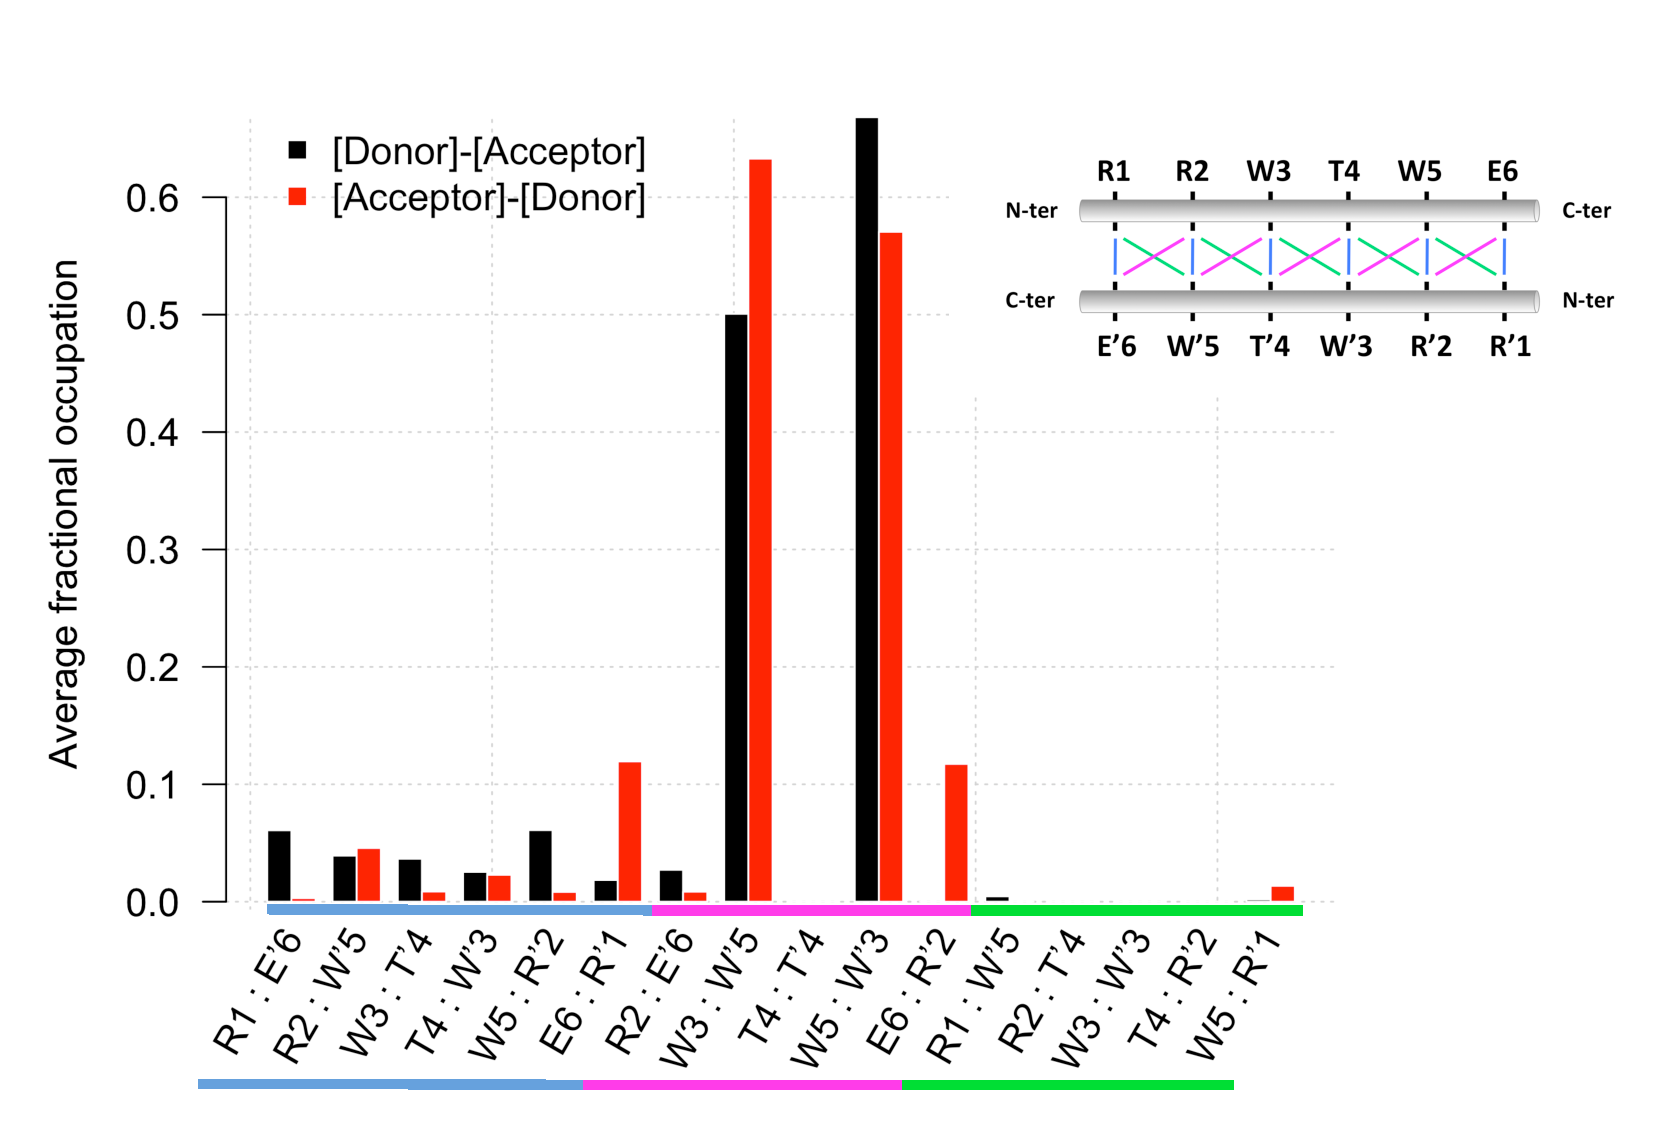
\includegraphics[width=0.7\linewidth]{3results_capsule/pics/merged_figures_beta_sheet} \label{fig:hb_beta_SIhere_hb}} \\
\bigskip
\subbottom[]{%
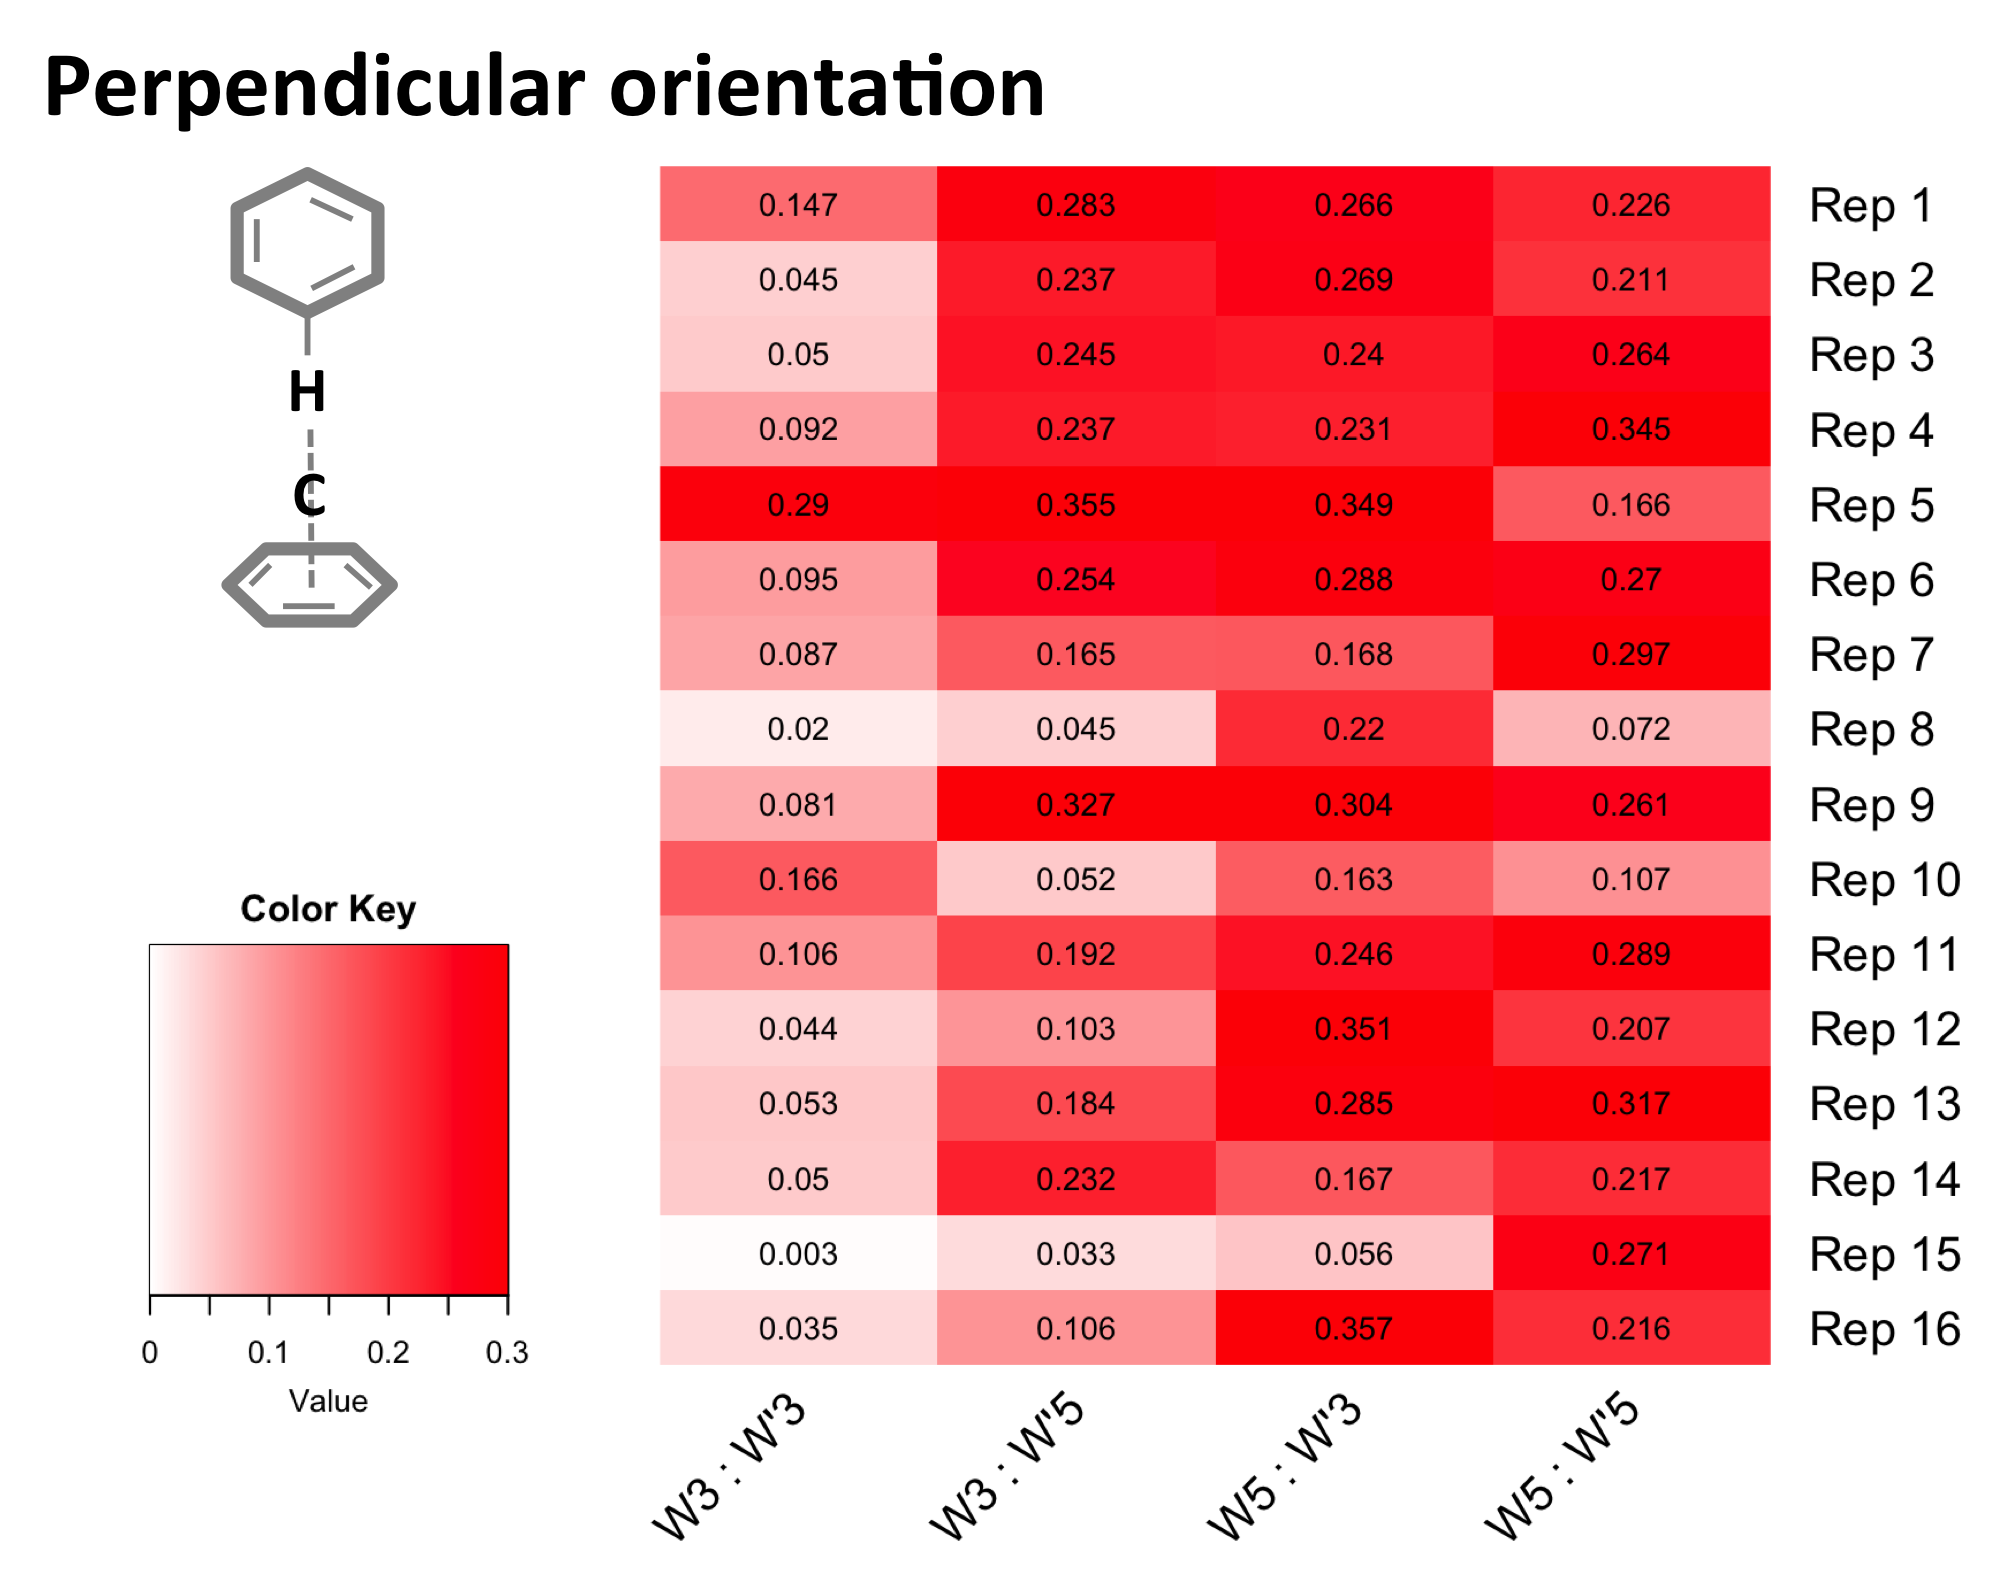
\includegraphics[width=0.47\linewidth]{3results_capsule/pics/pi_stacking_plot_part1} \label{fig:hb_beta_SIhere_pi1}} \hspace{0.2cm}
\subbottom[]{%
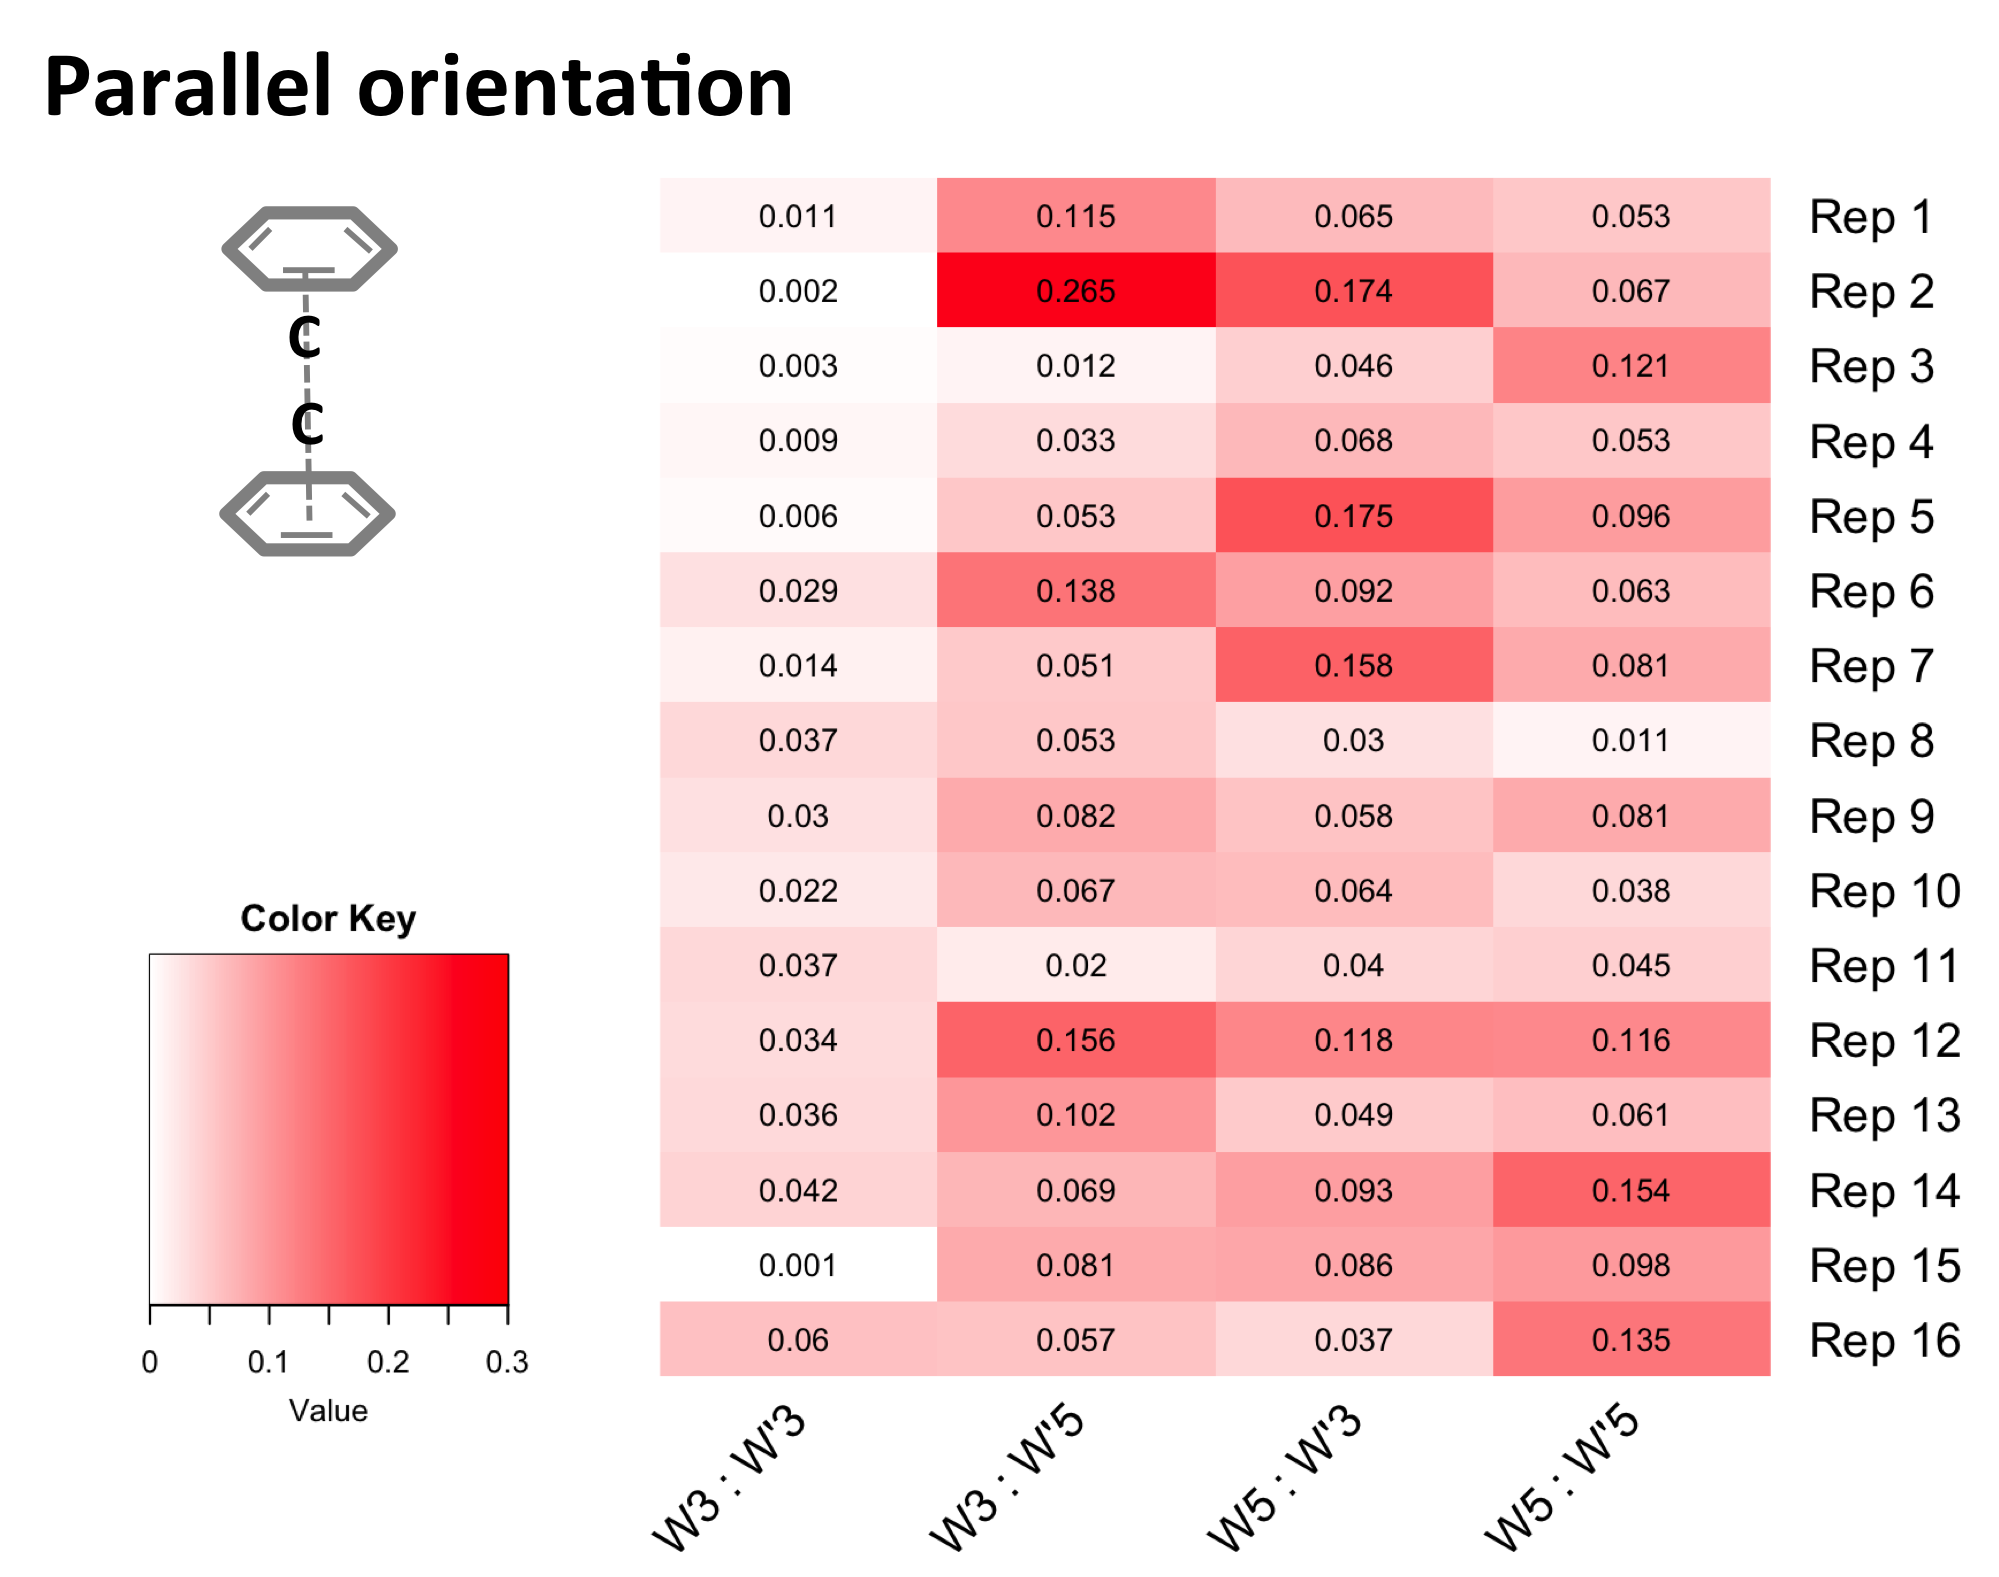
\includegraphics[width=0.47\linewidth]{3results_capsule/pics/pi_stacking_plot_part2} \label{fig:hb_beta_SIhere_pi2}}
\caption[Hydrogen bonds between RRWTWE $\beta$-sheet]{(a) Presence of backbone hydrogen bonds between amino acids in two facing antiparallel RRWTWE chains. The top right inset shows a scheme of the initial configuration. All the pairs highlighted in blue, green and pink are reported in the histogram; the same color code appears in the bar labels. Occupancy is averaged over 16 simulations of 20 ns. (b, c) For each replica and possible pair of facing Tryptophan residues in the $\beta$-sheet, the map gives the fraction of time for which a parallel or perpendicular $\pi$-stacking interaction has been observed. The second and fourth column correspond arrangement with the most populated hydrogen bonds.}
\label{fig:hb_beta_SIhere}
\end{figure}

\section{Modelling the assembly} \label{sec:build}

As previously mentioned, the antimicrobial sequence of capzip is designed with opposite charges at its extremes to favour an antiparallel $\beta$-sheets pairing with other copies of itself.
%
MD simulations of two RRWTWE sequences paired in this fashion confirm that the assembly is stabilised by opposite charge interactions (with statistics gather over 16 replicas, each run for 20 ns).
%
Moreover, backbone hydrogen bonds form between Tryptophan residues of facing strands, after a rearrangement of the mutual position of the backbones (Figure \ref{fig:hb_beta_SIhere_hb}).
%
Finally, $\pi$-stacking contributes to the interaction as well, albeit in minor measure (Figure \ref{fig:hb_beta_SIhere_pi1}, \subcaptionref{fig:hb_beta_SIhere_pi2}).
% SAY HOW WE COMPUTED IT
\begin{figure}[t]
\centering
\subbottom[]{%
    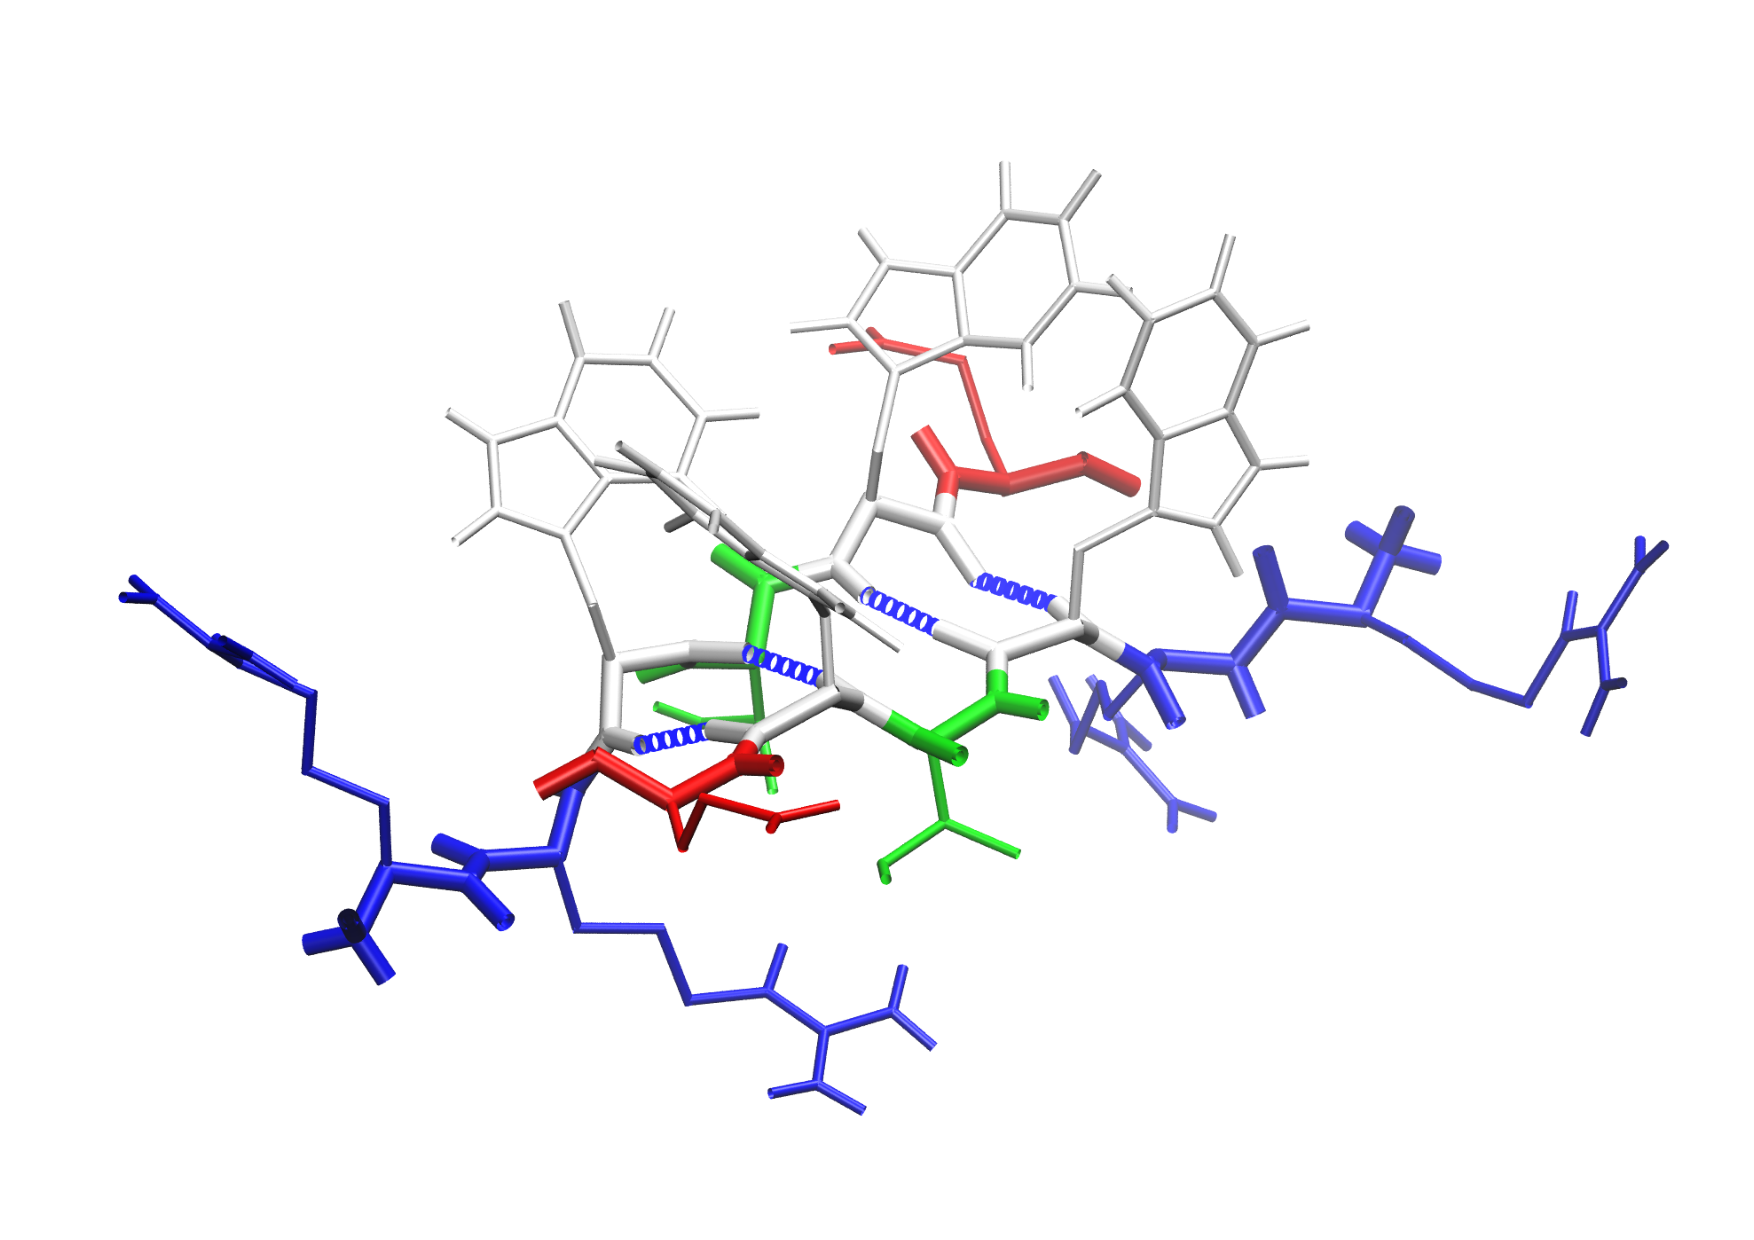
\includegraphics[width=0.4\linewidth]{3results_capsule/pics/beta_trpHbonds} \label{fig:BTI_vmd_1} }
\hspace{0.05\linewidth}
\subbottom[]{%
	\includegraphics[width=0.4\linewidth]{3results_capsule/pics/beta_surf} \label{fig:BTI_vmd_1a}}
\subbottom[]{%
	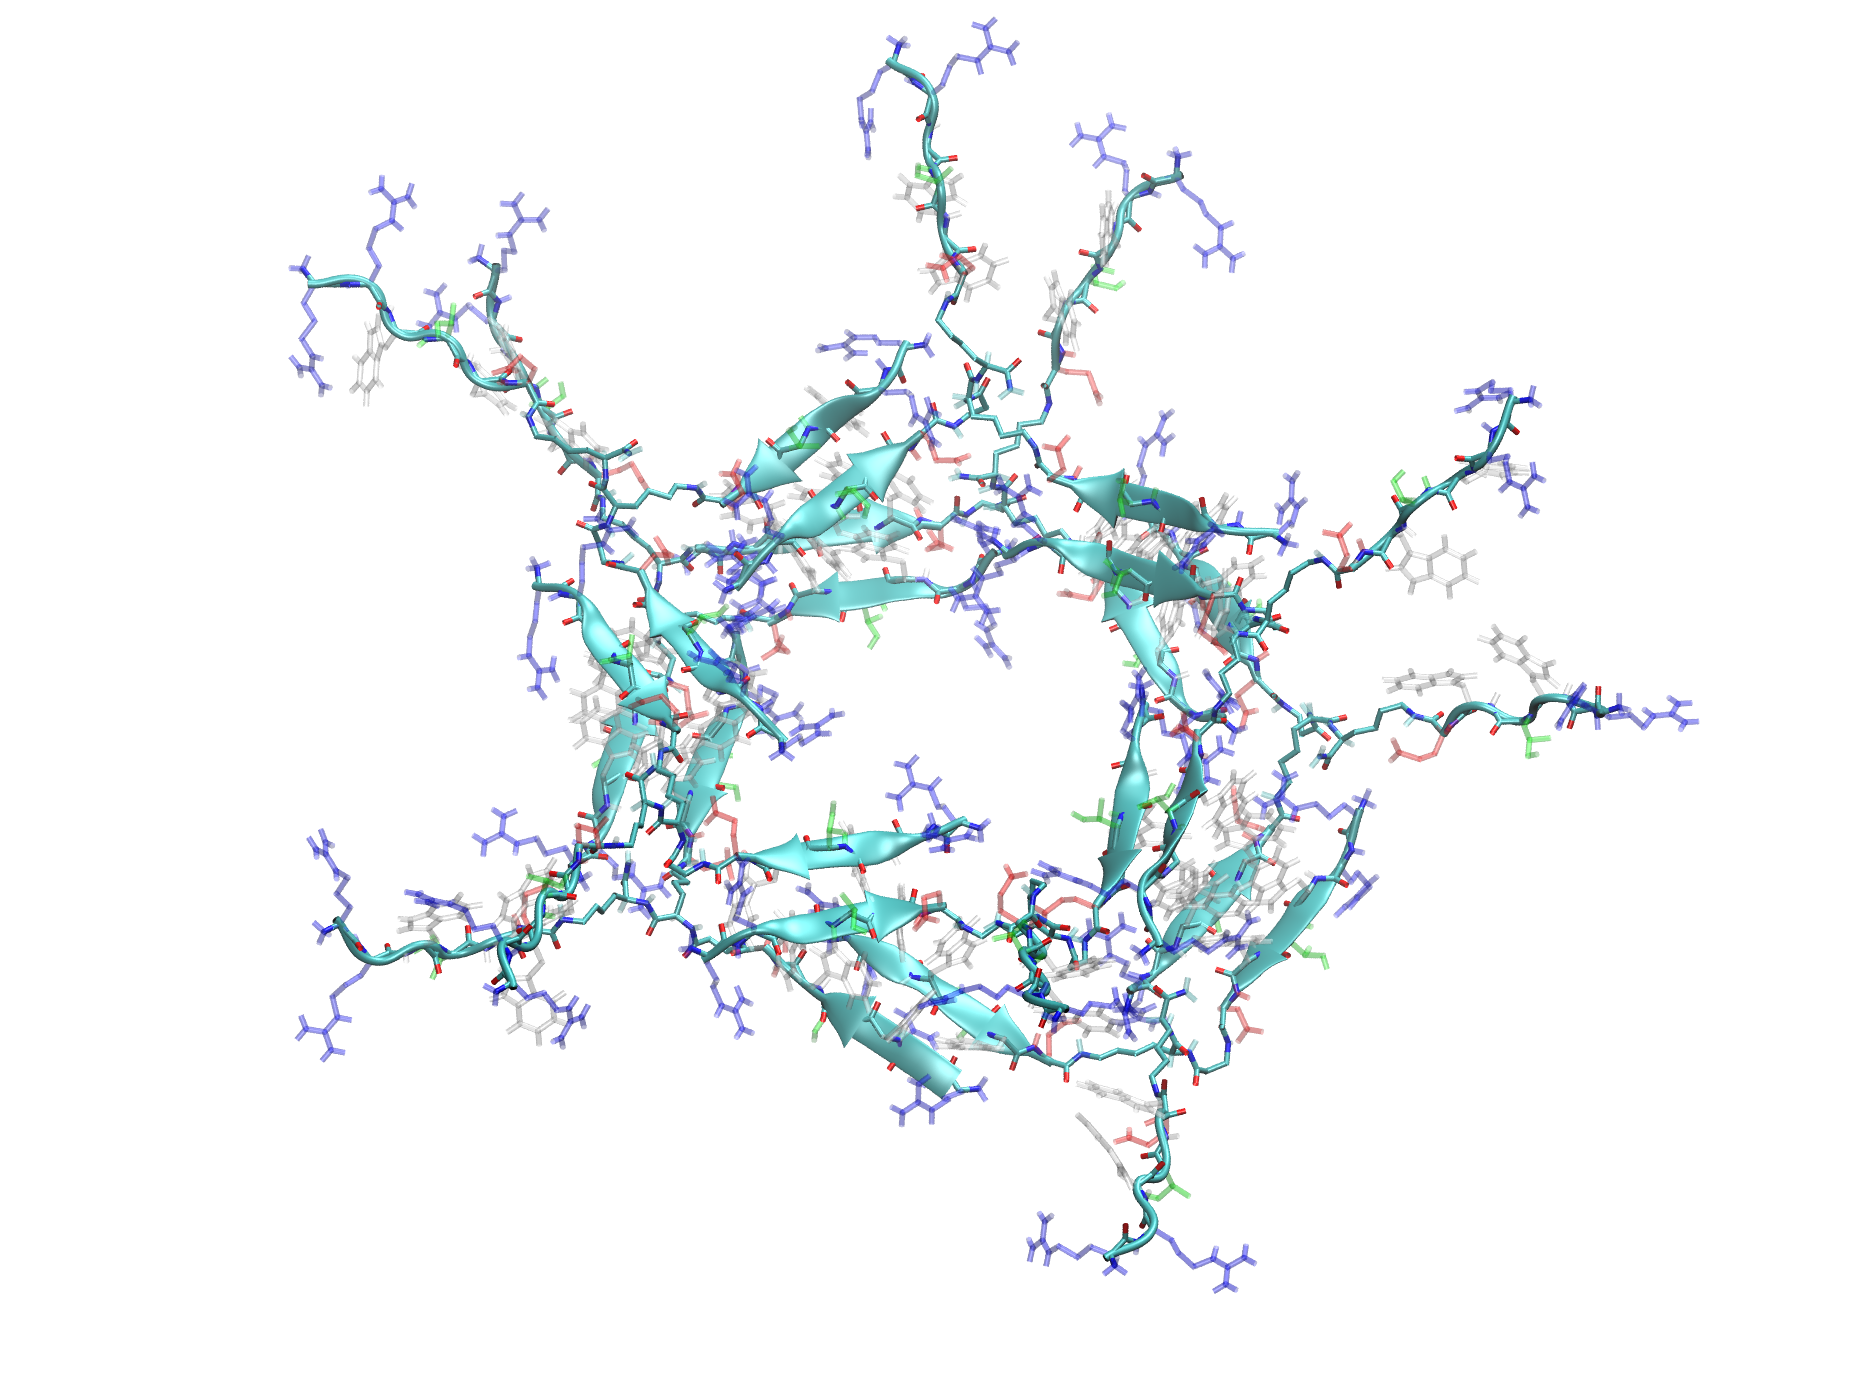
\includegraphics[width=0.45\linewidth]{3results_capsule/pics/pentamer_restype.png} \label{fig:BTI_vmd_2}}
\subbottom[]{%
	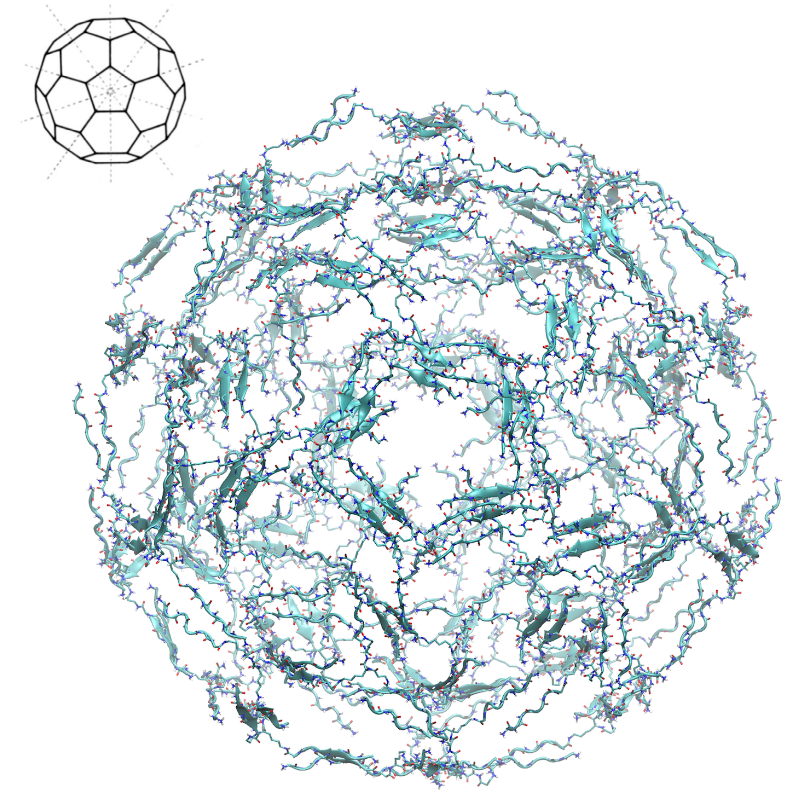
\includegraphics[width=0.45\linewidth]{3results_capsule/pics/soccer_empos_extern_superimposed.png} \label{fig:BTI_vmd_3}}
\caption[Building blocks of capzip assembly]{(a) Detail of $\beta$-sheet pairing with facing Tryptophan residues forming hydrogen bonds between their backbone atoms (bonds representation coloured by residue type, and hydrogen bond representation). (b) Two stacking $\beta$-sheets in surface representation, coloured by residue type. In white the partially buried hydrophobic patch. (c) A pentagonal subunit: ten antimicrobial molecules arranged in two stacking pentagons. Chains are paired in antiparallel $\beta$-sheets within each pentagon, and the two are interfacing with their Tryptophan residues in contact. (d) Atomistic structure of the buckyball simulated (bonds and cartoon representation) and geometrical model for comparison.}
\label{fig:BTI_vmd}
\end{figure}
%PUT YELLOW-GREEN SCHEME COLOUR AS IN THE FOLLOWING + SUPERIMPOSE TRANSPARENT SURFACE TO SHOW RESIDUE TYPE

The favourable hydrophobic interactions between Tryptophan residues result in the creation of a hydrophobic patch which includes four of them (in white in Figure \ref{fig:BTI_vmd_1} on one side of the $\beta$-sheet plane.
%
This creates an amphiphilic structure where the hydrophobic core is segregated from the remaining charged residues distributed at the other positions.
%
The combination of two stacking $\beta$-sheets, paired to match their hydrophobic patches, constitutes an effective supramolecular assemblies to reduce solvent exposure of such residues.

%\begin{figure}[h]
%\centering
%\begin{minipage}[b]{0.3\linewidth}
%\includegraphics[width=50mm]{pics/beta_bonds}
%\caption{}\label{fig:beta_vmd_1}
%\end{minipage}
%\begin{minipage}[b]{0.3\linewidth}
%\includegraphics[width=50mm]{pics/beta_half_surf}
%\caption{}\label{fig:beta_vmd_2}
%\end{minipage}
%\begin{minipage}[b]{0.3\linewidth}
%\includegraphics[width=50mm]{pics/beta_surf}
%\caption{}\label{fig:beta_vmd_3}
%\end{minipage}
%\caption{Two stacking antiparallel $\beta$-sheet formed by four copies of the RRWTWE sequence. a) Bonds and cartoon representations, coloured by atom; b) bottom sheet in surface representation, coloured by residue type; c) both sheets in surface representation, coloured by residue type. The exposed hydrophobic surface (white) is reduced with respect to an unpaired sheet (panel b).}
%\label{fig:beta_vmd}
%\end{figure}

This pairing strategy, however, needs to be applied in the context of full molecules assembly.
%
The quasi three-fold symmetry of capzip suggests a regular geometric arrangement.
%
The best examples of organised protein structures can be found in viral capsids, which are composed by the regular repetition of highly symmetric protein subunits.
%
Inspired by this, we tested whether a geometrical organisation can represent a stable capsule, choosing as representative geometry a truncated icosahedron (buckyball).

Preliminary atomistic simulations (100 ns) were run on a pentagonal subunit formed by ten molecules arranged in two stacking pentagons (as in Figure \ref{fig:BTI_vmd_2}), proving the cohesion between molecules belonging to the subunit. Specifically, the number of contacts between backbone $C_\alpha$s did not decrease in time but augmented slightly at the beginning, due to the compaction of the unpaired arms toward the core of the structure (Figure \ref{fig:penta_results_SIhere_1}). Moreover, for each pair of facing chains, it is computed the distance between their centres of mass. Figure \ref{fig:penta_results_SIhere_2} reports the variance of this distance over its average value, as a measure of the cohesion of the subunit, showing that in the majority of the cases less than 2\% of variability is observed.
% RUN SECOND SIMULATION?
\begin{figure}[t]
\centering
\subbottom[]{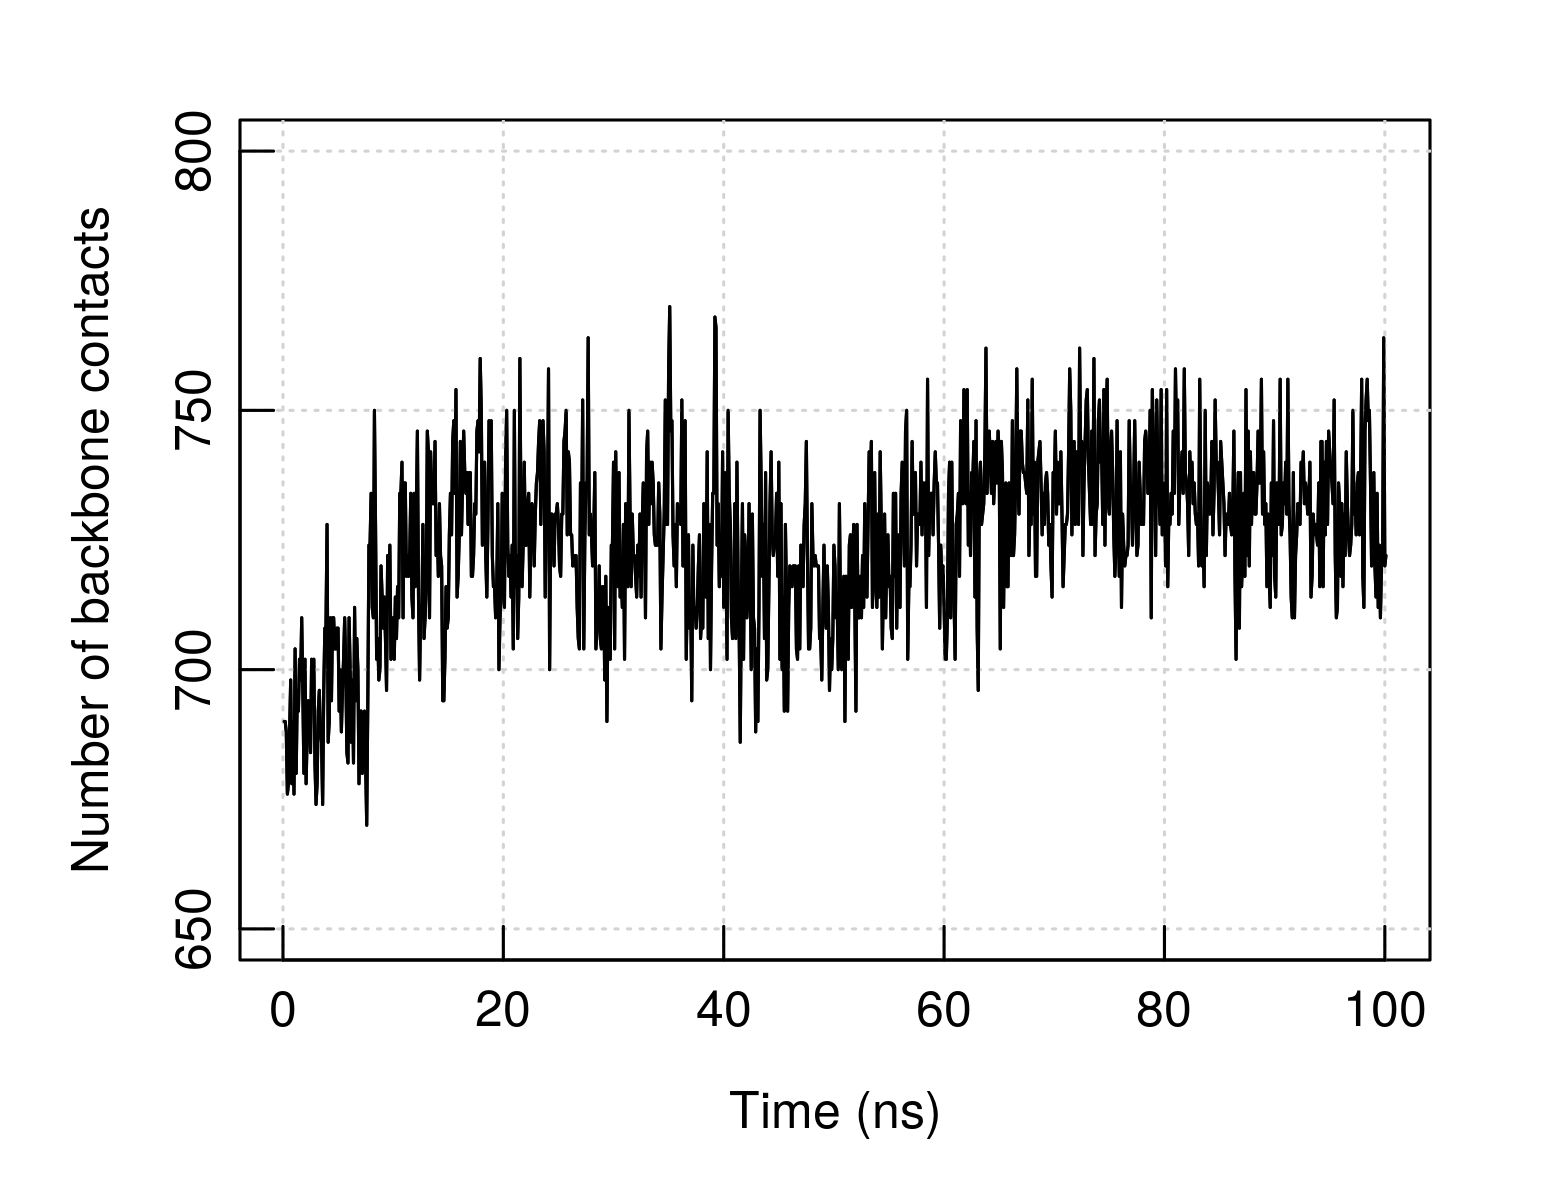
\includegraphics[width=0.45\linewidth]{3results_capsule/pics/bb_contacts.png} \label{fig:penta_results_SIhere_1}}
\subbottom[]{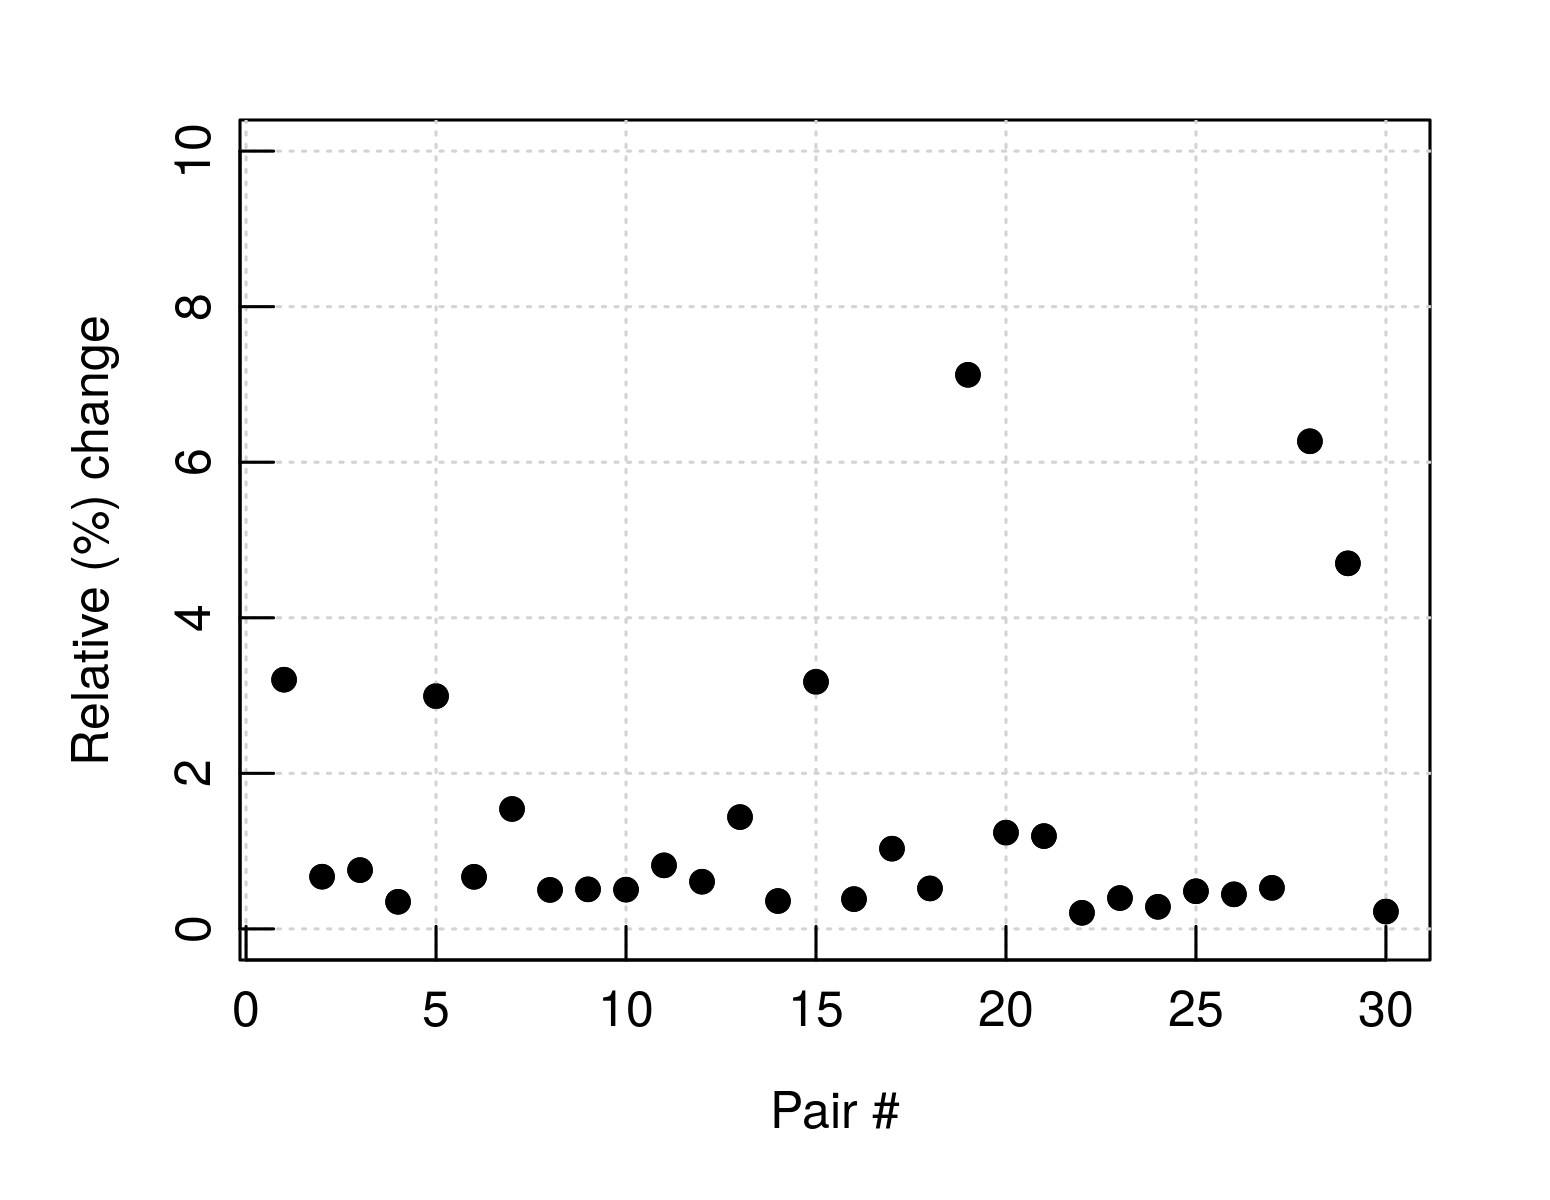
\includegraphics[width=0.45\linewidth]{3results_capsule/pics/chain_COM_distance.png} \label{fig:penta_results_SIhere_2}}
\caption[Cohesion measures on the pentagonal subunit]{(a) Number of backbone contacts during a simulation of a pentagonal subunit. (b) Variability of the inter chain average distance between facing chains. The 30 pairs defined as facing are the chains belonging to the same $\beta$-sheet (5 for each of the two stacking pentagons), and for each stacking $\beta$-sheet the 4 possible inter-pentagon (inter-layer) pairs of chains.}
\label{fig:penta_results_SIhere}
\end{figure}

The pentagonal subunit respects the building principles of a) $\beta$-sheet pairing between antimicrobial sequences and b) double layer structure to screen the hydrophobic patches, and will constitute a face of the icosahedron.
%
Each capzip molecule is centred in one vertex of the polygon, with the branches laying alongside the edges departing from it. On each edge two branches coming from opposite sides meet in an antiparallel fashion. When possible, a $\beta$-sheets with paired Tryptophan residues is organised (as in Figure \ref{fig:BTI_vmd_1}). The stacking pentagons interact through the hydrophobic patches of their $\beta$-sheet which are arranged in stacked positions.

The full truncated icosahedron was assembled from twelve pentagonal subunits (Figure \ref{fig:BTI_vmd_3}). As each subunit is formed by two stacked pentagons, the resulting structure has two concentric layers, for a total of 120 molecules, and initial radius of 7.7 nm.
%
This geometry represents a minimal model of the possible structures of capzip assembly in solution as, given the flexibility of the molecule, different geometries are possible, though proceeding from analogous interactions between the components.
%
The final structure was simulated at atomistic and coarse grain levels, respectively with the GROMOS 53a6 \cite{Oostenbrink2004}, SIRAH \cite{Machado2018} and MARTINI \cite{Marrink2007, Monticelli2008} force fields (with both standard and polar water \cite{Yesylevskyy2010} to compare the two models).
% LEAVE?
From the final configurations of the MARTINI coarse grain model (standard water), atomistic coordinates were obtained and simulated, to be compared with the original atomistic dynamics.
%
%Proving the stability at different timescales ascertains the characteristics that favour the assembly and identify the ones with suboptimal fitness to select them for improvement.
Moreover, additional simulations were run at all the coarse grain levels on a structure made of one layer only (i.e. build from pentagonal block make by one pentagon only), to prove whether the bilayer structure was more energetically favoured.

A multiscale analysis is needed also to investigate the antimicrobial activity. Being highly costing to simulate a full truncated icosahedron on a bilayer patch at the atomistic level, the pentagonal subunit employed to build the complete structure (Figure \ref{fig:BTI_vmd_2}) was taken as representative of the latter. It was simulated close to the membrane plane, parallel to it, to avoid spending time in sampling non bound conformations (Figure \ref{fig:pL6_vmd_1}). This, together with a tailored use of an applied electric field (see Section \ref{sec:details}), will speed up simulations considerable.

To observe the natural binding of the peptide to the membrane, the process of the full buckyball approaching a model membrane was simulated with a MARTINI coarse grain description (Figure \ref{fig:pL6_vmd_2}).

% TRUE ONLY IF COMPLETED DPPC
Two membrane patches were simulated for both resolutions, a model bacterial and a model mammal membrane, to identify the different interactions with the peptide. The first one presents 25\% of anionic lipids (DLPG), and the rest are zwitterionic (DLPC), while the second has only DLPC lipids.

\begin{figure}[t]
\centering
\subbottom[]{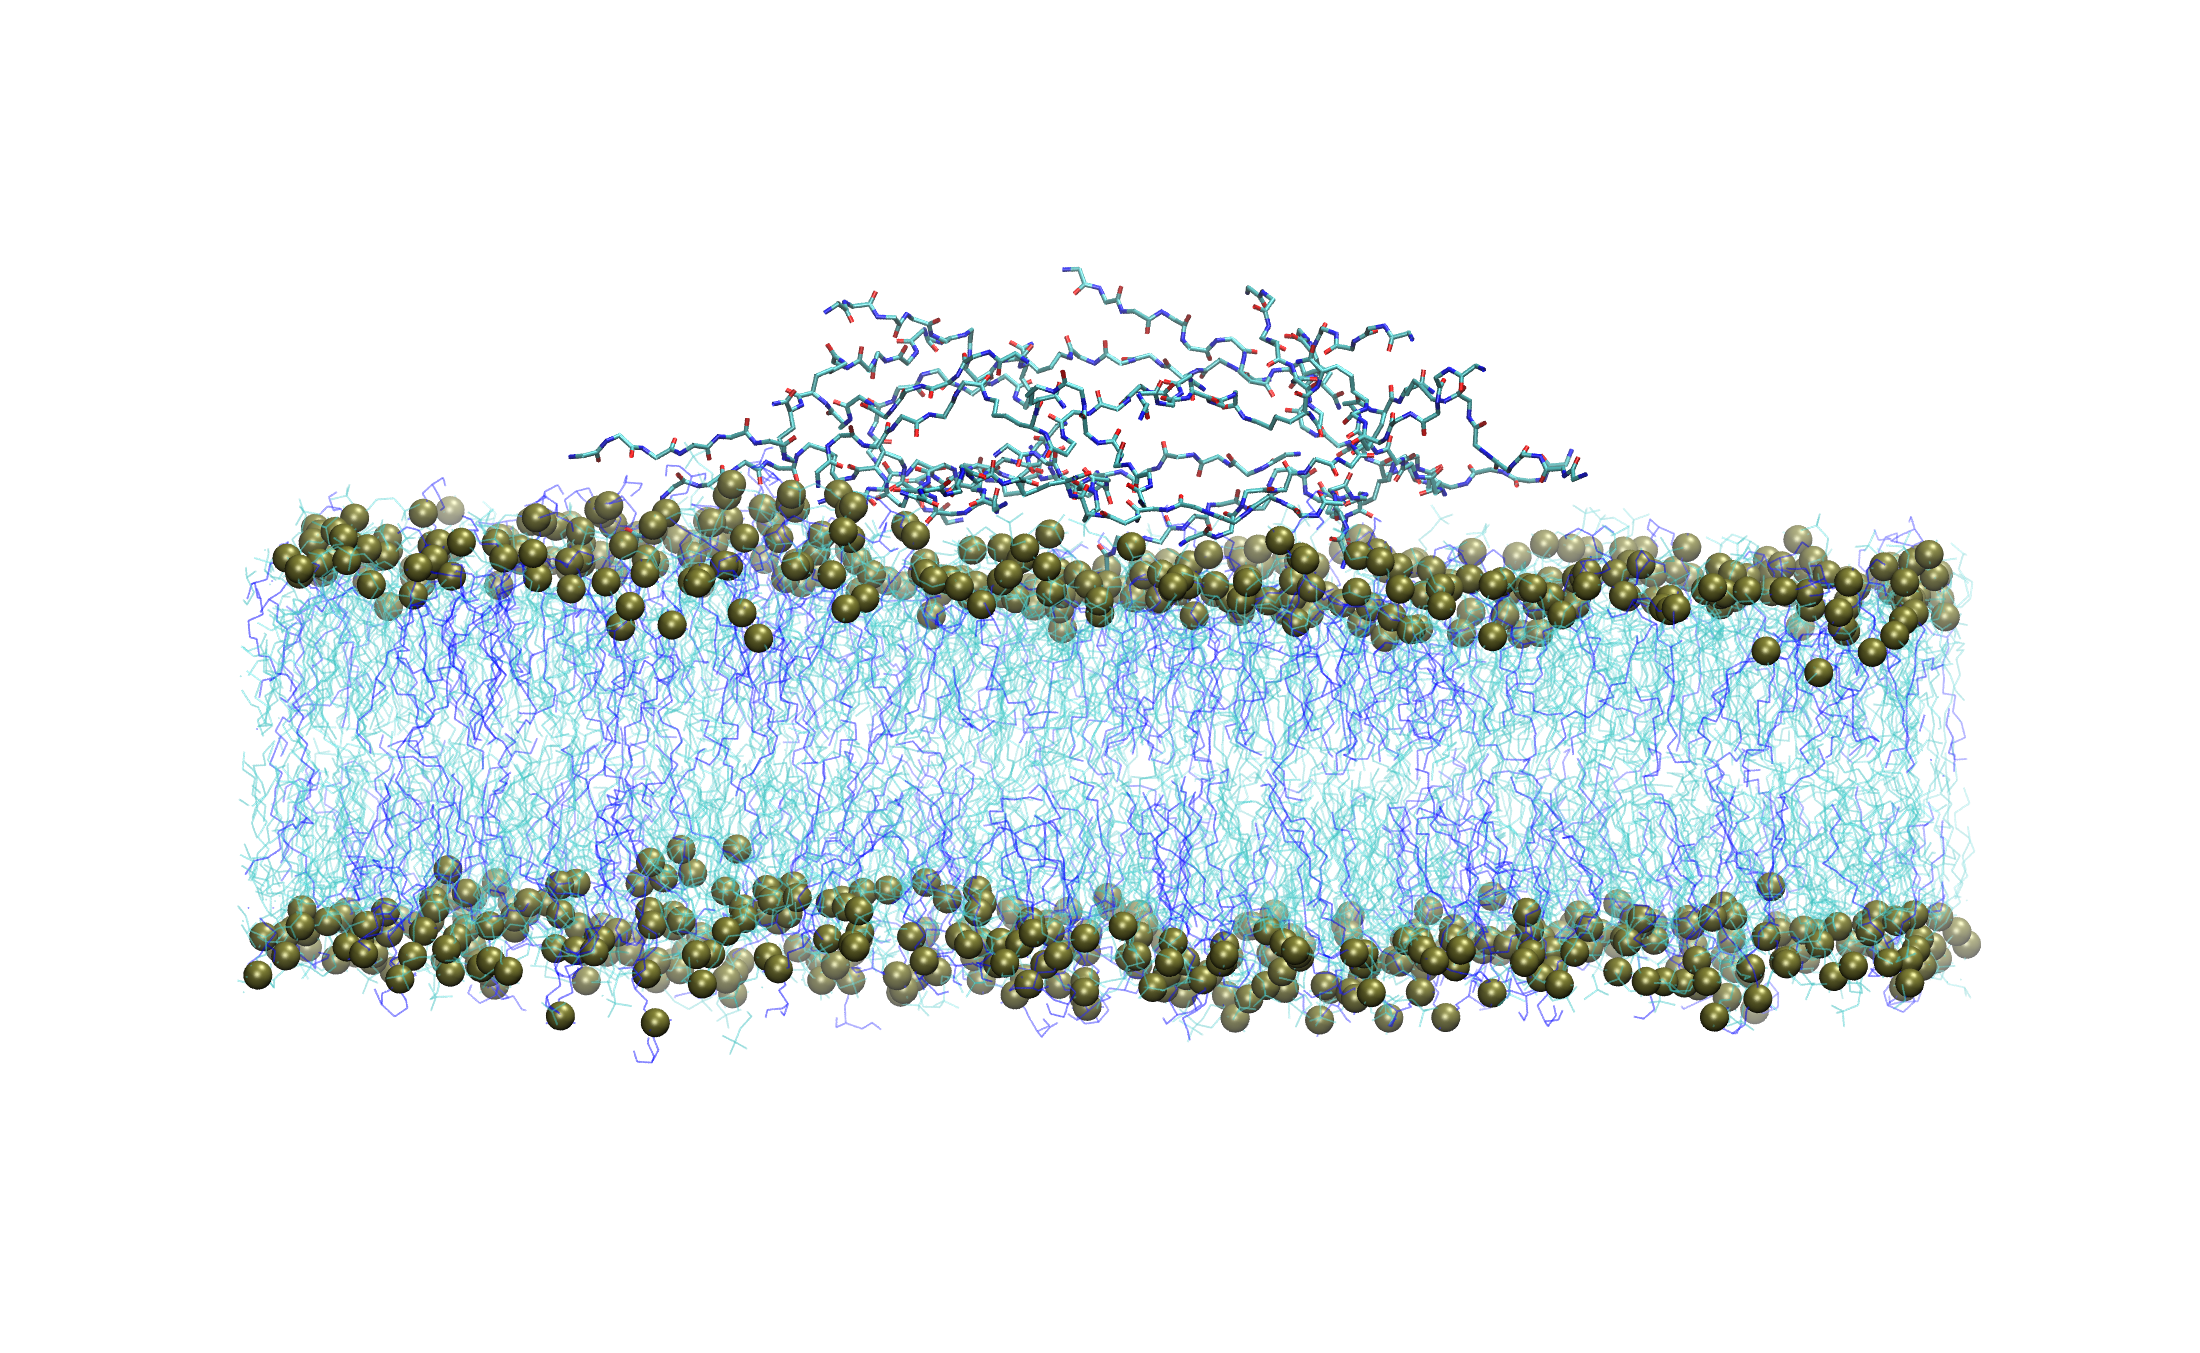
\includegraphics[width=0.45\linewidth]{3results_capsule/pics/pL6_Pramp_pic2.png} \label{fig:pL6_vmd_1}}
\subbottom[]{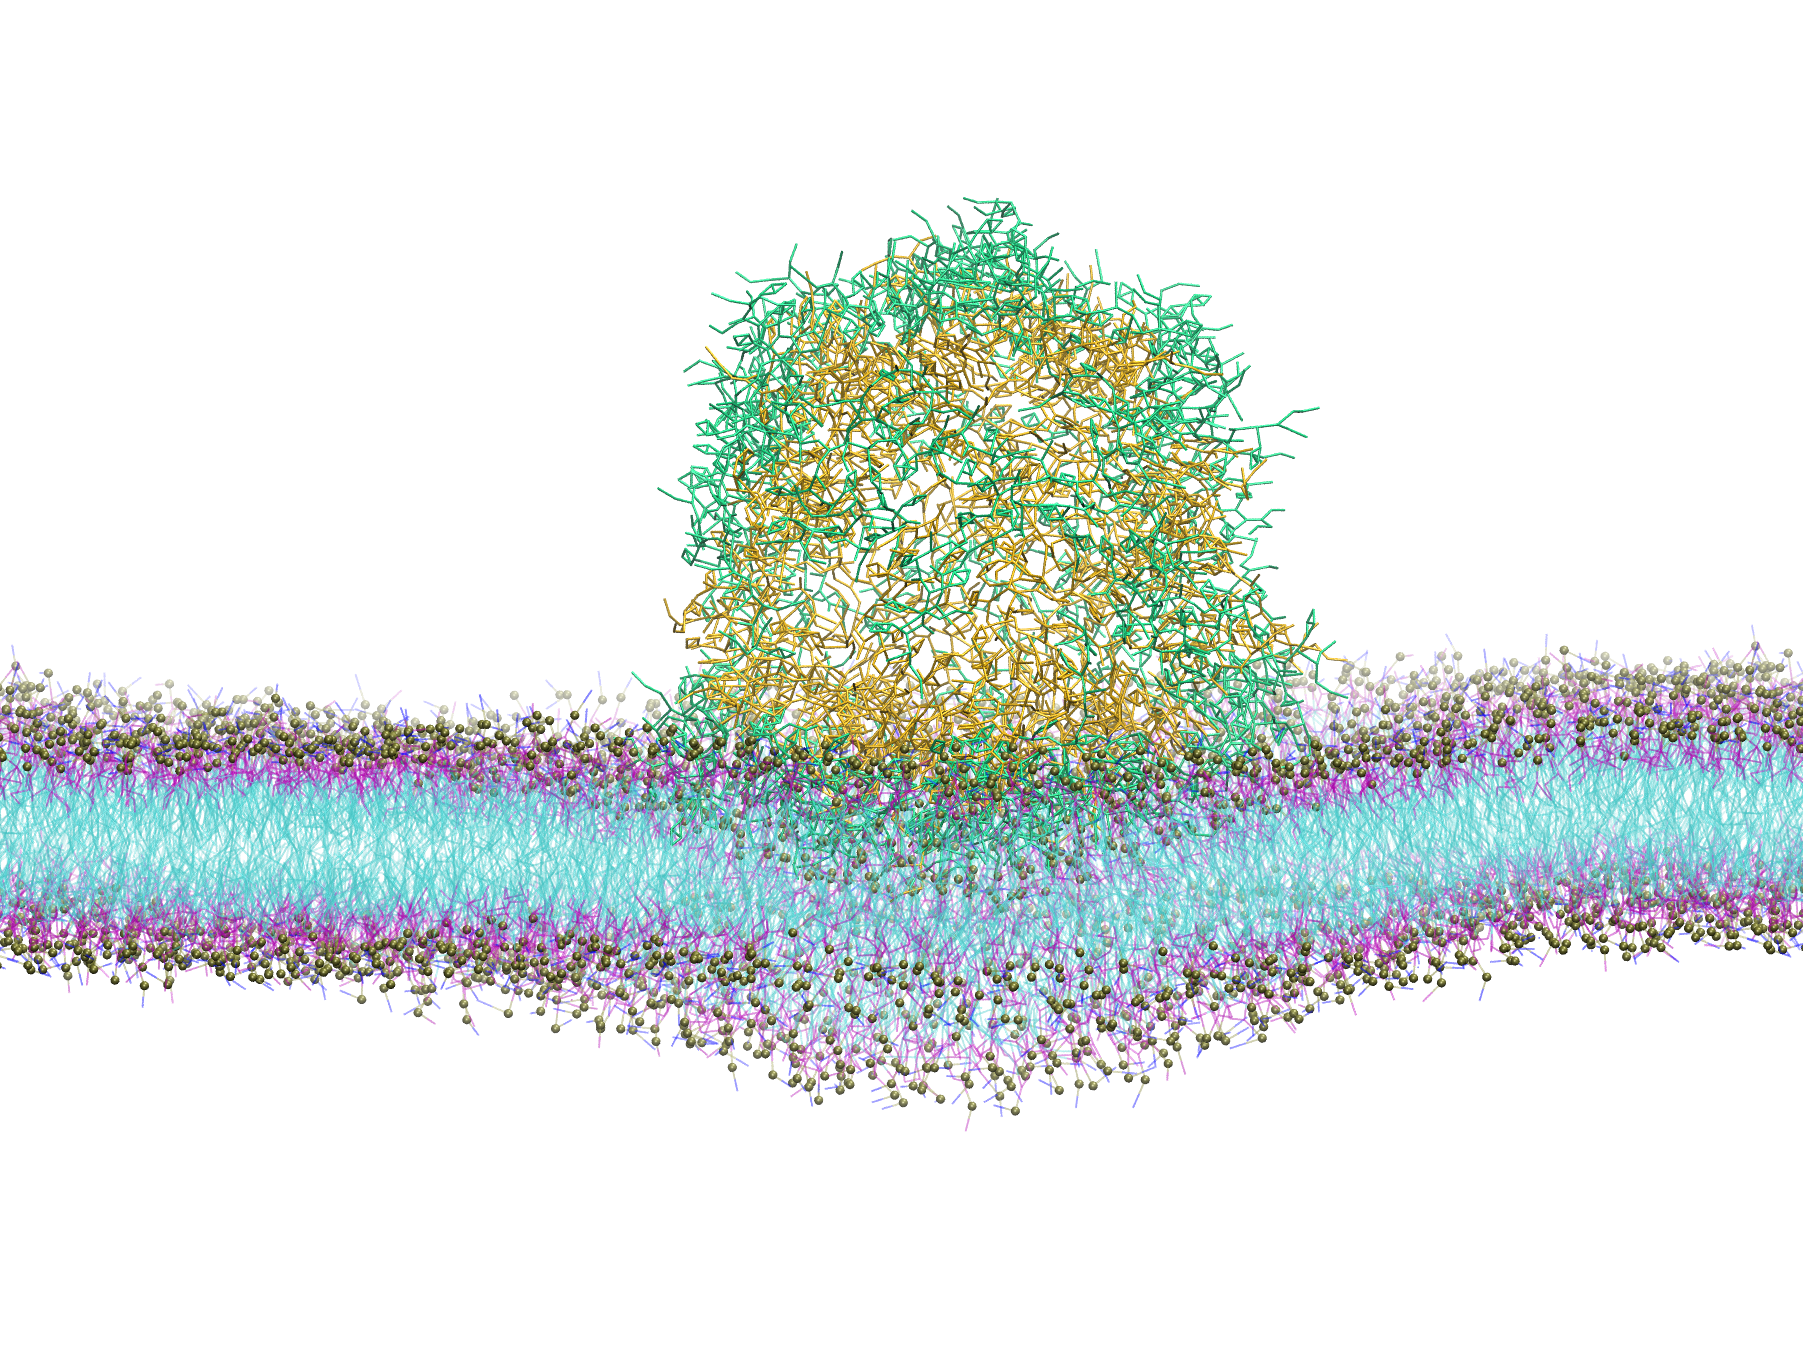
\includegraphics[width=0.45\linewidth]{3results_capsule/pics/fig7_irene.png} \label{fig:pL6_vmd_2}}
\caption[Snapshot of simulations of capzip on model membranes]{(a) Atomistic structure of a pentagonal subunit on a 740 lipid bacterial model membrane of composition DLPC:DLPG 3:1 (initial configuration). Peptide backbone in line and cartoon representation; lipid in cyan lines (DLPC) and blue ones (DLPC), all lipids phosphate in golden van der Waals beads. (b) Coarse grain (MARTINI) representation of the buckyball on a 2880 lipids bacterial model membrane (final configuration of the trajectory). Protein in bonds representation: green outer buckyball layer, yellow inner one. Lipid in line representation, coloured by bead type, and lipids phosphate in golden van der Waals beads.}
\label{fig:pL6_vmd}
\end{figure}


\section{Simulations details} \label{sec:details}

\paragraph{Atomistic simulations}
All simulations were performed with the GROMACS software, version 5.5 and 2016 \cite{Berendsen1995,Abraham2015,gromacs_man}. 

The atomistic coordinates for the peptidic supramolecular assemblies described in Section \ref{sec:build} were built combining GROMACS tools and the MOE software \cite{moe}.
%
Simulations were run with the GROMOS 53a6 force field \cite{Oostenbrink2004}. Parameters for the central residue connected with the peptidic chains are computed with the ATB software \cite{Malde2011, Koziara2014}; the ones for the joining bonds are derived from tabulated values of analogous peptide bonds. 

The systems were solvated with SPC water \cite{Berendsen1981} and counter ions were added (Na$^+$ or Cl$^-$); further ions are introduced to reach the concentration of 150 mM, to reproduce the experimental conditions.
%
For simulations of a single $\beta$-sheets and of the pentagonal subunit, the systems were energy minimised with a steepest descent algorithm, then equilibrated in the NVT ensemble with decreasing positional restraints at increasing temperatures (100 K, 200 K, 250 K, 300 K and respectively 1000, 1000, 500, 250 kJ/mol$\cdot$nm$^2$ restraints, 100 ps each); then in the NPT ensemble, without restraints, at the same temperatures steps and for the same time. Production was followed for 100 ns.

For the truncated icosahedron structure the above equilibration was still insufficient. Due to the construction procedure, two thirds of the branches are not properly paired along the edges.
%
Therefore, after an NVT equilibration as above, strong flat-bottom restrains (1000 kJ/mol$\cdot$nm$^2$) were placed between the center of mass of imperfectly aligned branches throughout the NPT heating, to penalise their mutual separation with respect to their initial distance (100 ps runs at 100 K, 200 K and 250 K and 35 ns at 300 K).
%
This was followed by a series of 10 ns runs at 300 K with decreasing restraints strength (750, 500 and 250 kJ/mol$\cdot$nm$^2$) and by a free production run (100 ns).
%
Three different replicas were run, generated from the final configuration of the 300 K NPT run with 1000 kJ/mol$\cdot$nm$^2$ restraints.

Throughout all the simulations, the temperature was maintained by independently coupling the protein and the solvent (plus ions) to two external temperature baths using a velocity rescale thermostat \cite{Bussi2007} with coupling constant $\tau _T$ of 0.1 ps. The pressure was kept at 1 bar by Berendsen \cite{Berendsen1984} or Parrinello-Rahman barostat \cite{Parrinello1981} (for the equilibration phases and the production run respectively) using an isotropic coupling, with isothermal compressibility 4.5 $\times$ 10$^{-5}$ bar$^{-1}$ and coupling constant $\tau_P$ of 1 ps. Electrostatic interactions were treated using the smooth Particle Mesh Ewald (PME) algorithm \cite{Essmann1995}, with a short-range cutoff of 0.9 nm. The van der Waals interactions were treated with a plain 0.9 nm cutoff. A SPC water model \cite{Berendsen1981} is used. All atomistic dynamic runs were performed using a 2 fs time step. An overview of simulations of peptide assembly in solution is given in Table \ref{table:sim_solution}.

\begin{figure}[t]
\centering
 \def\arraystretch{1.6}
\begin{tabular}{l|ccc}
 \multicolumn{4}{c}{\textbf{Capzip in solution simulations}} \\
 \hline
 System (Nr peptides) & Model & Time (ns) & Replicas \\
 \hline
 $\beta$-sheet (Fraction) & GR & 100 & 32 \\
 Pentagon-bilayer (10) & GR & 100 & 1 \\
 Buckyball bilayer (120) & GR & 100 & 3 \\
 Buckyball bilayer \& monolayer (120) & SI & 1000 & 3 \& 1 \\
 Buckyball bilayer \& monolayer (120) & MA & 1000 & 3 \& 2 \\
 Buckyball bilayer \& monolayer (120) & MA\_P & 1000 & 2 \& 1 \\
% \textbf{redo?} Backmapped buckyball (120) & GR & 100 & 3 \\
 \hline
 \end{tabular}
\captionof{table}{Table of simulations of capzip assembly in water. Model specifies the force field: GR = united atom GROMOS 53a6 \cite{Oostenbrink2004}, SI = coarse grain SIRAH \cite{Machado2018}, MA = coarse grain MARTINI \cite{Marrink2007, Monticelli2008}, MA\_P = coarse grain MARTINI with polar water \cite{Yesylevskyy2010}.}
\label{table:sim_solution}
\end{figure}

The atomistic coordinates for the bacterial model membrane patch were built with the PACKMOL software \cite{Martinez2009}, from pdb files of a single DLPC \cite{PogerOrig} and DLPG \cite{Kukol2009} molecule. Two patches were built, made respectively of 512 and 740 lipids, with composition DLPC:DLPG (3:1). The initial area per lipid was set to 7 nm$^2$, above the values found experimentally for either lipid species (0.608$\,\pm\,$0.012 nm$^2$ for DLPC \cite{Kucerka2011} and 0.656$\,\pm\,$0.012 nm$^2$ for DLPG \cite{Pan2012}). The correct area per lipid of the mixture was reached during a 400 ns equilibration, the final configuration of which was used for simulations with the peptide on the membrane.
% VERIFY WE CAN RUN IT!!!
A similar procedure was held for DLPC, producing a patch of 748 lipids with an initial area per lipid of 0.656$\,\pm\,$0.012 nm$^2$. This patch was used for control simulations against the 740 lipids bacterial one.

The initial configuration of atomistic simulations of the peptide on the membrane was generated from the equilibrated lipid bilayer (after 400 ns run) and the equilibrated pentagonal subunit (after 100 ns run with positional restraints on the C$_\alpha$), placing the pentagon plane parallel to the membrane one and close to it (Figure \ref{fig:pL6_vmd}).
%
The inflategro \cite{Kandt2007} script was used to solve the partial overlap of the peptide side chains with the lipid molecules, removing the ones overlapping.
%In the configuration chosen, 6 and 3 lipids are removed from the 512 and 740 lipids bacteria membrane patch respectively and 13 from the 748 mammalian membrane one.
%
The sizes of the two patches fit the pentagonal subunit with respectively 3.5 nm and 5.4 nm distance between its periodic boundary images (along both $x$ and $y$).

For simulations involving membranes, the version 54a8 \cite{Oostenbrink2005, Reif2013} of the GROMOS force field was employed. Lipid parameters were taken from \cite{PogerOrig} for DLPC, while for DLPG they were built from the ones available in the literature for POPG \cite{Kukol2009}.

The simulations set-up parameters are as above, except for the use of three thermal coupling groups (peptide, membrane, water plus ions), a semi-isotropic pressure coupling, and a larger cut off radius for both Coulomb and van der Waals interactions (1.2 nm). Additionally, for the 512 lipids membrane, a Reaction Field \cite{Tironi1995} was used instead of PME long range electrostatic treatment. Control simulations on membrane patches without peptide showed that the results in terms of area per lipid are compatible with the ones obtained from PME.

Each membrane patch was first equilibrated for 50 ps in NPT conditions at 50 K, then the temperature was gradually increased up to 300 K in 500 ps, and finally a 400 ns production was run. The final configuration was used as initial structure for the peptide-membrane simulations. A similar equilibration procedure was followed for peptide-membrane systems.

Additional simulations were performed applying an external electric field to the membrane, from the side hosting the peptide to the opposite one, to mimic the membrane potential and verify how the presence of the peptide affects the membrane response to external stimuli.
%
In a first test performed on the 512 lipids bacterial patch, the field was increased by 20 mV/nm steps every 200 ns, until reaching the electroporation value, which resulted to be 130 mV/nm.
%
For the bacterial membrane patches of both sizes, other simulations were performed starting from the unperturbed membrane configuration and the threshold field, in three replicates each. Three control runs were performed on the 512 patch without peptide, at the threshold value of the field, and one at the higher value of 140 mV/nm.

To be noticed that membrane field is estimated around 20 mV/nm across mammalian membranes and 35 mV/nm (from, respectively, a -70/-90 mV and -130/-150 mV potential \cite{Wilson2011} and an estimate membrane thickness of 4 nm), but previous computational work explored the effects of fields up to 500 mV/nm \cite{Tieleman2004, Bockmann2008, Piggot2011}, to witness poration within the simulations time, according to the resources available at the time.

An overview of simulations of peptide-membrane systems is given in Table \ref{table:sim_membr} (control simulations on pure membrane are listed in Table \ref{table:SI_sim_E}).

\begin{figure}[t]
\centering
 \def\arraystretch{1.6}
\begin{tabular}{ll|ccc}
\multicolumn{5}{c}{\textbf{Capzip on membrane simulations}} \\
\hline
 & System &  Model & Time (ns) & Replicas\\
 \hline
 \multirow{4}{*}{\rotatebox{90}{Bacterial}} & 10 peptides, 512 lipids & GR & 500 & 2 \\
 & 10 peptides, 740 lipids & GR & 500 & 1 \\
 & Buckyball, 2880 lipids & MA & 10000 & 2 \\
 & Buckyball, 2880 lipids & MA\_P & 10000 & 1 \\
 \hline
 \multirow{3}{*}{\rotatebox{90}{Mammalian}} & 10 peptides, 740 lipids & GR & 500 & 1 \\
 & Buckyball, 2880 lipids & MA & 10000 & 1 \\
 & Buckyball, 2880 lipids & MA\_P & 10000 & 1 \\
 \end{tabular}
 \begin{tabular}{ll|cccc}
 \hline
 \multicolumn{6}{c}{\textbf{Electroporation simulations}} \\
  \hline
  & System & Model & Time (ns) & Replicas & E (mV/nm) \\
 \hline
 \multirow{2}{*}{\rotatebox{90}{Bact.}} & 10 peptides, 512 lipids & GR & 75, 20, 71 & 3 & -130 \\
 & 10 peptides, 740 lipids & GR & 60, 50, 70 & 3 & -130 \\
 \hline
 \multirow{2}{*}{\rotatebox{90}{Bact.}} & Buckyball, 2880 lipids & MA\_P & ?? & 1 & ??\\
 & Buckyball, 2880 lipids & MA\_P & ?? & 1 & ??s\\
 \hline
\end{tabular}
\captionof{table}{Table of simulations of peptide-membrane complexes. All the mentioned ones run at 150 mM concentration of NaCl. Models: GR = united atom GROMOS, MA = coarse grain MARTINI, MA\_P = coarse grain MARTINI with polar water. For electroporation simulations, the time refer to the rupture of the membrane. For electroporation simulations on pure membranes, see SI Table \ref{table:SI_sim_E}.}
\label{table:sim_membr}
\end{figure}

\paragraph{SIRAH coarse grain simulations}
SIRAH coarse grain simulations were run with the SIRAH force field \cite{Machado2018}. Peptide coordinates for the buckyball geometry were obtained from the atomistic ones using the converter distributed with force field. Parameters for the central residue were built from comparison with similar chemical moieties.

While for simulations of peptide assembly in solution we resorted to a multiscale procedure, comparing up to four force fields, for simulations on membrane we focussed only on atomistic and MARTINI simulations only. This has been performed in the interest of time, and following some concerns arisen in preliminary SIRAH runs of the capsule on a membrane, which showed an unstable behaviour (contraction and expansion of the membrane).
%
Given that there are little benchmarks so far on the performances of SIRAH for lipids, and none for systems as large as the one studied here, we are continuing pursuing the investigation at an exploratory level, working in contact with the developers of the force field to help elucidating its limitations and work out the best equilibration procedure to treat large membrane patches.

For SIRAH simulations, the temperature coupling was performed with a velocity rescale thermostat \cite{Bussi2007} and coupling constant $\tau _T$ of 0.1 ps, and the pressure coupling at 1 bar pressure, with 4.5 $\times$ 10$^{-5}$ bar$^{-1}$ isothermal compressibility, using a Parrinello-Rahman barostat \cite{Parrinello1981} with a $\tau _P$ of 6 ps. Electrostatic interactions were treated using the PME algorithm \cite{Essmann1995}, with a short-range cutoff of 1.2 nm and relative dielectric constant of 1. The van der Waals interactions are treated with a plain 1.2 nm cutoff.

After energy minimization, a 4 ns NVT equilibration was run at 300 K, followed by a 10 ns NPT run, both with positional restraints (1000 kJ/mol$\cdot$nm$^2$) on the solute. Two 10 ns run (NPT ensemble, 300 K) were then performed with backbone restraints of 1000 and 100 kJ/mol$\cdot$nm$^2$, respectively. Similar to the procedure adopted for the atomistic simulations, during the latter, flat bottom positional restraints (1000 kJ/mol$\cdot$nm$^2$) were enforced on the unpaired branches during the NPT. Three additional 10 ns equilibrations were run at 300 K, with no backbone restraints and decreasing flat bottom ones (respectively 750, 500 and 250 kJ/mol$\cdot$nm$^2$). Finally the production run was carried on for 1 $\mu$s. All runs were performed with a 20 fs time step.

\paragraph{MARTINI coarse grain simulations}
For MARTINI \cite{Marrink2007, Monticelli2008} coarse grain simulations, peptide coordinates and parameters were obtained from the atomistic ones using martinize.py \cite{DeJong2013}, and pycgtool.py \cite{Graham2017} for the central residue. Parameters for the joining bonds were derived from tabulated values of analogous ones.

The bacterial and mammalian model membranes, hosting 2880 lipids each, were built with insane.py \cite{Wassenaar2015}, with composition DLPC:DLPG 3:1 and pure DLPC respectively. The simulations parameters used for lipids are consistent with Ref. \cite{SiewertJ.Marrink2003}. The peptide-membrane systems were built placing the buckyball at a minimum distance of 1 nm from the membrane surface.

For simulations performed with the standard water model, the temperature coupling was performed with a velocity rescale thermostat \cite{Bussi2007} with a coupling constant $\tau _T$ of 1 ps. An isotropic or semi-isotropic pressure coupling was applied (for peptide in solution or peptide on membrane simulations) at 1 bar pressure, with 4.6 $\times$ 10$^{-5}$ bar$^{-1}$ isothermal compressibility, using a Berendsen \cite{Berendsen1984} or Parrinello-Rahman barostat \cite{Parrinello1981} (equilibration and production phase respectively) with a $\tau _P$ of 12 ps. An isotropic or semi-isotropic coupling has been used for simulation without and with membranes respectively.
%
Coulomb interactions were treated with a Reaction Field scheme \cite{Tironi1995} and cut off radius of 1.1 nm, van der Waals interaction with a cut off scheme and the same cut off radius. The relative dielectric constant is set to 15.
%
Simulations performed with the polar water model were run with the parameters above, except the relative dielectric constant set to 2.5, and the choice of a PME scheme for the long range Coulomb interaction (1.2 nm cut off radius).

For simulations of the capsule in solution, for both water models, after energy minimization four 10 ns equilibration runs (NPT ensemble, 300 K, 10 fs time step) were performed with flat bottom positional restraints on the unpaired branches (respectively at 750, 500 and 250 kJ/mol$\cdot$nm$^2$) - as done for the other force fields.
%
Finally the production run was carried on for 1 $\mu$s. All runs were performed with a 20 fs time step.

It is interesting to notice that the MARTINI force field with the standard water model produce very similar results even without such refined equilibration procedure. However, we choose to follow it to have results more consistent with the other parametrisations and be certain that the differences observed are due only to the force field an not the equilibration procedure.

The membranes used in the simulations are equilibrated for 1 $\mu$s and the final configuration used to build the peptide-membrane system, together with the equilibrated capsule structure (before production). The full system is then after energy minimised and equilibrated for 500 ps.
%
Production is followed for 10 $\mu$s for simulations with the standard water, and 1 $\mu$s with polar water.

The adoption of the polar water model allows to perform electroporation experiments also with the MARTINI force field (while the standard water, not bearing a dipole, is unable to screen the externally applied electric field, resulting in unphysical effects).
%
We thus resorted to a procedure similar to the one employed for atomistic simulations, testing an external electric field of magnitde 20 mV/nm and 40 mV/nm, finding that the latter is sufficient to trigger electroporation in model bacterial membranes in less than 500 ns (while the former is not). It is likely that longer simulations would allow to observe this behaviour even with lower values of the force field, however, in the interest of time, we selected this value for further investigation.

Specifically, we selected a configuration from the early stages of poration (where the pore showed a diameter of 2 nm) and continue the simulations switching to an isotropic pressure coupling. Indeed, 


% MENTION???
%From the final configurations of MARTINI simulations of the buckyball in solution (standard water model), atomistic coordinates are obtained using the MARTINI backward tool (version 5) \cite{Wassenaar2014} and run for additional 200 ns with set up for atomistic simulations, to compare the original dynamic to one at a later time (as obtained with coarse grain simulations). This procedure is performed for two out of the three MARTINI-standard water replicas available.


\section{Analysis}

\paragraph{Simulations in solution}
Several structural analysis were performed on the outcome of the simulations of the buckyball in solution. Standard measures like the Radius of gyration ($R_g$), the Root Mean Square Deviation with respect to the initial configuration (RMSD) were computed (with GROMACS).
%
To get the average distribution of the mass of the capsule, the Radial Distribution Function (RDF) of the protein masses around their center of mass was computed (with GROMACS). The profile could be fitted with a Gaussian function (with the R \cite{??} software) as they presented negligible skewness, so that the position of its maximum can be taken as an average radius of the capsule, and its Full Width at Half Maximum (FWHM) as an estimate of the thickness of the bilayer.

The dynamical character of the structure was assessed computing the correlation of motion between the molecules. The central atom (or bead) from which the branches depart was taken as reference. For all the pairs $i$ and $j$ of such reference positions, the covariance of motion $\sigma^2(i,j)$ was computed (with GROMACS), where the covariance is the sum of the components along each axis: $\sigma^2(i,j) = \sigma^2(i,j)_x + \sigma^2(i,j)_y + \sigma^2(i,j)_z$. Then for each pair, this measure was normalised as:
\begin{equation}
corr(i,j) = \frac{\sigma^2(i,j)}{\sqrt{\sigma^2(i,i)\,\cdot\,\sigma^2(j,j)}}.
\end{equation}

Another structural measure concerns the pairing of the branches. Two branches are defined as paired if their center of mass is closer than a cut off distance of 1.2 nm. This simple measure discards any more precise information on the orientation of the chains with respect to each other, and aims at checking whether the network of molecules present in an ideal buckyball structure is maintained. In the ideal buckyball, contacts within the same layer sum up to 90 for each layer (for a total of 180 in a bilayer). This measure can be easily applied to any description (atomistic or coarse grain) without disagreement in the interpretation. The computational pipeline combines GROMACS tools and a post-processing in R language.

To characterise the chemical determinants that promote the assembly, we investigate the interactions between amino acids of different types, computing the number of contacts between backbone and side chains of single amino acids, filtered for the ones present a least 50\% of the simulation time, and classified them by amino acid type.
%
We define contacts between amino acids backbones if the C$\alpha$ of two residues (or the corresponding coarse grain bead) are closer than a cutoff distance of 0.6 nm; and between side chains if selected reference atoms in the side chain are closer than the same cut off; finally mixed ones if the proximity is between a C$\alpha$ and the side chain reference atom. As side chains reference, we took the heavy atom or bead farthest away from the backbone (respectively for GROMOS, SIRAH and MARTINI: CZ/SC2/BCZ for Arg, CZ2/SC4/BNE for Trp, OG1/SC1/BPG for Thr and CD/SC1/BCD for Glu). The functions to perform the analysis were built on the ones implemented in the MDAnalysis software (see Appendix --).

Further investigation has been carried on for atomistic simulations computing the hydrogen bonds between amino acids and grouping them by amino acid type and by region of occurrence (e.g. between two backbones, side chains or connecting a backbone atom and a side chain one).

Finally, the Solvent Accessible Surface Area was computed for each amino acid (with GROMACS). Its value was averaged in time and over all the residues of the same type. It was normalised over its reference value for each residue type X, obtained as the measure of the SASA of X from a Gly-X-Gly tripeptide. The resulting measure (named Q$_{SASA}$) takes into account the size of the side chain of each amino acid, giving a measure of exposure which can be compared between different residues. 
%
This normalisation is somewhat inappropriate for coarse grain models, however we employed it as it provides nevertheless a coarse regularisation for size effects.

\paragraph{Simulations on a membrane}


\section{Results: capsule in solution} \label{sec:results_cap}
% prima parla di atomistiche e tutto quello che c'e da dire. poi comincia confronto con cg. e parla di come si confermano cose oppure no. poi che con cg puoi confrontare con monomero
We list here the results for the capsule in solution first: starting from the atomistic simulations, we then proceed to compare the outcome with the ones obtained by different coarse grain models.

\begin{figure}[t]
\centering
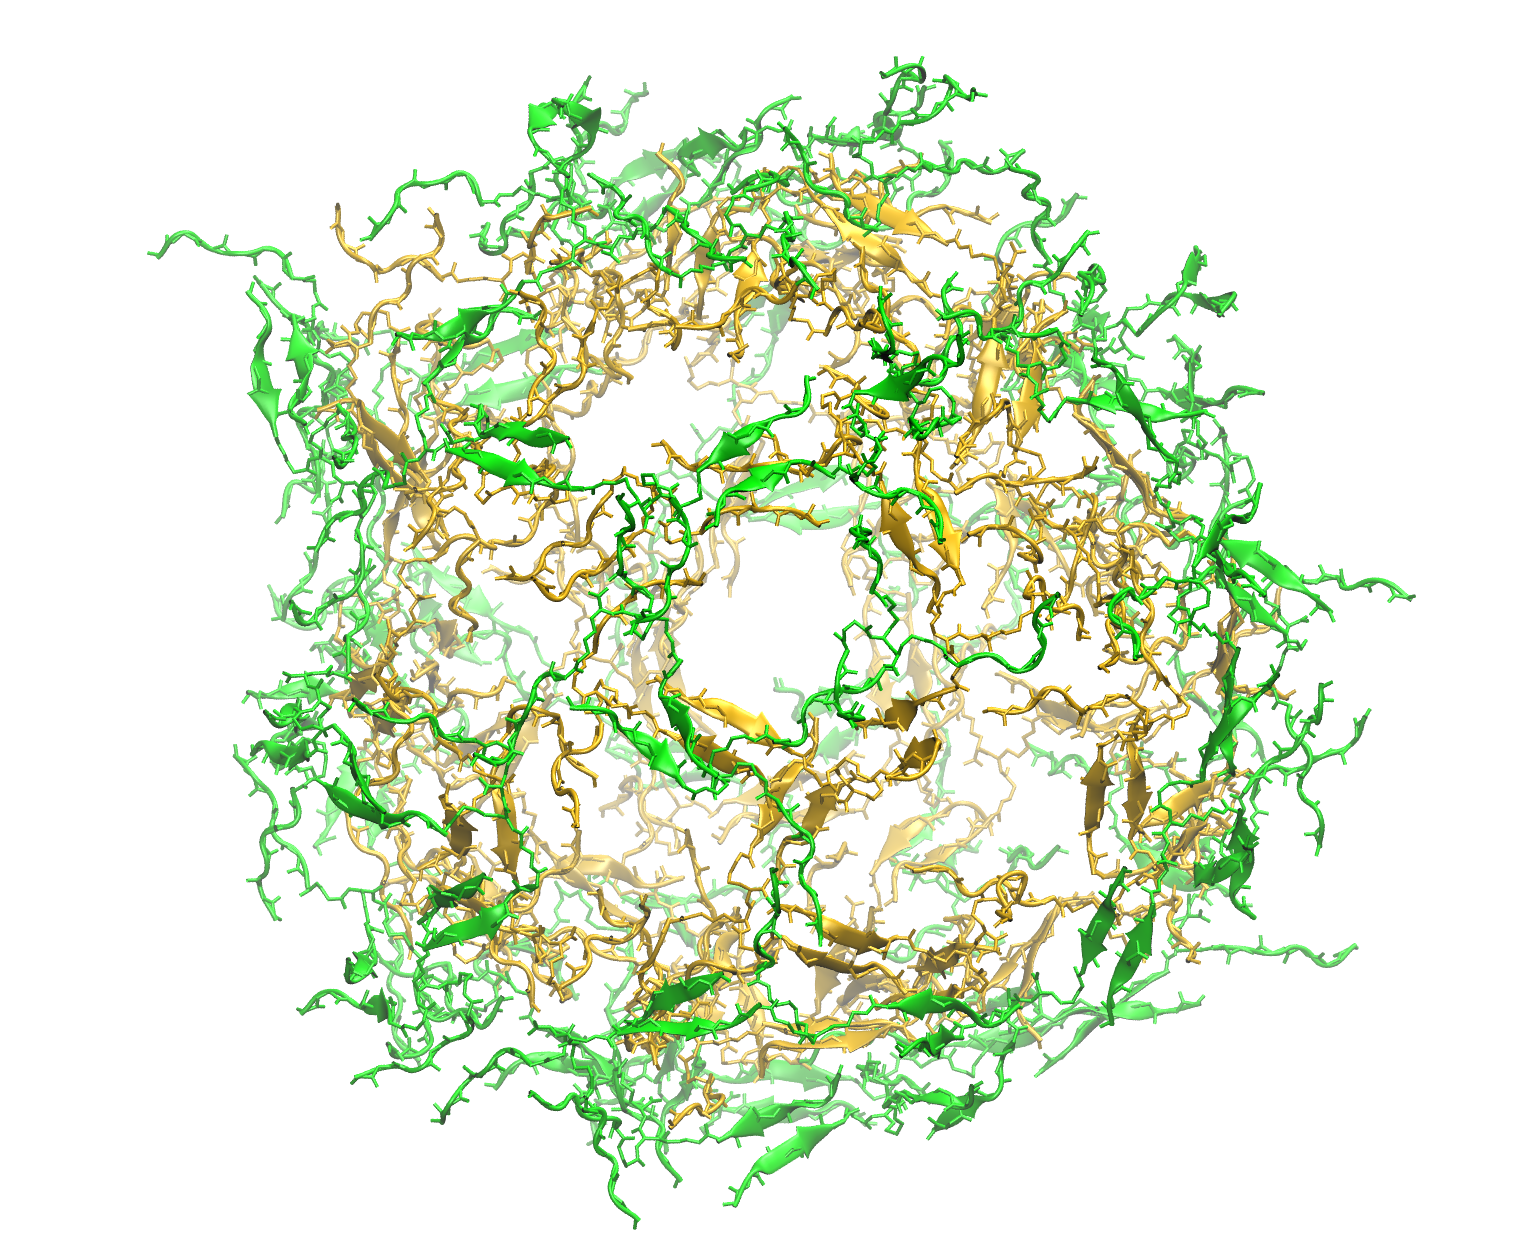
\includegraphics[width=0.5\linewidth]{3results_capsule/pics/staR3_render}
\caption[Atomistic run of buckyball in solution: final configuration]{Final snapshots (100 ns) from the simulation of a buckyball in solution (replica 3): bonds and cartoon representation, backbone only, green external layer and yellow internal one.}
\label{fig:BTI_snap}
\end{figure}

\subsection{Atomistic simulations}

We discuss first the results from atomistic simulations, color coded as black or in shades of grey in the following sections. However, all the plots present back to back the results from coarse grain runs as well, anticipating the discussion of Section \ref{sec:res_multiscale}, as this would make easier the comparison later on.

\begin{figure}[p!]
\centering
\subbottom[]{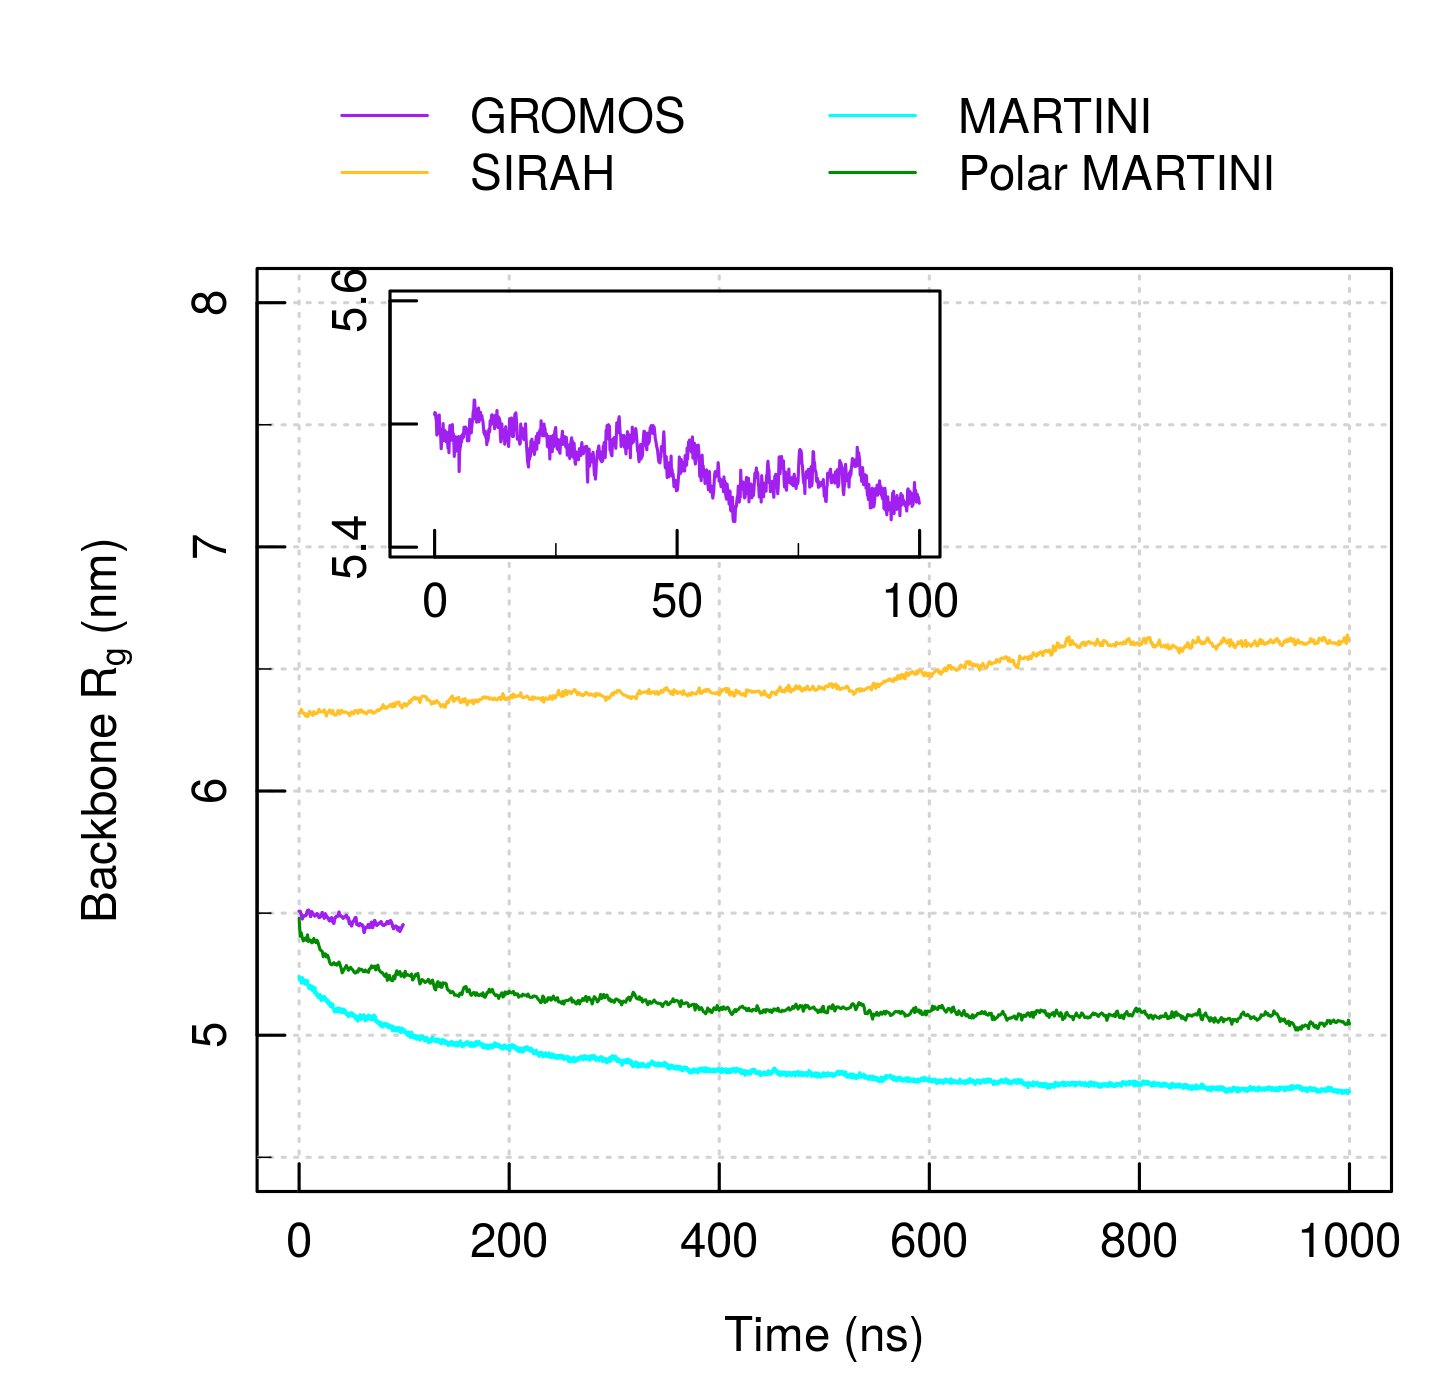
\includegraphics[width=0.48\linewidth]{3results_capsule/pics/Rg_all.png} \label{fig:Rg}} 
\subbottom[]{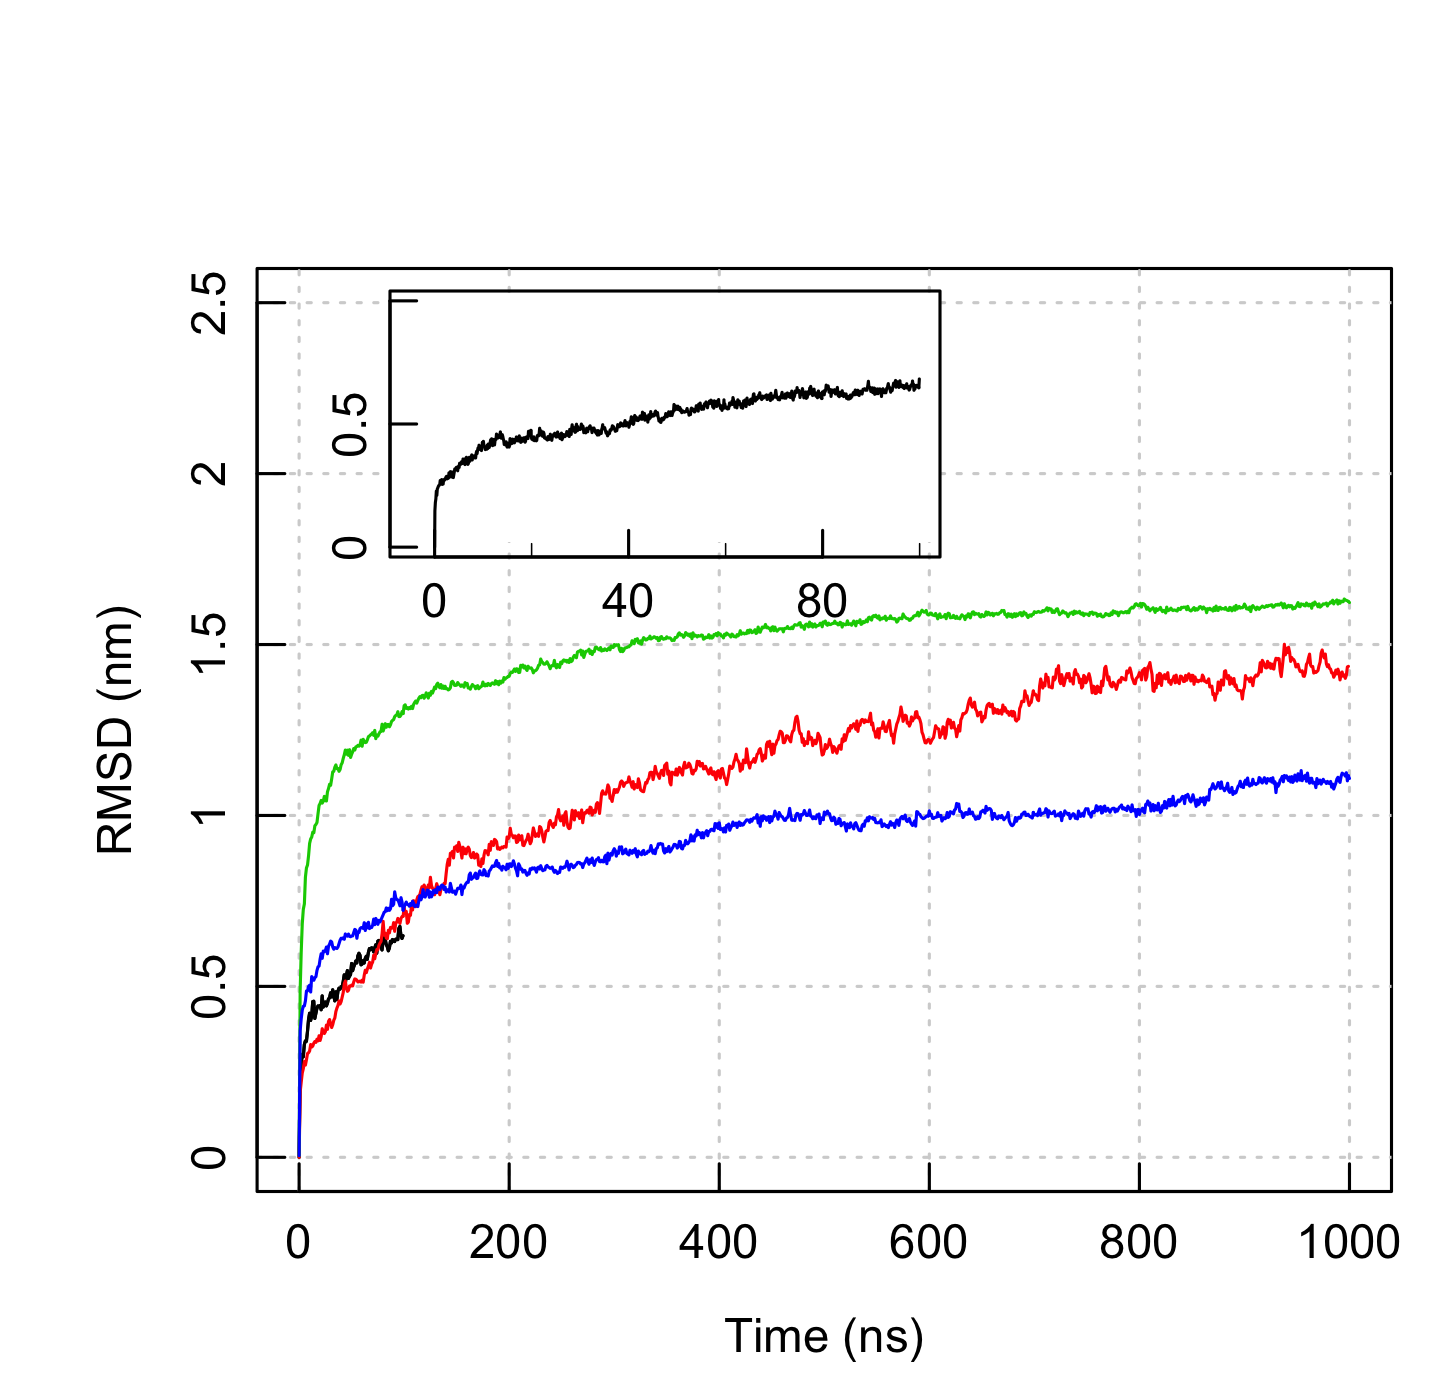
\includegraphics[width=0.48\linewidth]{3results_capsule/pics/RMSD_all.png} \label{fig:RMSD}} \\
\subbottom[]{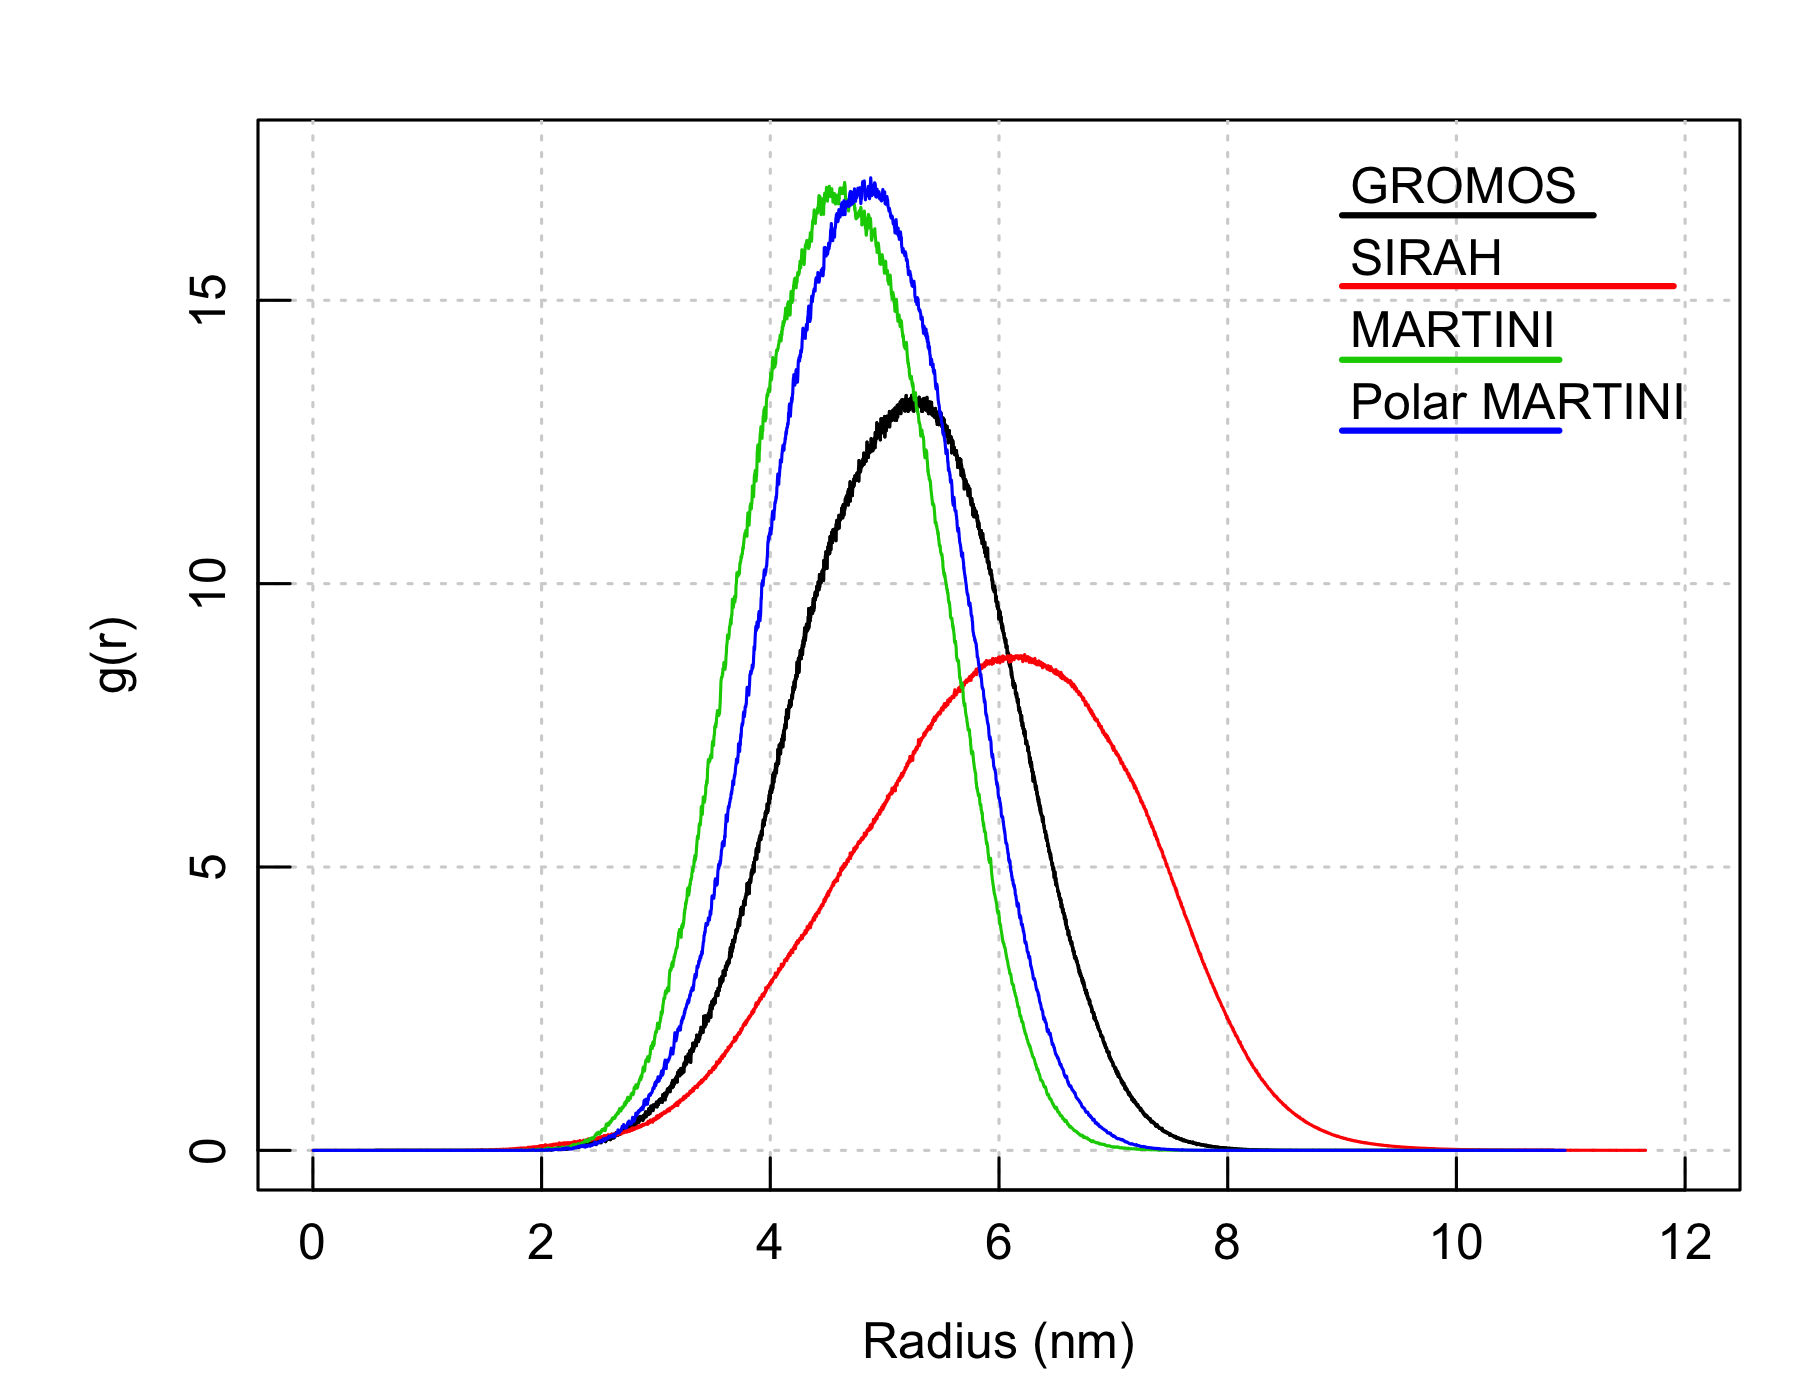
\includegraphics[width=0.6\linewidth]{3results_capsule/pics/RDF_all.png} \label{fig:RDF}}
\caption[Structural measures on buckyball in solution]{(a) R$_g$ and (b) RMSD computed respectively on the Protein and its backbone. Results are displayed for simulations performed in GROMOS (100 ns), SIRAH, MARTINI and MARTINI with polar water (all 1 $\mu$s). Inset: zoom on the GROMOS values. (c) RDF of Protein masses around their center of mass, computed on both layers, displayed for the same simulation set up as in (a,b). For each label of the legend, the bar has length of the respective RDF FWHM (thickness estimate). All results are showed for Replica 1 of each simulation setup.}
\label{fig:struct_UA_SIhere}
\end{figure}
%
\paragraph{Global capsule structure} Atomistic simulations of the buckyball in solution show a consistently equilibrated structure across the three replicas (Figure \ref{fig:BTI_snap} and SI movie --).
%
This is proven by both the stable value of the protein R$_g$ and the almost plateauing backbone RMSD (Figure \ref{fig:Rg} and \subcaptionref{fig:RMSD}). It is interesting to notice that previous simulations performed with a shorter equilibration, without the phase employing flat bottom restraints, resulted in the immediate disruption of several connections in the buckyball network, with resulting larger R$_g$. This suggests that the structural pairing present in the structure can form only when the chains are in close contact. For this to happen, many conformations need to be sampled, and this is compatible with the long time of assembly observed experimentally (up to 7-10 hours).
%
The RDF of the protein masses around the buckyball centre of mass shows a Gaussian profile (Figure \ref{fig:RDF}). The fact that no masses are observed nearby the origin means that the molecules do not collapse to the center and the central cavity is maintained. To be noticed that, given the way RDF is computed and normalised, a uniformly full object would display a flat distribution.
%
A fit of the RDF to a Gaussian curve returns a mean value of 5.1 nm and a FWHM of 2.2 nm, which gives an estimate of the bilayer thickness.
%
A similar computation is repeated for the inner and outer layer separately, providing 1.1 nm of distance between the two distributions means. This interlayer distance is compatible with the distance between the backbones of stacking $\beta$-sheet in structures like densely packed amyloids with cross-$\beta$ sheet quaternary structure (1.0 nm \cite{Sunde1997}).

\begin{figure}[p]
\centering
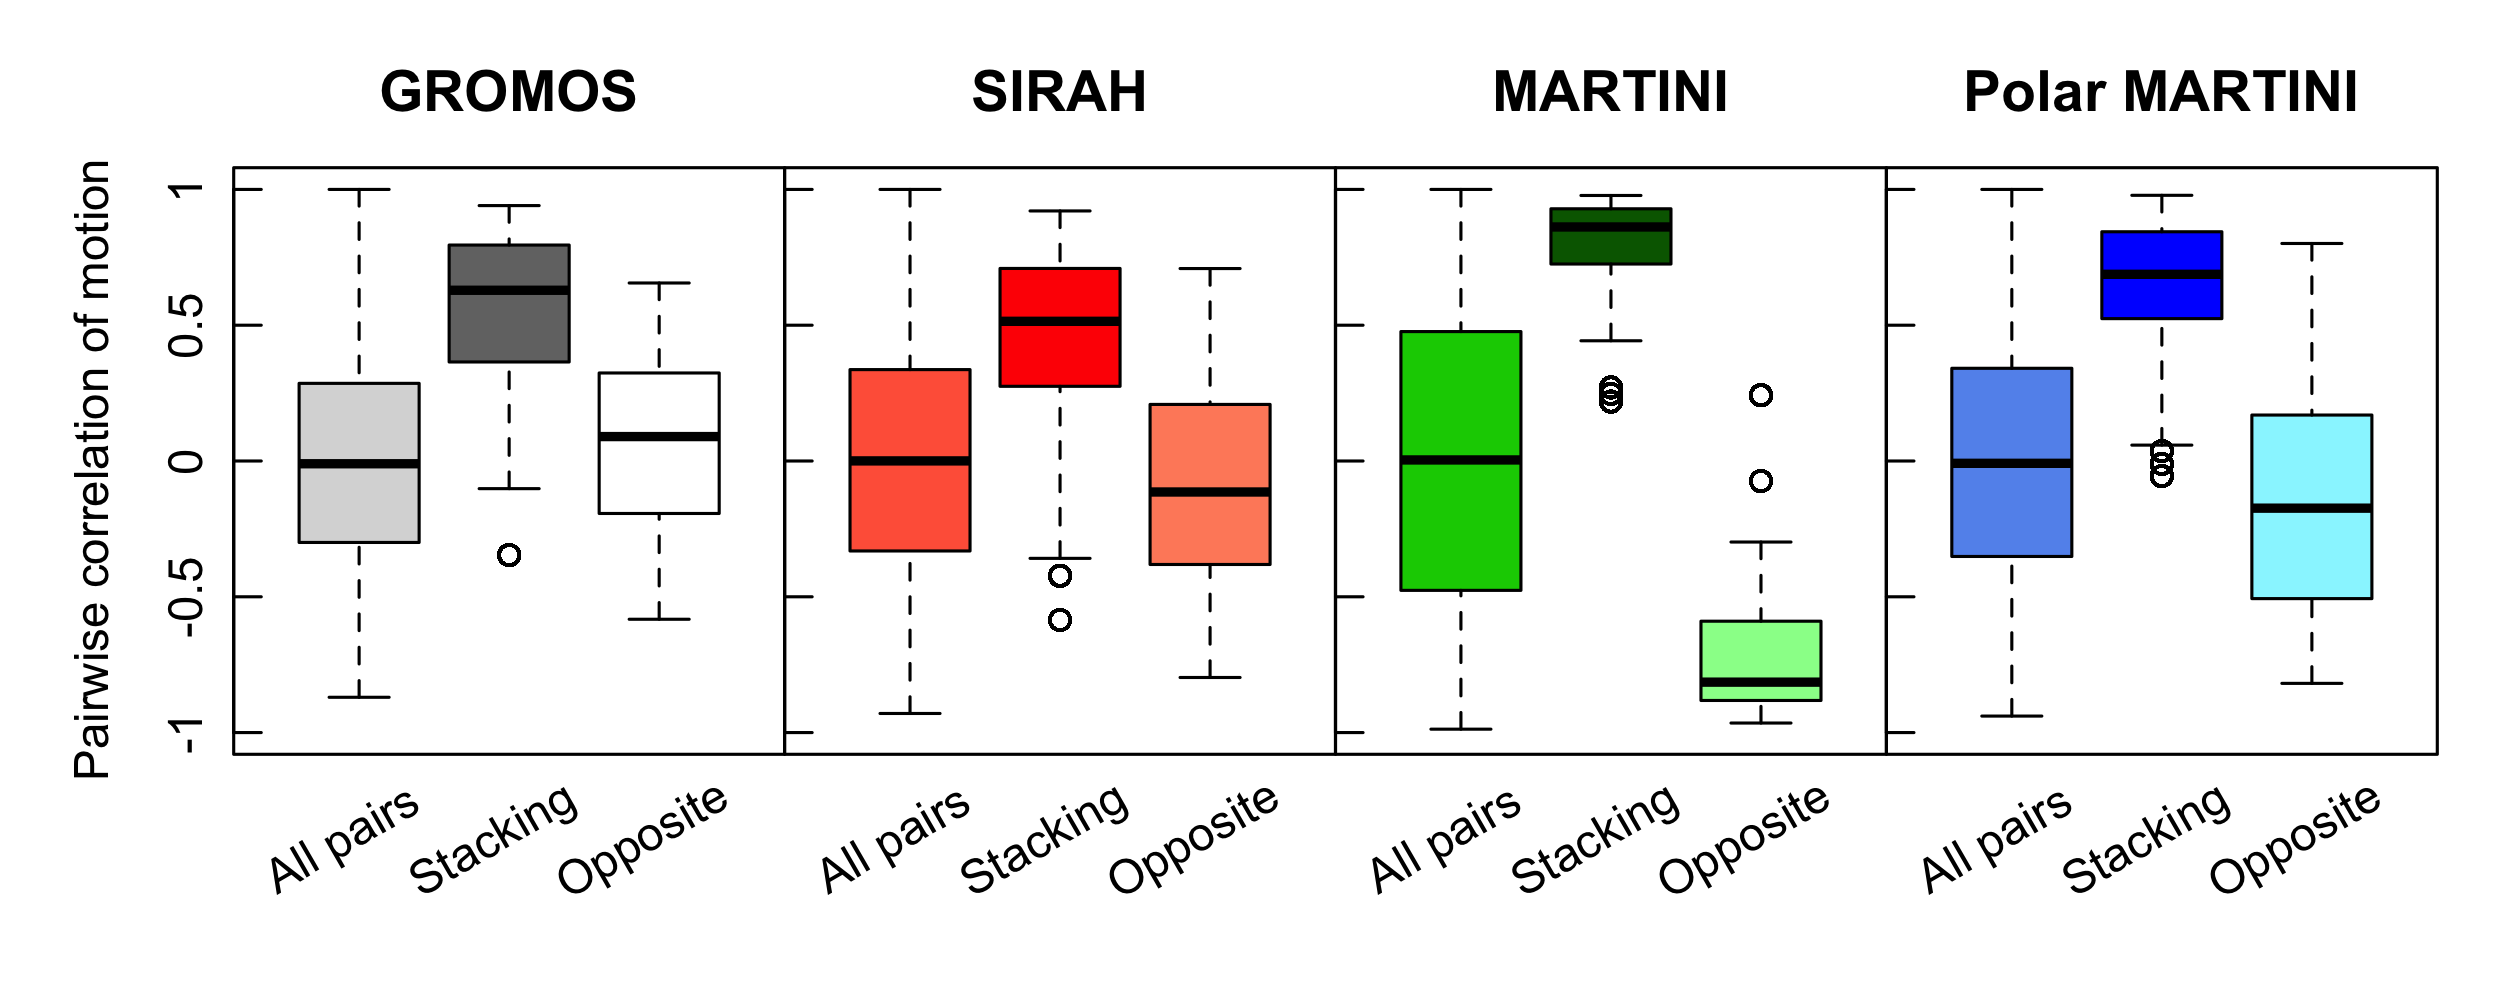
\includegraphics[width=0.95\linewidth]{3results_capsule/pics/RKGBcorr_boxplot_all.png} 
\caption[Correlation of motion between molecules of the buckyball]{Distribution of the correlation of motion between different molecules in the buckyball simulations. Black band: median of the distribution; box: first and third quartiles; whiskers: maximum and minimum, outliers excluded (hollow dots). Results are shown for Replica 1 of each simulation setup.}
\label{fig:BTI_corr}
\end{figure}
%
This thickness value hints at the fact that the two layers are closely packed. This is confirmed by the analysis of the pairwise correlations of motion:
%
molecules at the same polar coordinates (i.e. stacking radially one on the other) have a positive correlation and so move coherently, while the ones at opposite poles, as well the ensemble of all possible pairs, do not show particular correlation (Figure \ref{fig:BTI_corr}). 

\paragraph{Contacts between molecules} The measure of paired branches in the buckyball network, shown in Figure \ref{fig:BTI_beta}, reports an average (in time) of 240 pairings between arms belonging to the same layer (summing over inner and outer), four pairing per molecule, and around 60 only for inter-layer ones.
%
\begin{figure}[p]
\centering
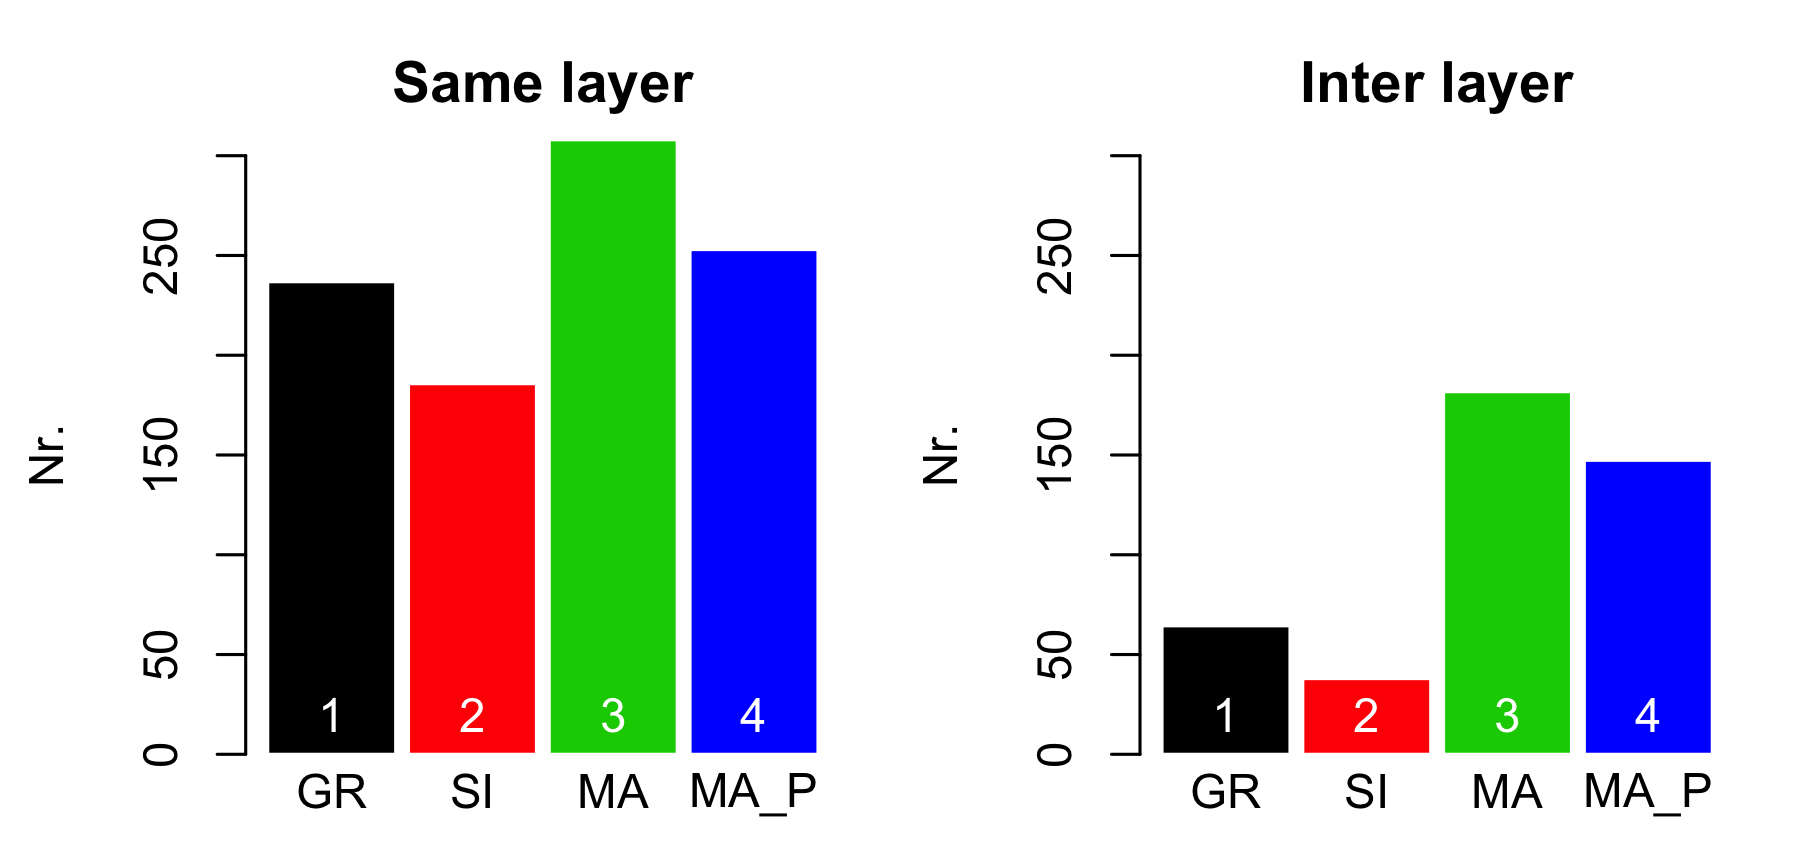
\includegraphics[width=0.85\linewidth]{3results_capsule/pics/stAll_beta_R1.png}
\caption[Branch pairing during simulations of the buckyball]{\textbf{[RECOMPUTING]} Number of paired branches within the same layer and between layers, as defined in the main text. Results are shown for Replica 1 of each simulation setup.}
\label{fig:BTI_beta}
\end{figure}
%
This first value is larger than the one predicted for a perfect buckyball arrangement (which would be three), likely due to the fact that the structure contracts slightly with respect to the initial size and some branches deviate from the original position, locating themselves in the proximity of multiple neighbours. On the contrary, few inter layer contacts are observed within 1.2 nm distance cut off because of the steric hindrance of the side chains which are located in between the two layers, as they keep the average position of inter-layer backbone stretches at a distance greater than the cut off chosen.

\begin{figure}[p]
\centering
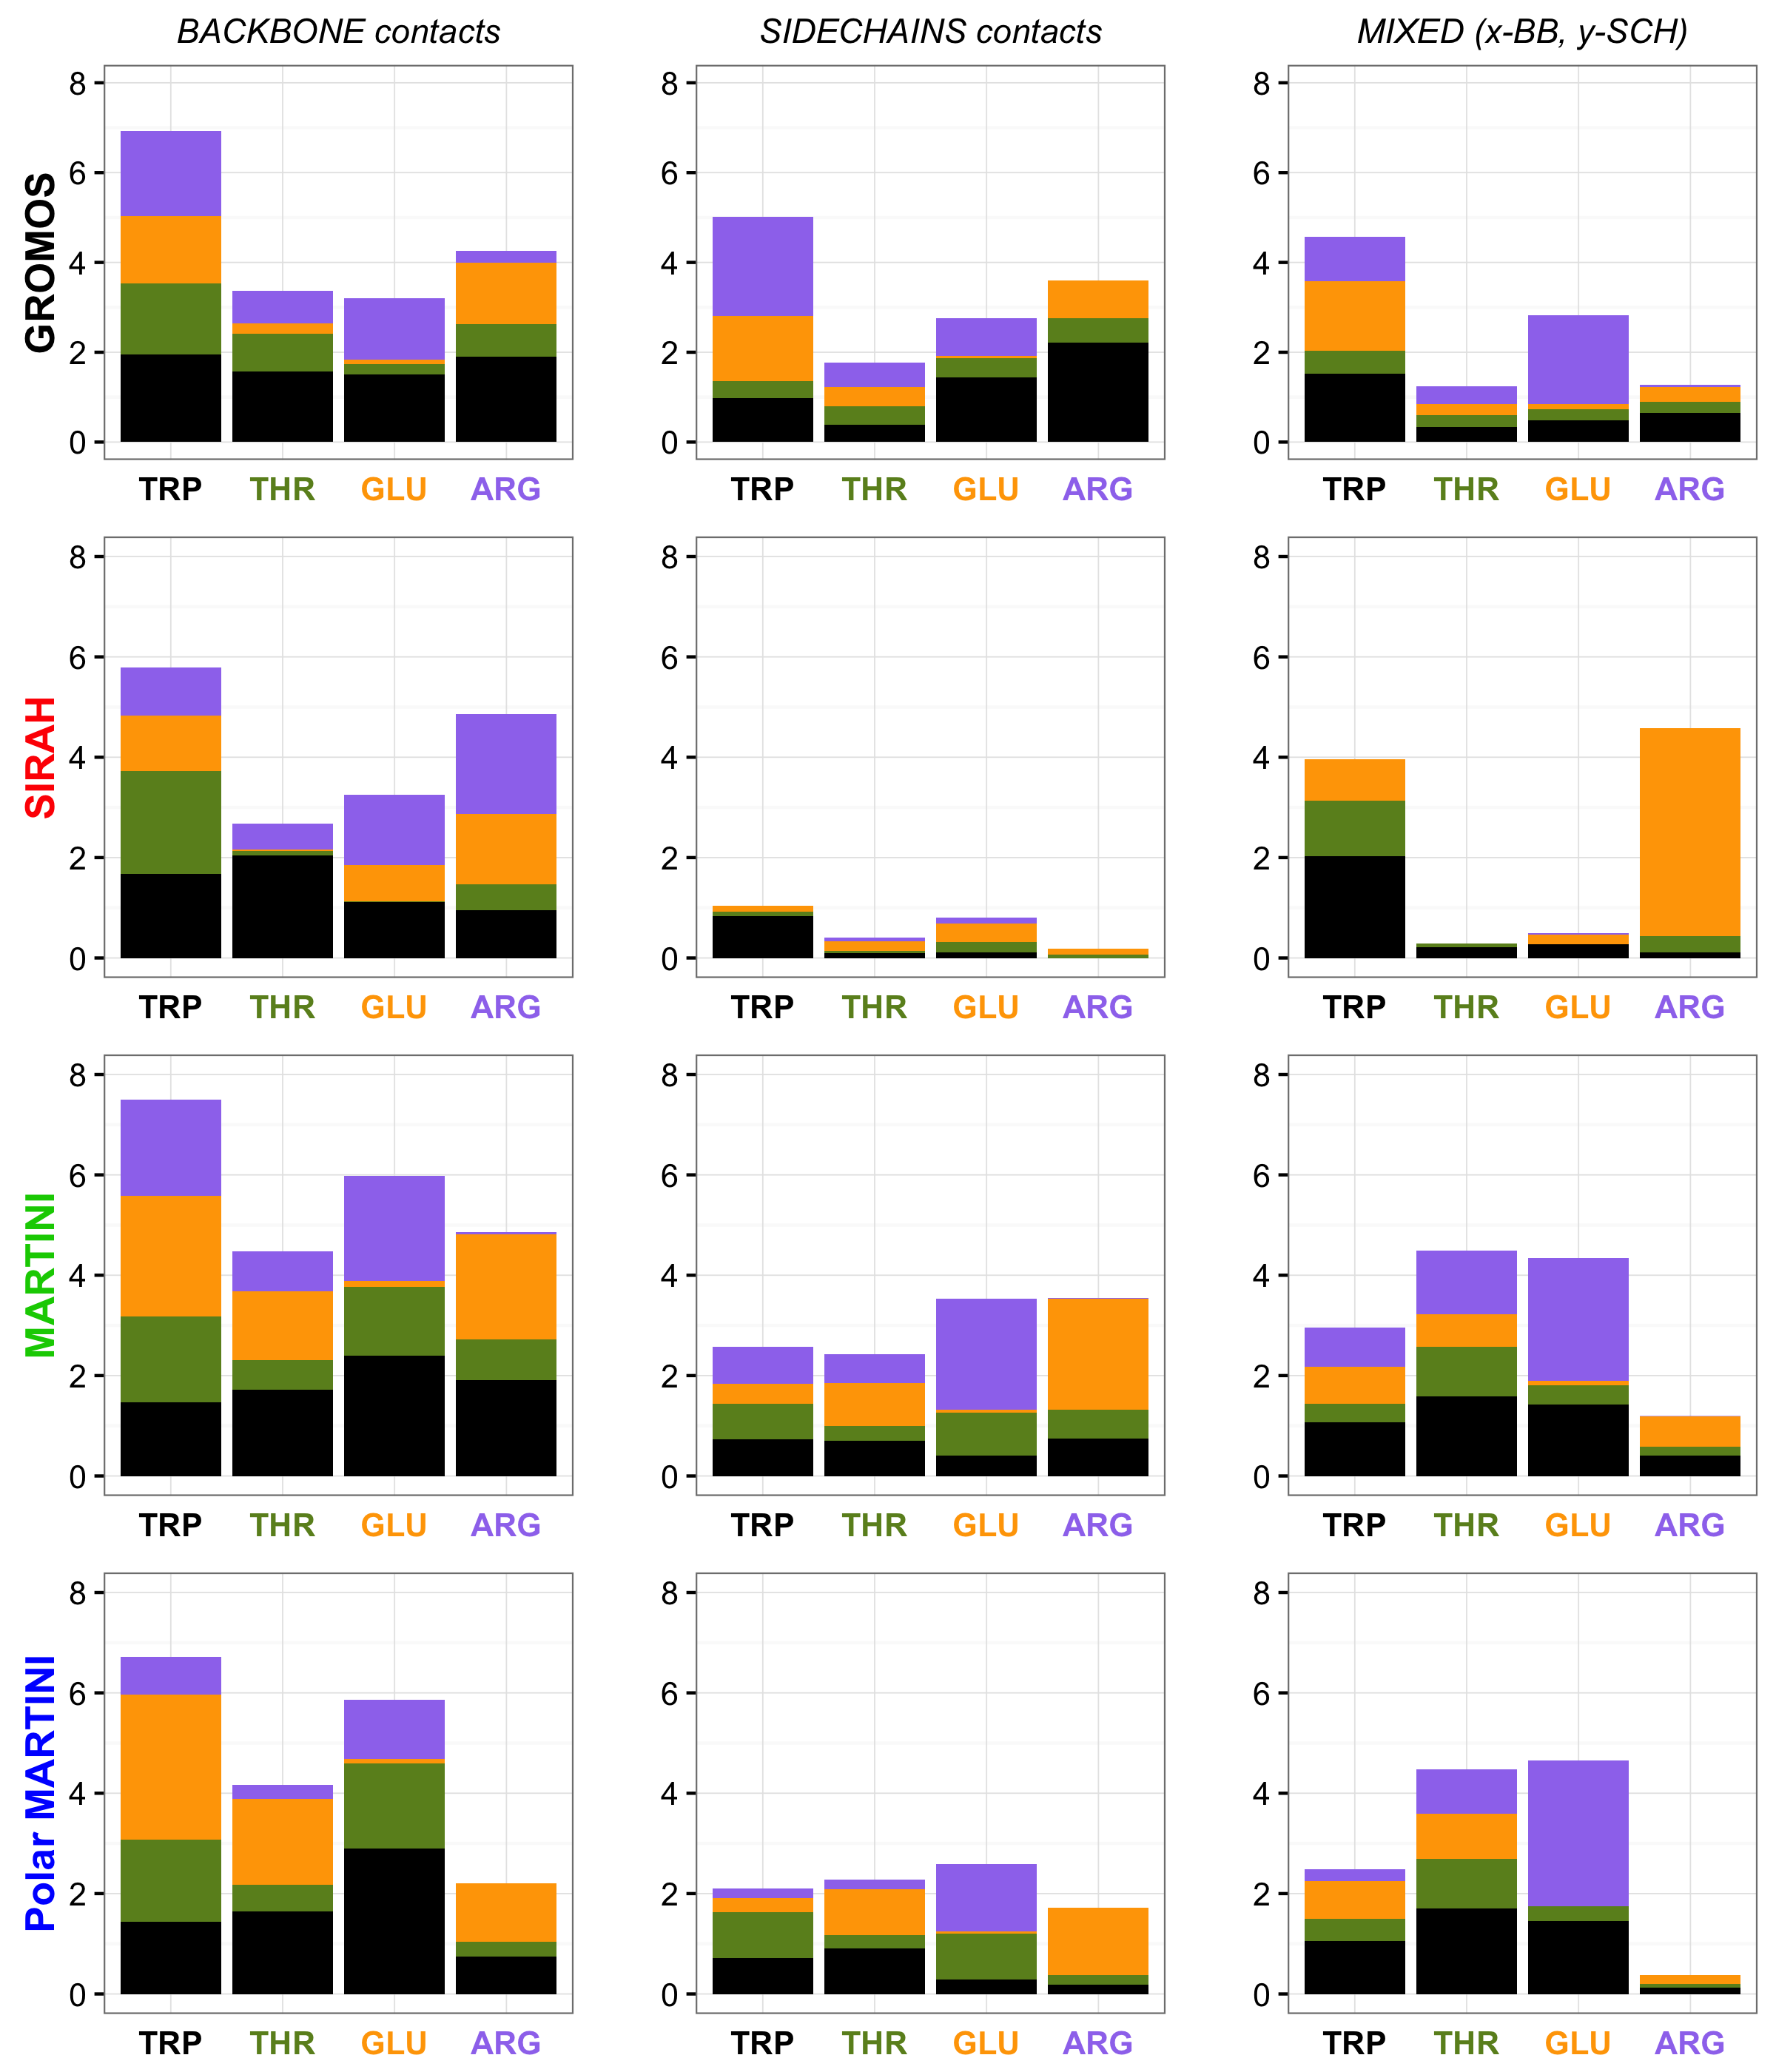
\includegraphics[width=0.95\linewidth]{3results_capsule/pics/new_rep1_allFF.png}
\caption[Contacts between molecules during simulations of the buckyball]{Contacts with persistence greater than 50\% between C$_\alpha$s (Backbone contacts), between side chains (Sidechain contacts) and mixed (in which case, for each bar, the residue on the $x$-axis contributes to the contact with its backbone, and the bar is split by the identity of the partner engaging its side chain). The simulation setup is reported along the $y$-axis. Results are shown for Replica 1 of each simulation setup.}
\label{fig:BTI_cont}
\end{figure}

To look more into the details of the interactions between arms of the molecules, we computed the contacts between backbone and/or side chains of amino acids, normalised by the number of molecules present, and classified the ones which survive more that 50\% of the simulation time by residue type (Figure \ref{fig:BTI_cont}). 
%
The number of backbone contacts per molecule is around 3 for Threonine, Glutammic acid, 4 for Arginine, and between 6 and 7 for Tryptophan residues.
%
As in each molecule there are 3 Threonine and 3 Glutammic acid but 6 Arginine and 6 Tryptophan, this proves that on average each residue is well paired with another one, except for Arginines: only two thirds of them are paired on average, likely because of their terminal position.
%
At the same time however the bar plot shows also that there is no rigid arrangement between branches. Indeed, for example, Tryptophan residues are not chiefly paired to Tryptophan ones, as the optimal arrangement would be, suggesting flexibility in the structure.
%
Nevertheless, the analysis highlights that Trp residues are key to form contacts with the neighbours and (from the central column) that their cation-$\pi$ interaction with Arginine through their side chains is an important element of the structure.

\paragraph{Hydrogen bonds interaction} Some of these contacts are mediated by an hydrogen bond interaction: the number of them present during the simulations is computed, and divided by the number of molecules.
% SAY THAT THEY ARE THE ONE OCCURRING AT ANY MOMENT, AND NOT THE ONES SURVIVING MORE THAN 50%?
We classify the hydrogen bonds occurring between backbones and/or side chains of the amino acids, breaking them by amino acid type. Tryptophan contributes to a large number of backbone hydrogen bonds (Figure \ref{fig:BTI_hbonds} top), especially with other Tryoptophan residues, consistently with what found in the analysis of contacts carried on above. Arginin side chains are the most prone to establish H-bonds as a donor with many different amino acid side chains, but especially with Glutammic acid as expected from the facing positions they occupy in the molecules arrangement.
%
\begin{figure}[t]
\centering
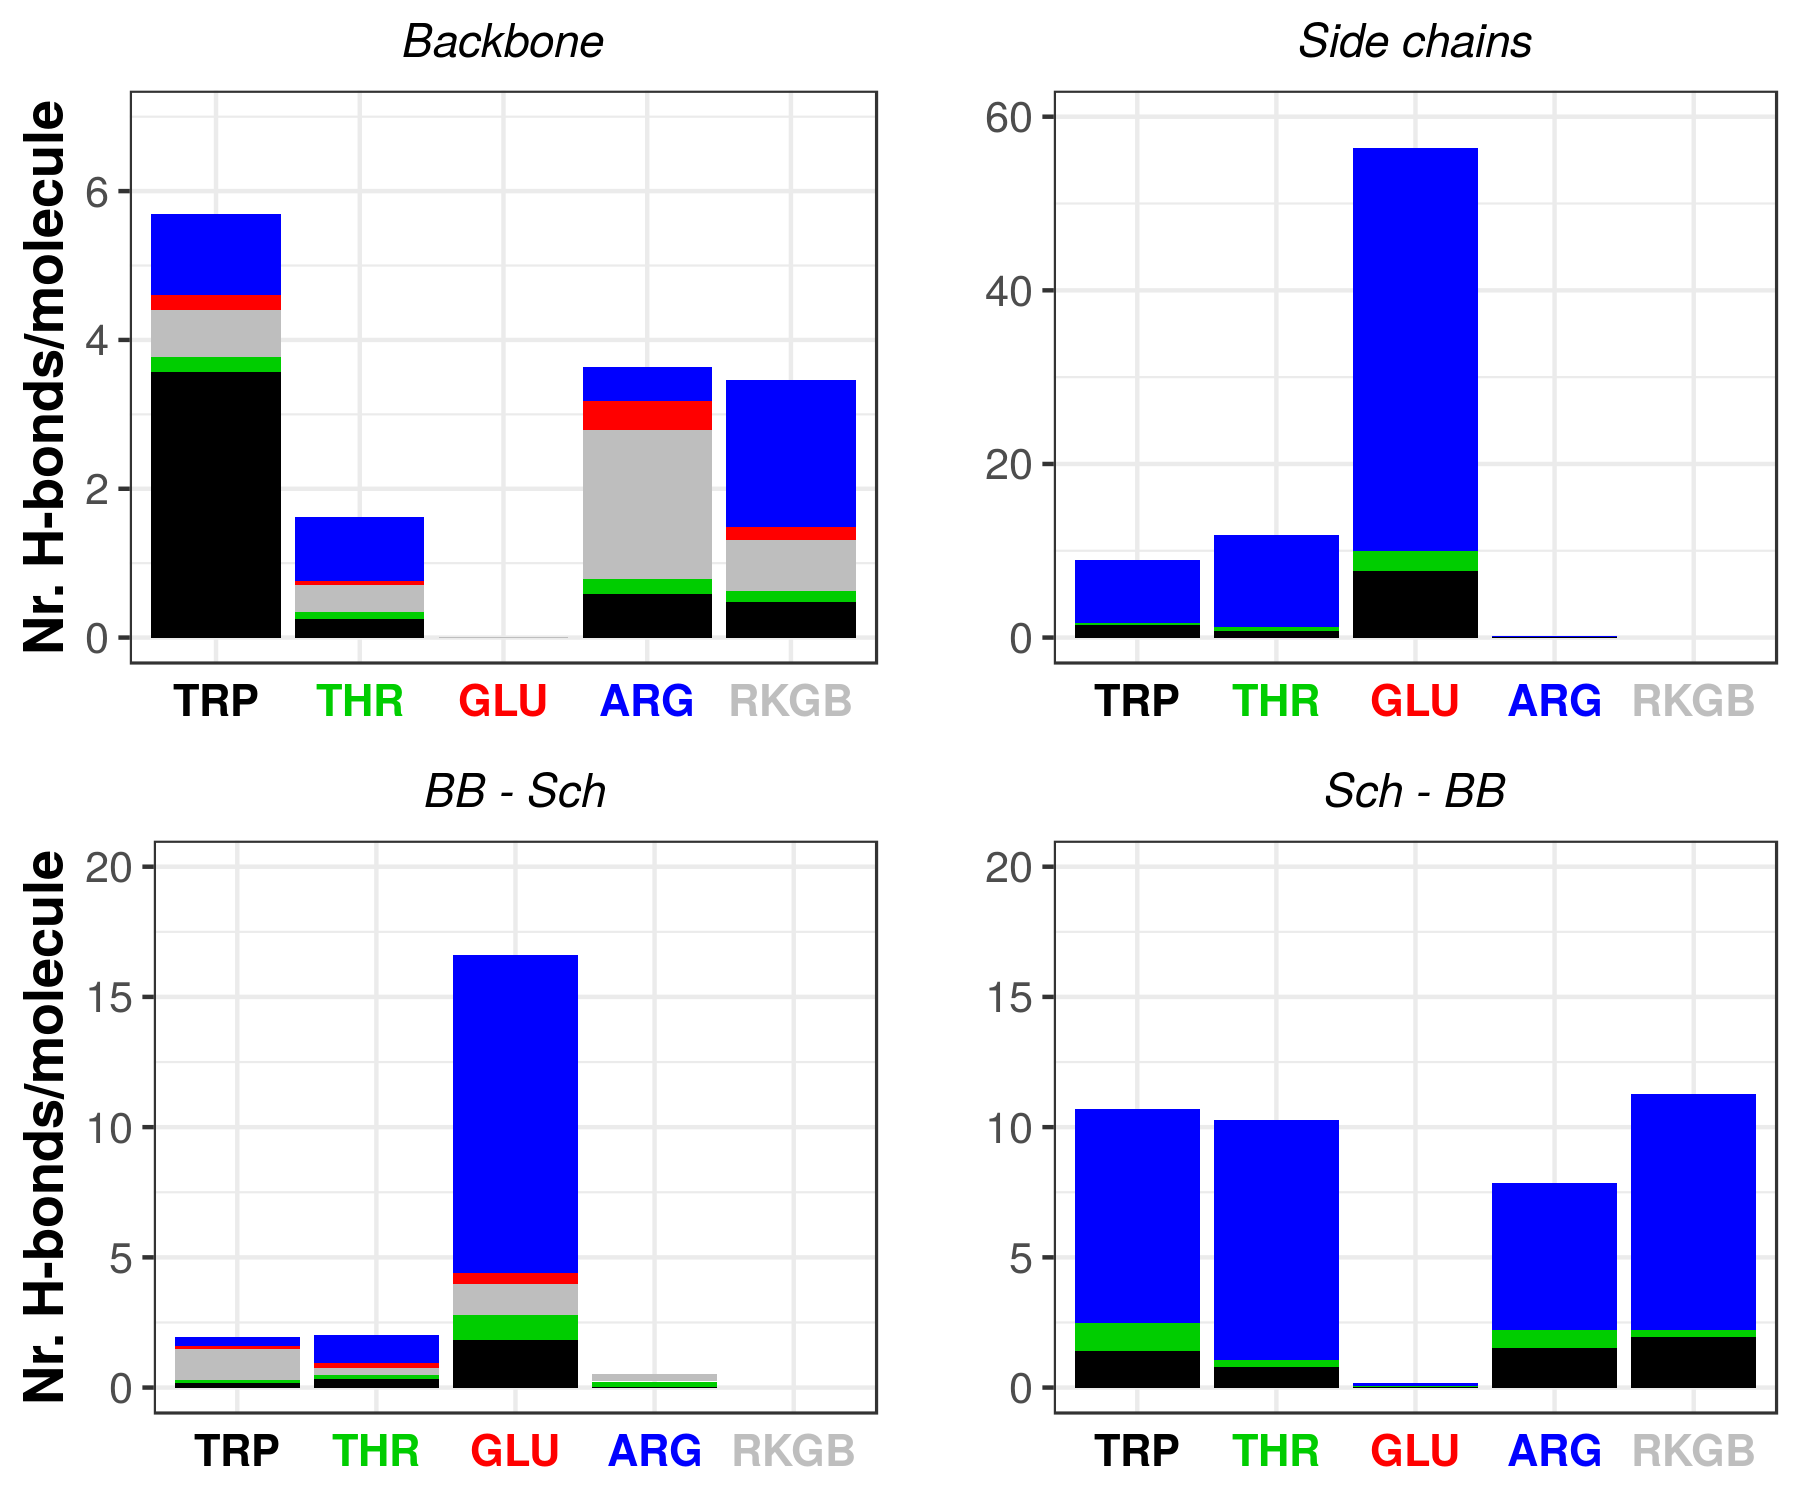
\includegraphics[width=0.85\linewidth]{3results_capsule/pics/Hb_all.png} 
\caption[Hydrogen bonds in the buckyball molecule]{Average number of hydrogen bonds per molecule occurring between amino acids, including the central scaffold RKGB, in a 100 ns atomistic simulation of the buckyball in solution. Result are shown for Replica 1. For each bar, the residue on the $x$-axis is the acceptor, and the bar is split by the identity of the donors. In the case of Backbone - Side chain and Side chain - backbone, the first mentioned correspond to the acceptor (and thus the residue on the $x$-axis).}
\label{fig:BTI_hbonds}
\end{figure}

\paragraph{Chemical characteristics of the surface: SASA} Finally, it is important to understand what residues are exposed at the surface of the structure, especially in view of future applications: in order to make the peptide co-assemble with other products, the two must have a compatible chemical character. To understand what surface the peptide exposes to the solution, we compute the average Solvent Accessible Surface Area (SASA) per molecule and break it down by amino acid type. Figure \ref{fig:BTI_sasa_exposed} shows that half of the accessible surface is represented by the charged residues Arginine, while Tryptophan contribute to less than one quarter to it, despite having bulky side chains. For atomistic simulations, we can compare the SASA per each residue X, with the reference SASA computed on simulations of a Gly-X-Gly tripeptide (computation performed with the software POPS \cite{pops}). The resulting ratio $Q_{SASA}$ is greater than one for both the Arginines: while for the terminal one (ARG1) it is suspected, the fact that also the second has $Q_{SASA}>1$ proves that these residues are highly exposed in solution. On the contrary, all the other residues have values around $0.5$: for Tryptophan this is due to their propensity to be buried inside the structure, while for Glutammic acid and especially Threonine, despite having charged or polar side chains, they are shielded from the solvent by the large Trp side chains nearby them.
%The screening of the hydrophobic residues is a consequence of the double layer structure and it is crucial in the perspective of binding mechanisms to membranes, in particular to the anionic bacterial one.
\begin{figure}[t]
\centering
\subbottom[]{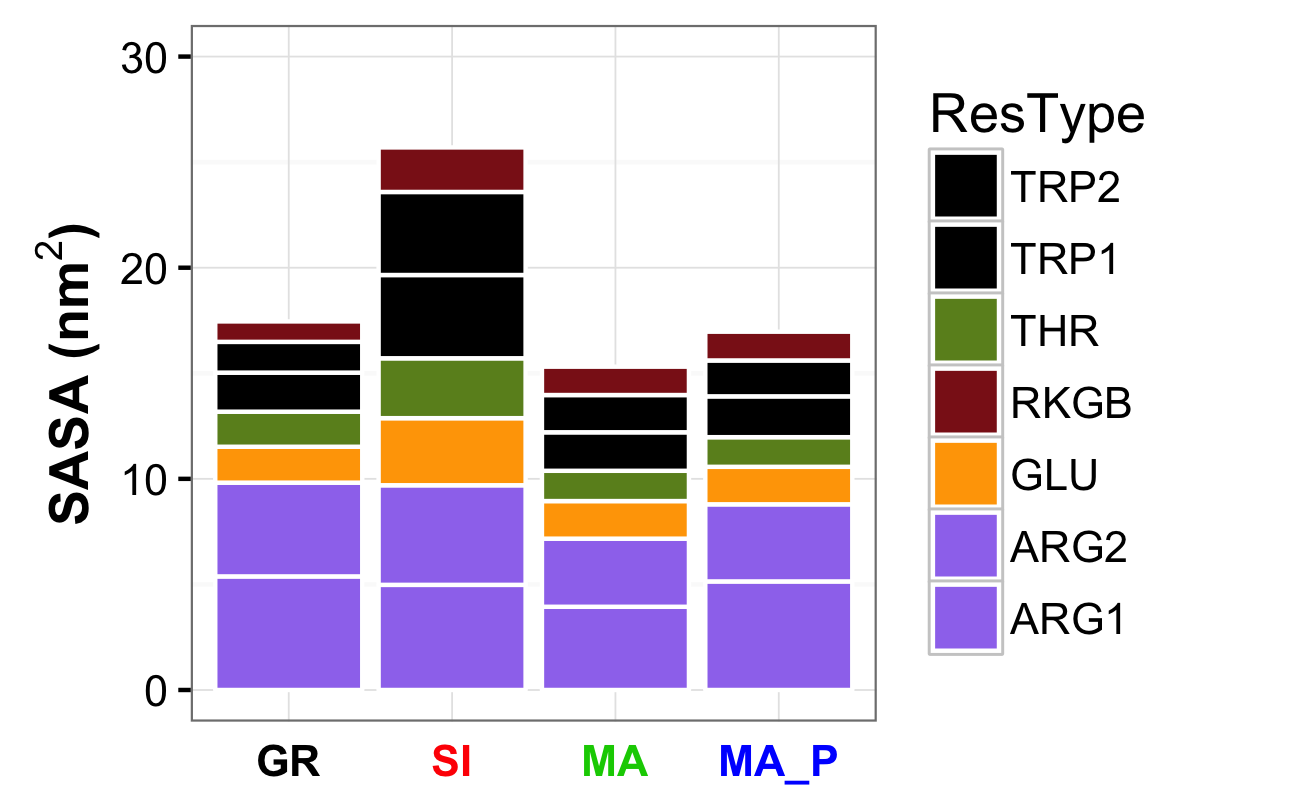
\includegraphics[height=0.3\linewidth]{3results_capsule/pics/st_All_sasa_fractions.png} \label{fig:all_sasa}} 
\subbottom[]{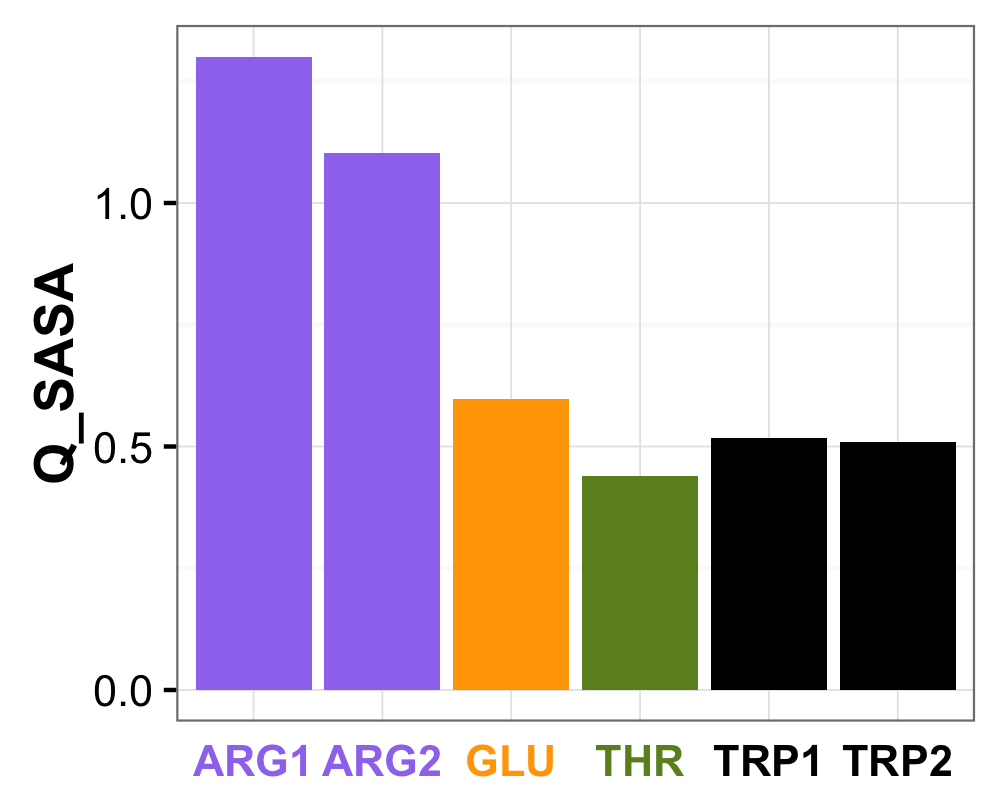
\includegraphics[height=0.3\linewidth]{3results_capsule/pics/st_All_Qsasa.png} \label{fig:Q_sasa}} 
\caption[SASA per residue of a buckyball in solution]{(a) Break down of the Solvent Accessible Surface Area (SASA) per molecule by residue types. Results are shown for Replica 1 of each simulation setup. (b) Normalised SASA over the reference SASA computed for each amino acid type X as the value in a Gly-X-Gly tripeptide.}
\label{fig:BTI_sasa_exposed}
\end{figure}


\subsection{Multiscale comparison of model capsule} \label{sec:res_multiscale}

We performed a multiscale analysis of the capsule structure simulating it with different coarse grain force fields, with a twofold aim: first we wanted to simulate the assembly for a longer time, to observe how its structural properties are maintained on the medium time scale (of the order of the microsecond). Second, we believe that proving the stability of the capsule with different descriptions strengthens the evidence that the assembly proposed is indeed a favourable arrangement of the molecules in solution.

As mentioned before, to this aim we compared simulations run with the SIRAH, MARTINI force fields and MARTINI used in conjunction with polar water. The investigation is also useful to compare how the different descriptions differ and to infer the advantages of each model.
%
We first comment on the quantities already analysed at the atomistic level (if applicable), and then extend the analysis to simulations of a monolayer capsule, which has been modelled to prove the greater stability of the bilayer one.

\paragraph{Force field comparison}
As foreseeable, the structures obtained with coarse grain force fields are slightly different with respect to the atomistic one and among themselves.
%
The SIRAH simulated bilayer capsule has a more open structure with respect to the atomistic one, with a skewed and broader radial density profile, while MARTINI with the standard water model provides a more compact configuration (respectively 6.0 nm and 4.6 nm average radius, with 2.9 nm and 1.9 nm average thickness - see Figure \ref{fig:Rg} and \subcaptionref{fig:RDF}). MARTINI with polar water provides a slightly larger structure with respect to standard MARTINI (4.8 nm average radius), with a comparable thickness. This is likely due to the poorer properties of solvation of standard MARTINI water, which cause the protein beads to preferentially interact between themselves rather than with the solvent. 

The correlation of motion between molecules for all the coarse grain force field is similar to the results of the atomistic one, with a slight anticorrelation between molecules at the opposite poles (Figure \ref{fig:BTI_corr}). This is due to the contraction or expansion happening at the beginning at the simulation, when the capsule adjusts to the equilibrium size, which depend to some extent on the force field.
%
These effects though are slightly more pronounced for the MARTINI force fields, probably due to the greater cohesion between the beads which makes them moving coherently.

% CONTACTS:
%			GR		SI		MA		MAP
% SAME		234		179		138		246
% INTER 		62	    42   	171		128
The number of chain paired in the SIRAH simulations is fewer than in the atomistic ones (Figure \ref{fig:BTI_beta}), in line with a more expanded structure, while MARTINI simulations propose a higher number, consistently with the reduced size of the capsule. In particular, the inter layer contacts are consistently higher, as would be expected when the two layers are closer and more strongly bound, as suggested by the values of the stacking molecules correlation. Finally, there is little difference between MARTINI and Polar MARTINI in this measure.

Breaking down the contact analysis by residue type (Figure \ref{fig:BTI_cont}), coarse grain simulations shows necessarily a different organisation, due to the fact that different parametrisation results in different proportions between the side chains volumes of different amino acids. Never the less, in all the representations, Tryoptophan has a prominent role in establishing contacts with its neighbours at the backbone level, while different force field suggest different role of the side chains. Quite surprisingly, the SIRAH force field does not promote interactions between side chains a part from the Tryptophan ones with themselves. This seems due to the more expanded structure of the capsule and the larger solvation of the amino acids, which are more exposed in solution (see next paragraph discussing SASA values).
%
Moreover, none of the coarse grain descriptions seem to capture the preferential cation-$\pi$ interaction between Arginine and Tryptophan.

Finally, the values of SASA cannot be compared between force fields, because of the different dimensions and number of atoms/beads employed. However, it is interesting to notice that consistently across force fields, Arginine constitute around half of the exposed surface, with the exception of SIRAH, where the more open structure results in other residues to be more exposed as well (Figure \ref{fig:all_sasa}).

Overall, these results suggest that every coarse grain force field has a particular propensity for an equilibrium distance between peptidic components due to the different property of solvation of the water model chosen. To better understand this, we computed the Coulomb and Lennard-Jones contribution to the energy due to peptide-peptide interactions or peptide-solvent ones.
%
Figure \ref{fig:value_eng_cg} plots these value for the second half of the simulated time for each coarse grain force field (to be noticed that for the SIRAH description the Protein-Protein terms include both the short range interactions and the 1-4 interactions, i.e. the ones computed between atoms separated by three bonds. These interactions are not part of the force field for MARTINI models, so only the short range ones are accounted in those cases).

\begin{figure}[p!]
\centering
\subbottom[]{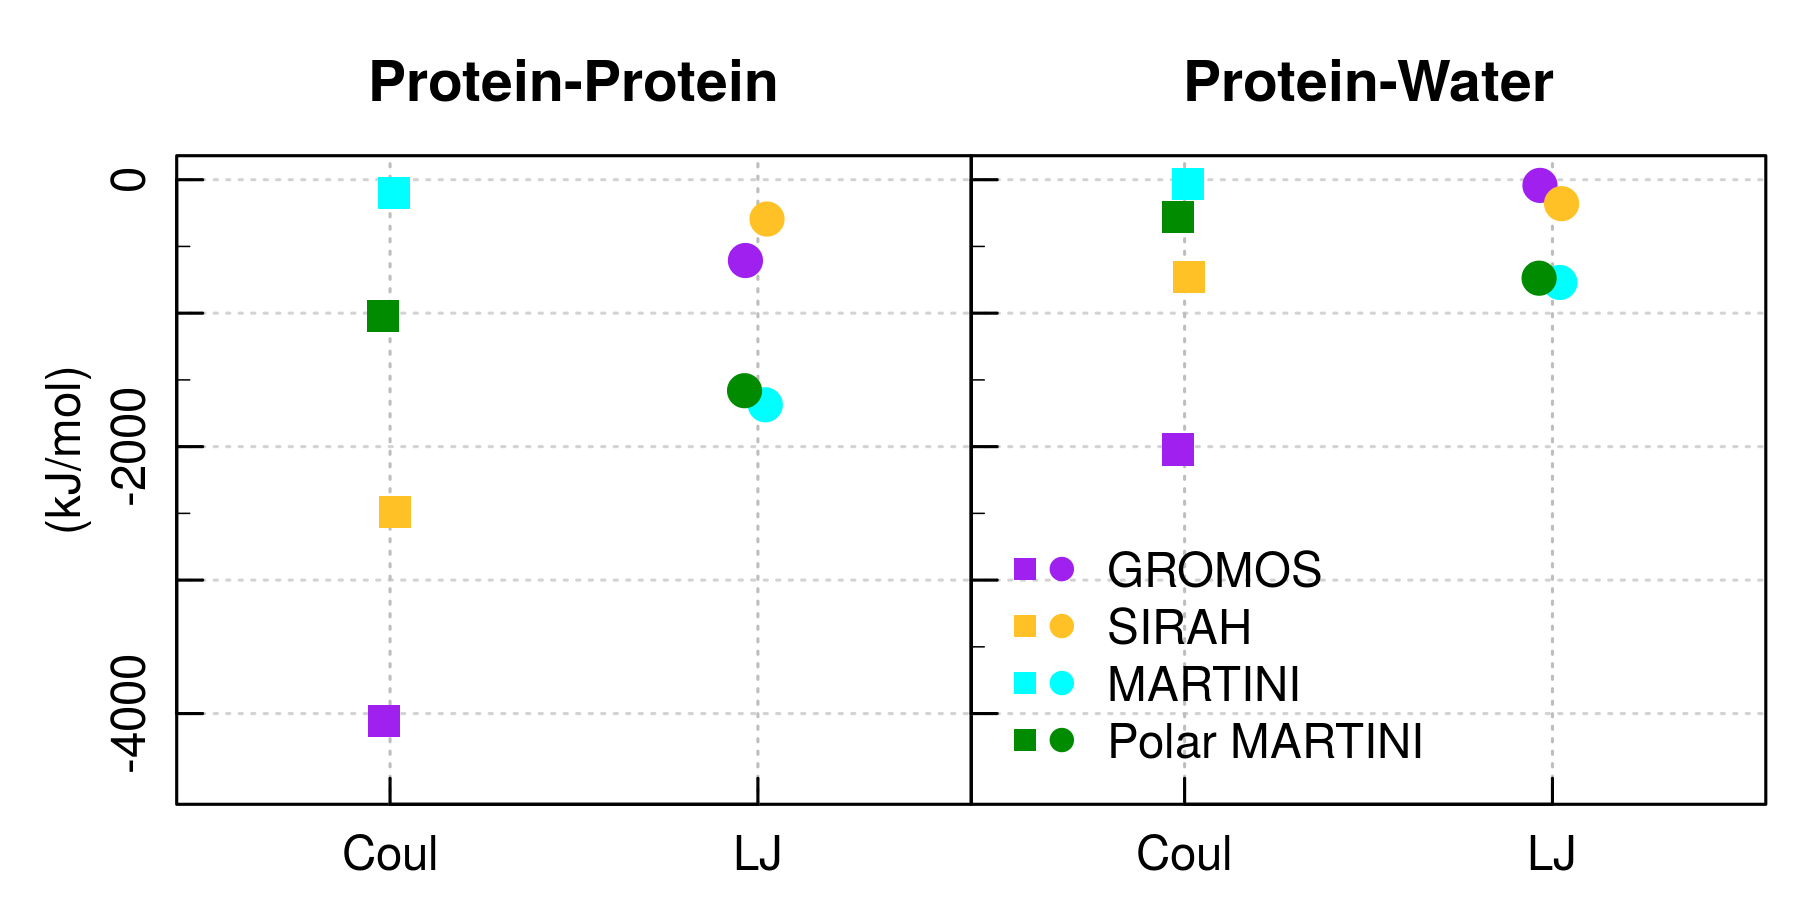
\includegraphics[width=0.8\linewidth]{3results_capsule/pics/many_energies_brief.png} \label{fig:value_eng_cg}} 
\subbottom[]{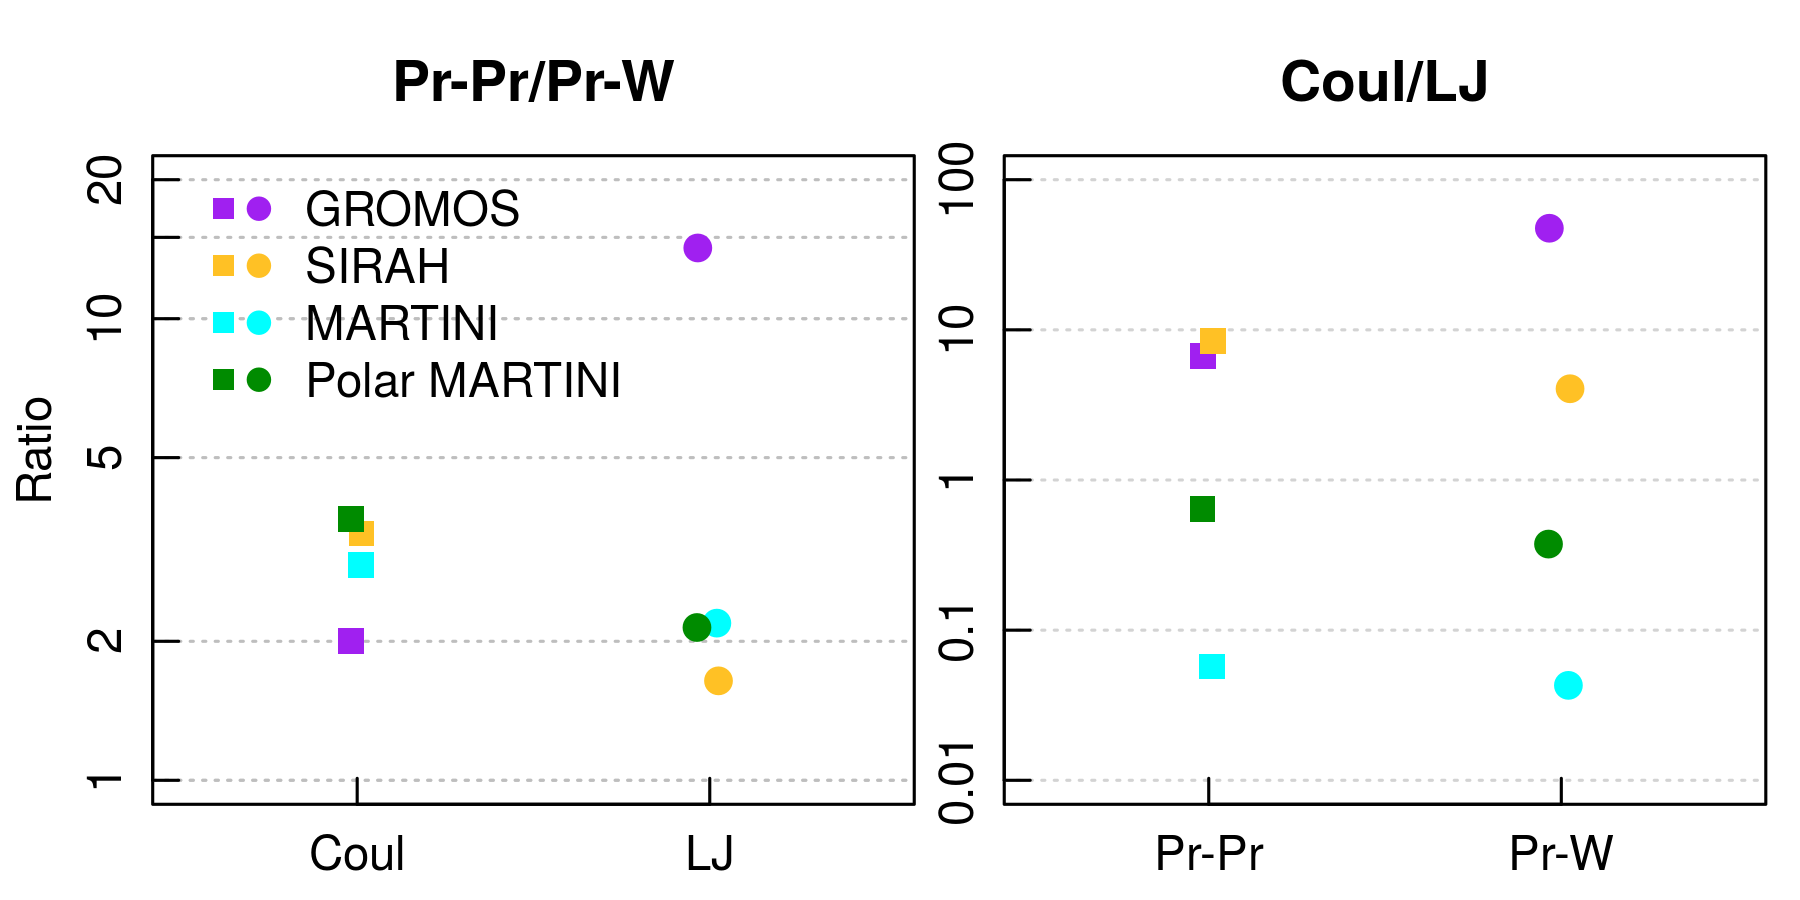
\includegraphics[width=0.8\linewidth]{3results_capsule/pics/ratio_energies_brief.png} \label{fig:ratio_eng_cg}} 
\caption[Non-bonded protein energy contribution to capsule structures]{(a) Protein-Protein and Protein-Water non-bonded interactions, normalised per molecule. VAlues obtained as average on the second half of the trajectory of Replica 1 for each setup. (b) Ratio between the Protein-Protein and Protein-Water interactions for each force field, for Coulomb and Lennard-Jones respectively; or between Coulomb and Lennard/Jones, for Protein-Protein an Protein-Water interactions separately (note the log scale on $y$). Values computed as for plot a).}
\label{fig:eng_cg}
\end{figure}

A great difference can be seen among force field, as expected. Looking at the Coulomb component, it is clear that the mean field approach adopted by MARTINI, which consists in adopting a high relative dielectric constant ($\epsilon = 15$) to compensate the absence of water dipoles, decreases massively the contribution of the Protein-Protein electrostatics to the overall energy with respect to the two other models. Indeed this approach decreases the interactions also on the short range, while in reality the screening effect due to water can be seen only on long distances (of about 1 nm in a 0.1 M salt solution), and, due to the $1/r$ behaviour of the Coulomb interaction, these short scale contributions are clearly important.
%
The partial reversion to $\epsilon = 2.5$, together with an introduction of the water dipole, increases the amount of the Coulomb contribution by 10-fold (in absolute value).
%
This is higher than the ratio of the $\epsilon$ between the two models (equal to $6$), likely due to the fact that the different screening allows a rearrangement of the charges which brings opposite ones closer to each other.

SIRAH simulations instead, run at $\epsilon = 1$, present Coulomb components 2.5 times larger than the ones of Polar MARTINI, suggesting that the two water models, both representing the separation of water charges in an approximate way, give a similar energy contribution despite being different.

This difference in Coulomb energies affects both the Protein-Protein and Protein-Water interactions consistently, however it can have consequences on the dynamics because it changes their proportion with respect to the Lennard-Jones contributions. These interactions are not changed between the two MARTINI models, making their role predominant in standard MARTINI, while competing with the Coulomb contribution in Polar MARTINI (still being larger overall).
%
On the contrary, SIRAH parametrisation opts for a smaller role of Lennard-Jones with respect to the Coulomb contribution.
%
Therefore, protein electrostatics have an increasing contribution in MARTINI, Polar MARTINI and SIRAH respectively, both in absolute terms and with respect to the Lennard-Jones contribution.

This can partially explain the differences in sizes observed across the models: despite the Protein-Protein Coulomb energy is more negative in SIRAH, because of the way it is computed, with a smaller dielectric constant these contributions are less screened, thus the many positive amino acids composing (which are more abundant than the negative ones) the capsule can repel each other more effectively.

Finally, to understand the ratio between the Protein-Protein and Protein-Water components, for both Coulomb and Lennard-Jones, is computed (Figure \ref{fig:ratio_eng_cg}).
%
All the three force fields present values in the same range.
%
The ratio of Lennard-Jones interactions is slightly lower in SIRAH than in the two MARTINI models, and the ratio of Coulomb interactions is between 3 and 4 for all the models.
%
Interestingly, Polar MARTINI has a greater Protein-Protein component with respect to standard MARTINI (in absolute value, which means a more negative contribution). From this can be deduced that the slightest more open structure observed in Polar MARTINI is likely not due to the more favourable solvation properties of the polar water model, but from a different balance of electostatic versus Lennard-Jones, as explained before.
 
An interesting follow up on this topic would be investigating wonder whether a tuning of the dielectric constant used in either cases can produce more consistent results between the two water model. However, the choice of the constant was optimised to reproduce at best the properties of bulk water and solvation free energies of ions for both cases. This then raises the question whether the protein parametrisation performs equally good in conjunction with both model, or which one is more compatible.



\paragraph{Bilayer versus monolayer capsules}
To prove also on large scale objects that the bilayer structure is indeed essential to grant a structure which does not disassemble or change shape, we perform simulations of a monolayer capsule (specifically taking the external layer of the capsule already simulated) in the three coarse grain force fields employed so far.
%
We focus here on the results obtained with the SIRAH and Polar MARTINI models, as the ones observed with standard MARTINI resemble closely the Polar version.

The RMSD with respect to the initial configuration of the production (Figure \ref{fig:rmsd_mono_bi}, top) shows that the monolayer undergoes a larger conformational change than the bilayer in the SIRAH force field. This effect is not traceable in Polar MARTINI within the same plot. However, if we consider the RMSD with respect to the initial structure built (the geometrically regular polyhedra as in Figure \ref{fig:BTI_vmd_3}), it is clear that for Polar MARTINI the discrepancy between monolayer and bilayer is even more pronounced (Figure \ref{fig:rmsd_mono_bi}, bottom). This is likely due to the fact that rearrangements are more favoured in short time during the more coarser simulations.

This larger change of the monolayer is due to a larger contraction of the structure, which collapses within its center (Figure \ref{fig:rdf_mono_bi}).
%
This is evident especially for Polar MARTINI, while for the 1 $\mu$s SIRAH simulations, together with the contraction it is observed that Tryptophan side chains have a tendency to become closer, modifying locally the structure and causing a local puckering (see Figure \ref{fig:sirah_mono_pic}). Likely this mechanism is present also in the MARTINI ones, but is it overshadowed by the general contraction, which brings the chains close enough to screen the hydrophobic components without a puckering of the arms as the one observed in SIRAH.

Consistently, the SASA of Tryptophan residues decreases \textbf{[DO]} (Figure --).

All the findings together strengthen the hypothesis that a favourable packing must allow for the screening of the hydrohpobic residues, arranging multiple copies of them close enough to interact together.

\begin{figure}
    \begin{minipage}[c]{0.5\textwidth}
        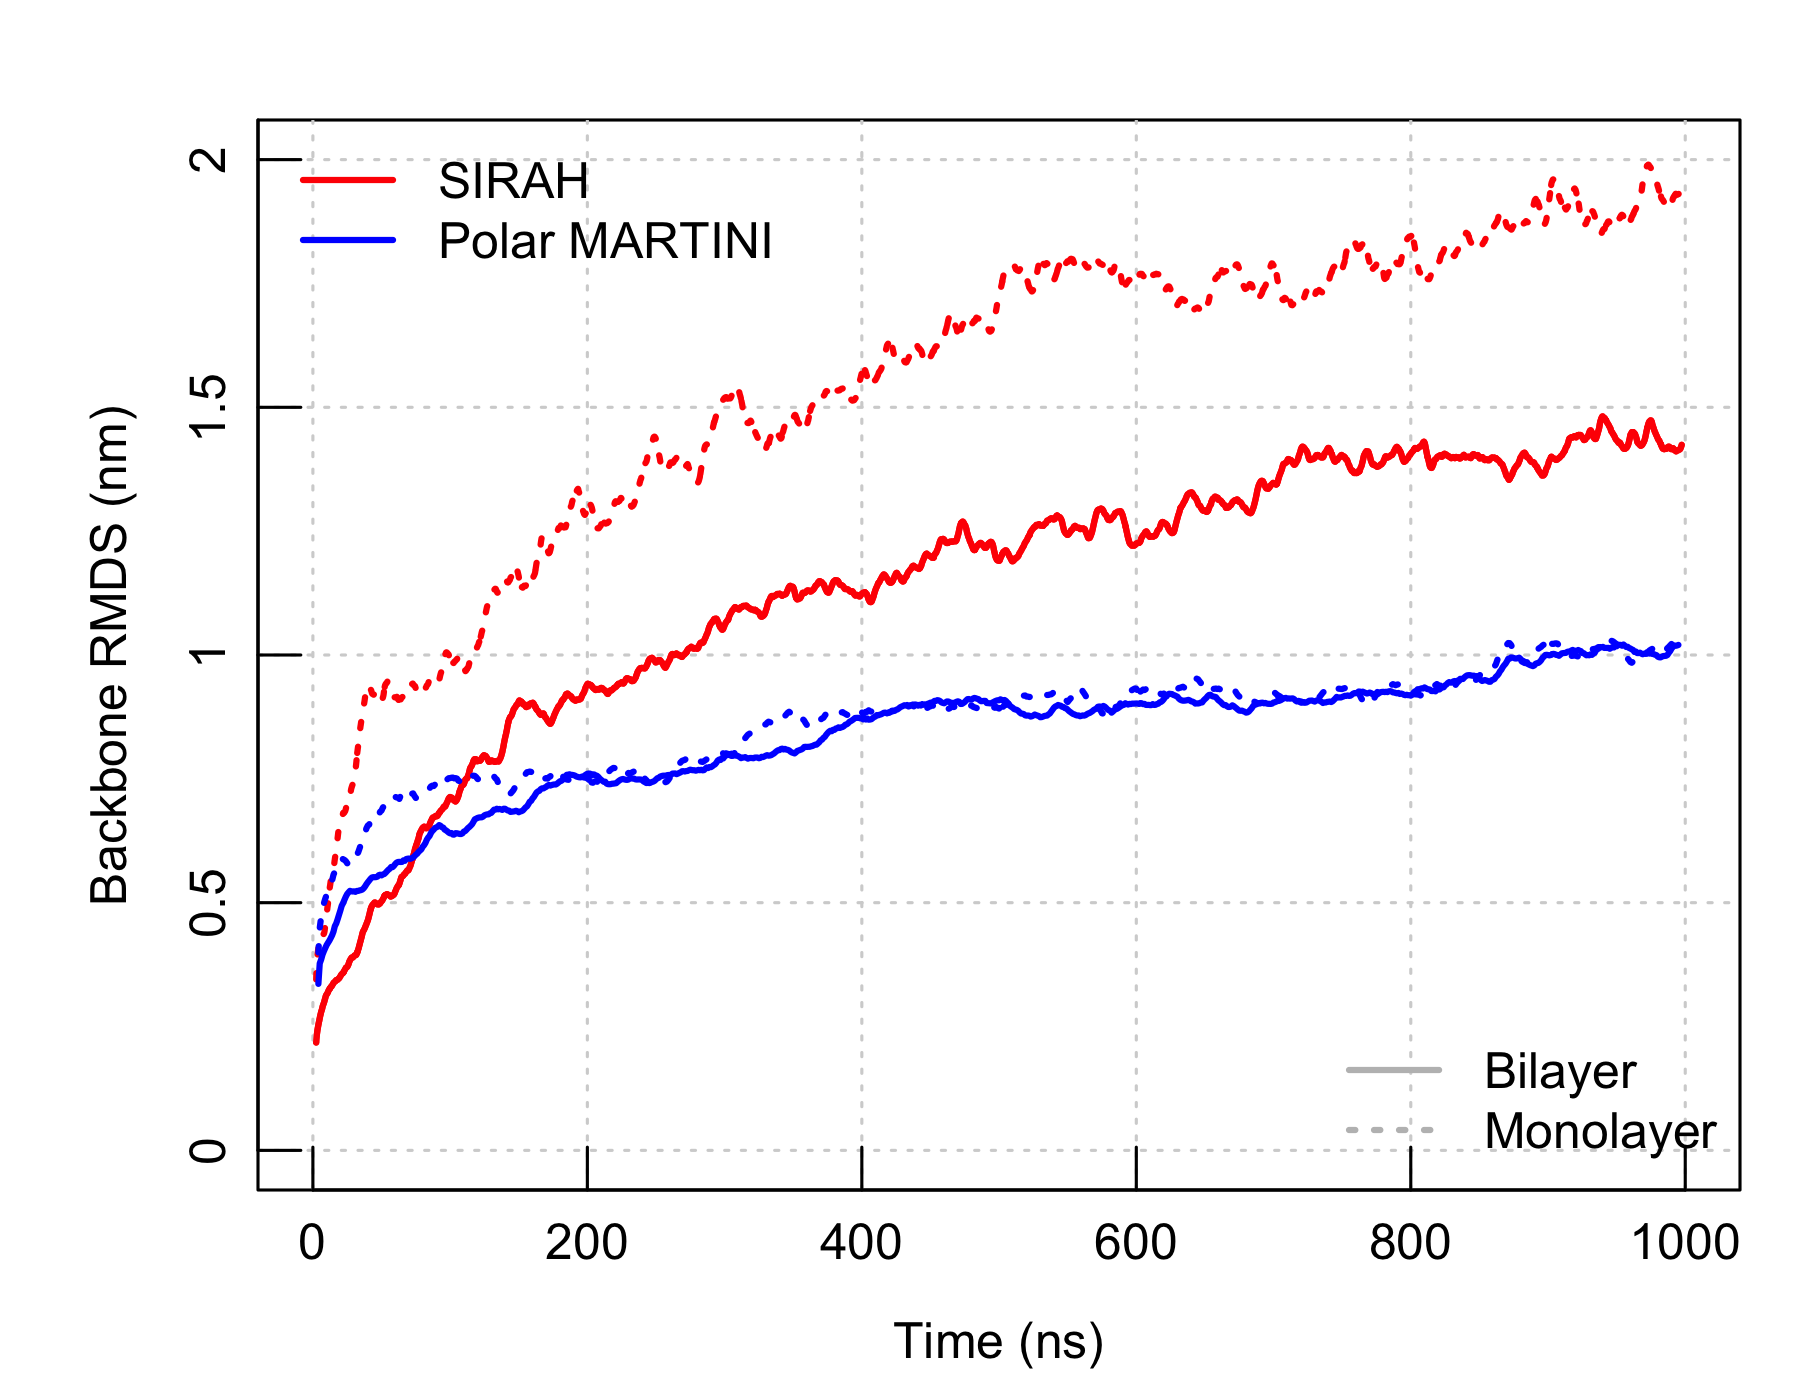
\includegraphics[width=\linewidth]{3results_capsule/pics/compare_MonoBi_rmsd.png} \\
        \subbottom[]{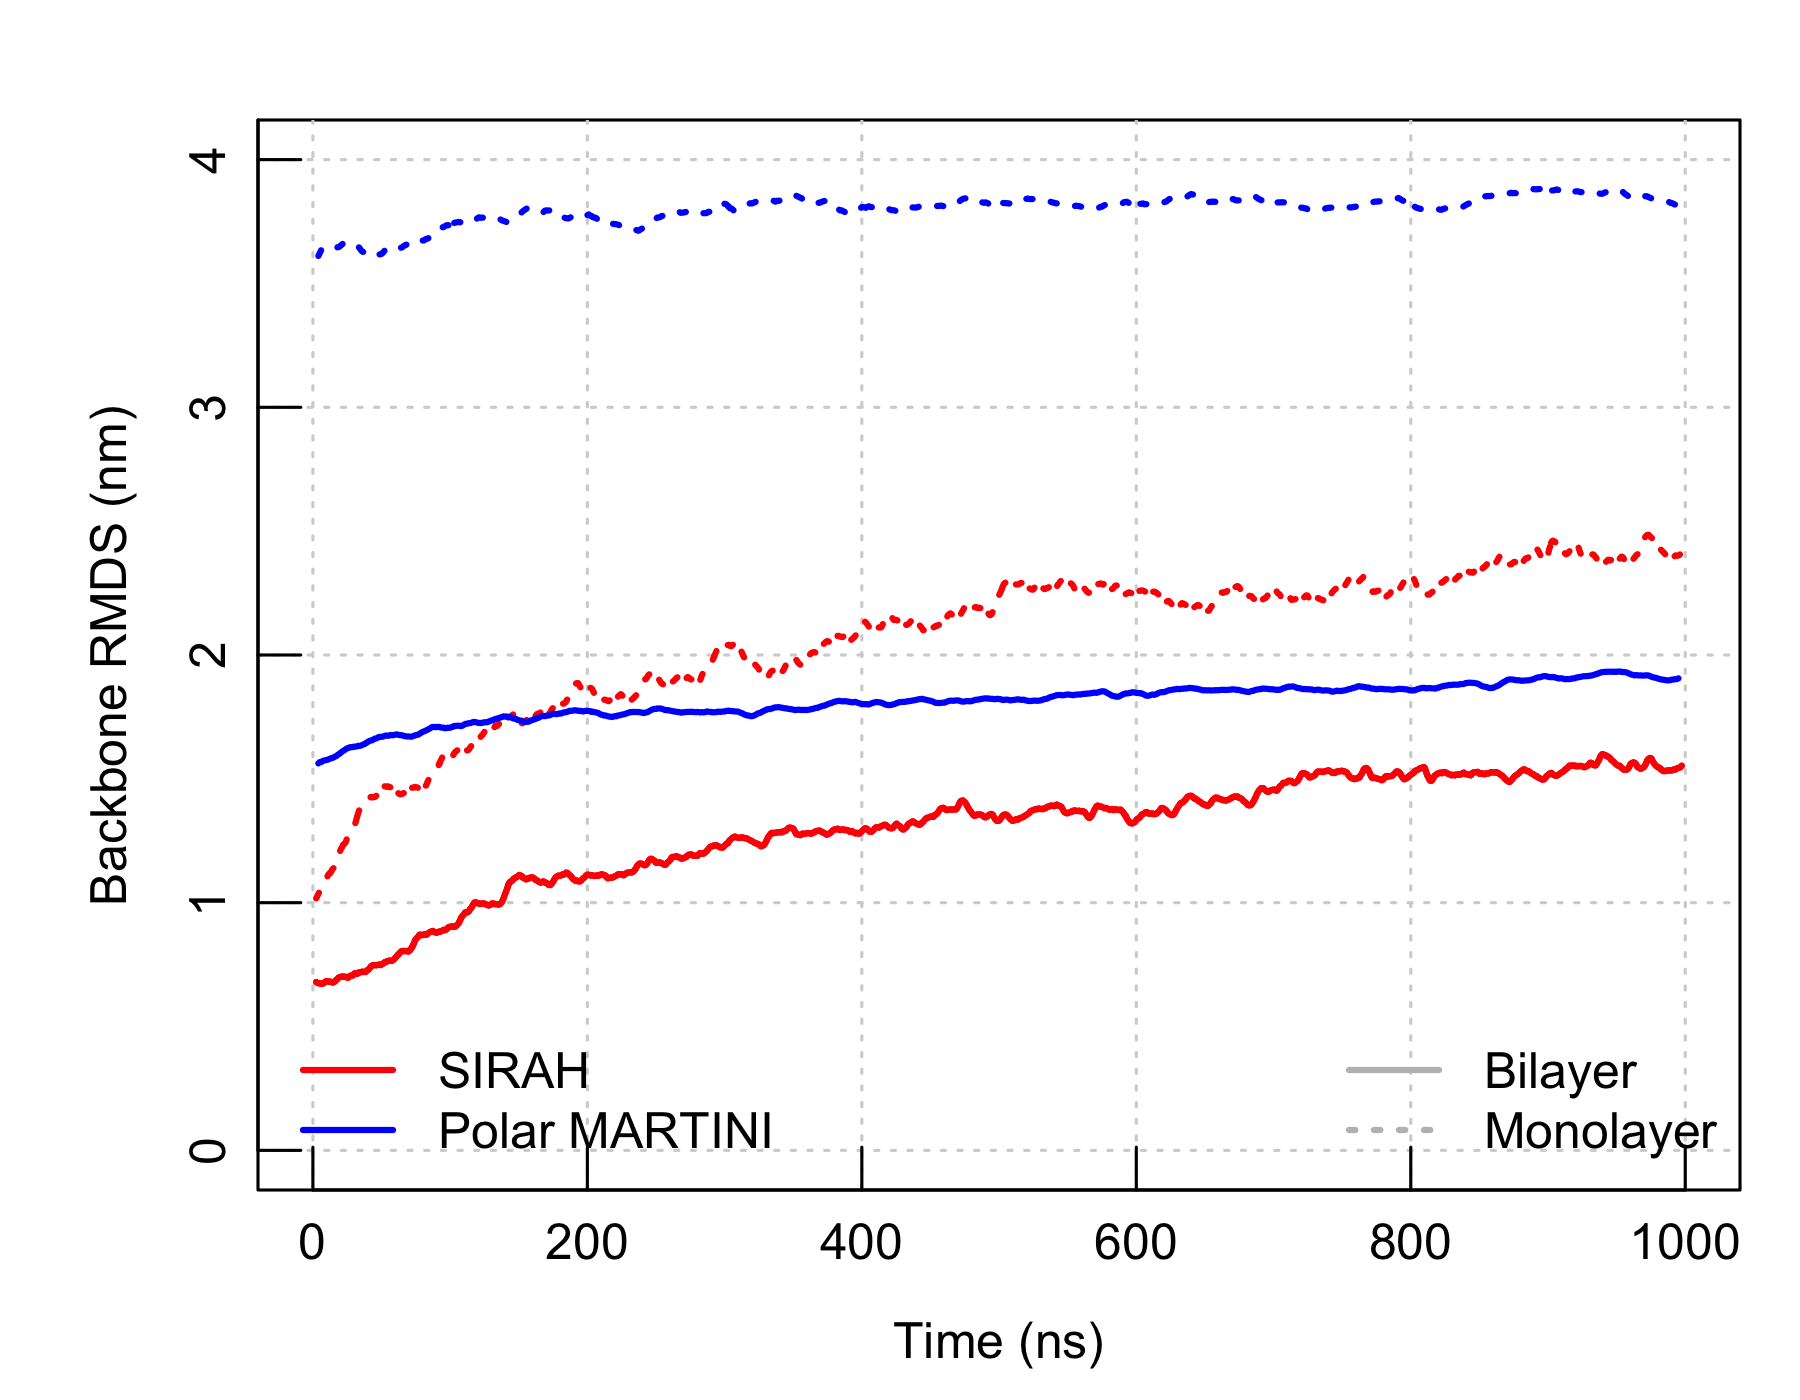
\includegraphics[width=\linewidth]{3results_capsule/pics/compare_MonoBi_rmsd_init.png} \label{fig:rmsd_mono_bi}}
    \end{minipage}
    \begin{minipage}[c]{0.48\textwidth}
        \subbottom[]{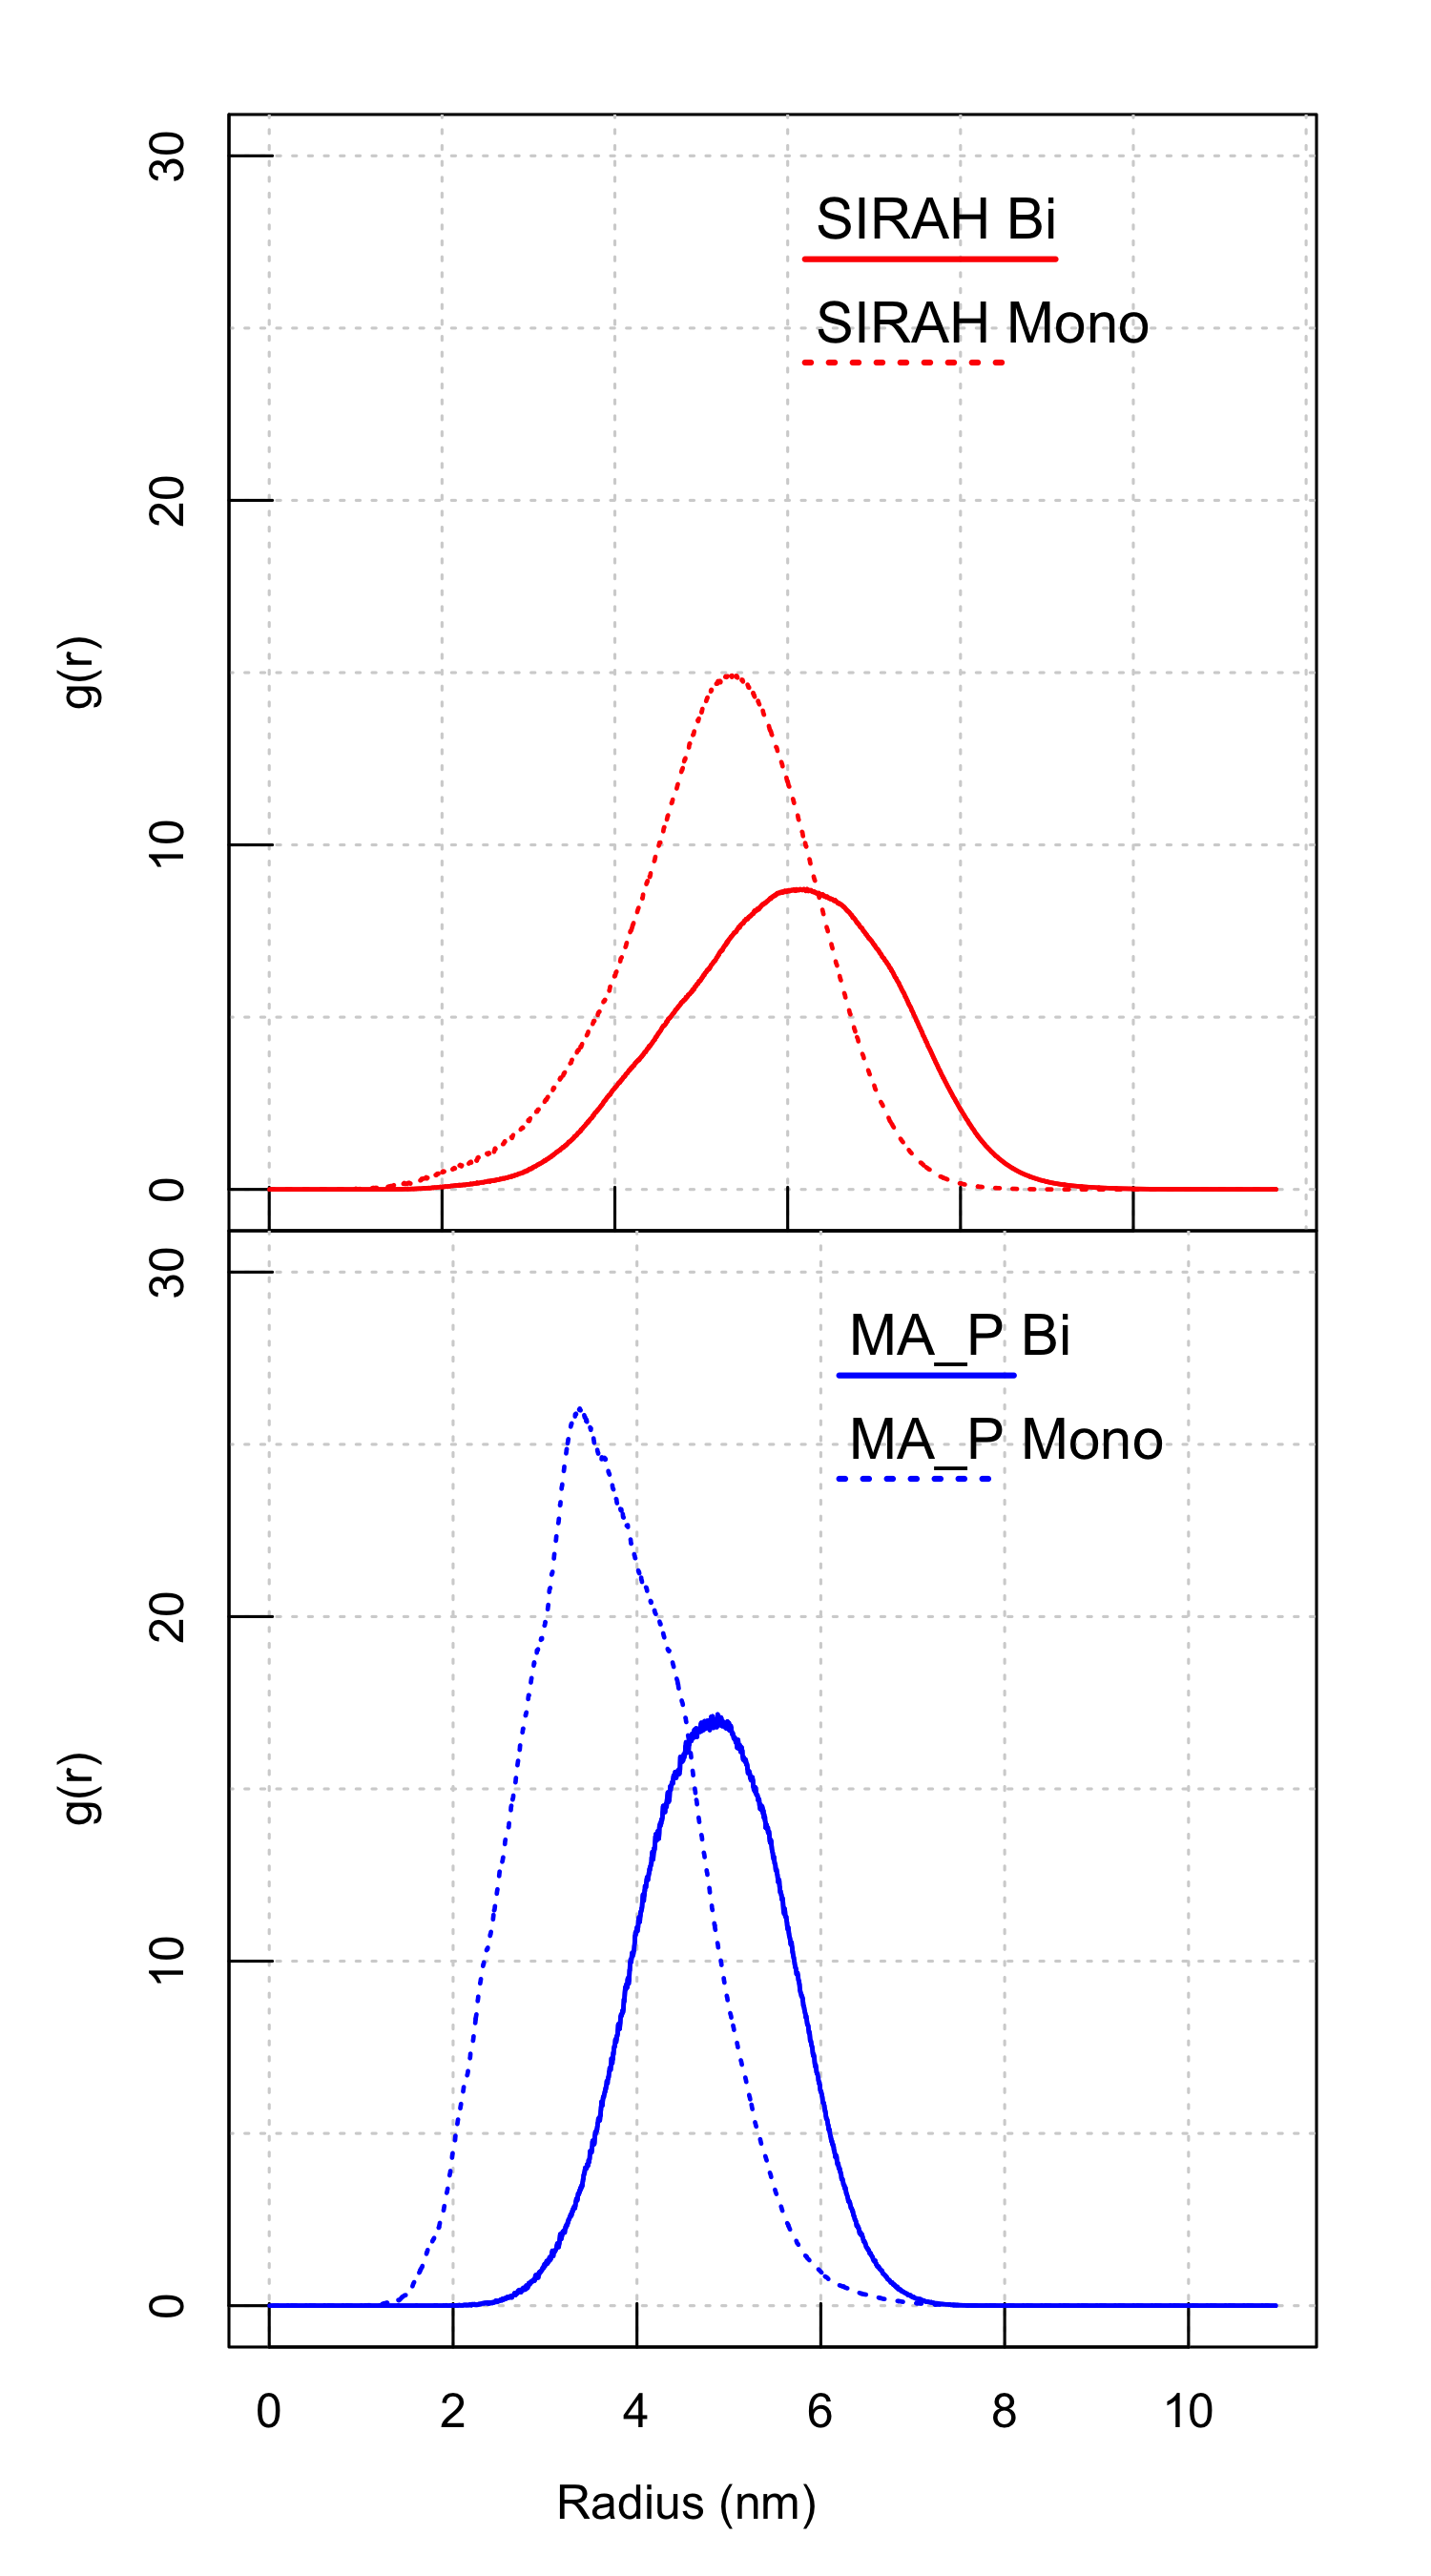
\includegraphics[width=\linewidth]{3results_capsule/pics/compare_MonoBi_RDF.png} \label{fig:rdf_mono_bi}}
    \end{minipage}
    \caption[Comparison of structural properties between monolayer and bilayer structures]{(a) RMSD of the monolayer and bilayer structures along the production run, for the SIRAH and Polar MARTINI force field, with respect to the initial structure of the production (top), and initial geometrical configuration (external layer of Figure \ref{fig:BTI_vmd_3}). (b) RDF of Protein masses around their center of mass. For each label of the legend, the bar has length of the respective RDF FWHM (thickness estimate). \textbf{[DO BARS]} Results are shown for Replica 1 of each simulation setup.}
\label{fig:mono_bi}
\end{figure}


\begin{figure}[h!]
\centering
\subbottom[]{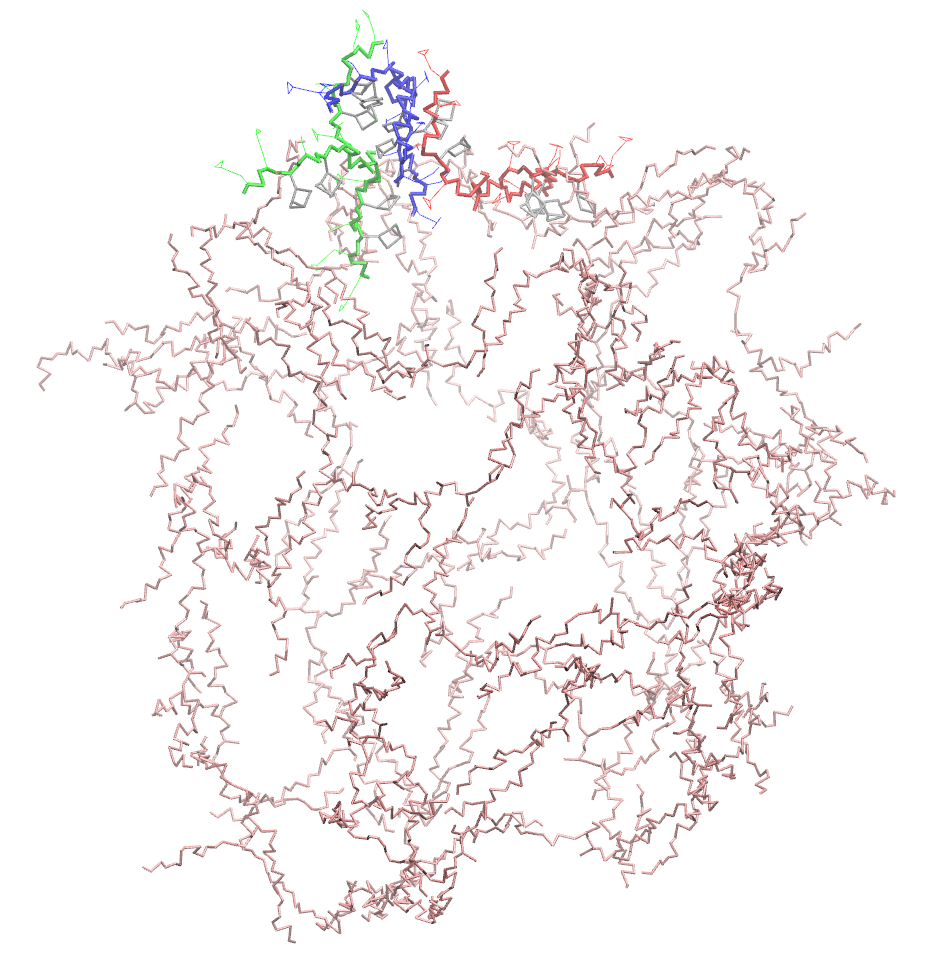
\includegraphics[width=0.48\linewidth]{3results_capsule/pics/sirah_mono_all.png} \label{fig:sirah_mono_all}}
\subbottom[]{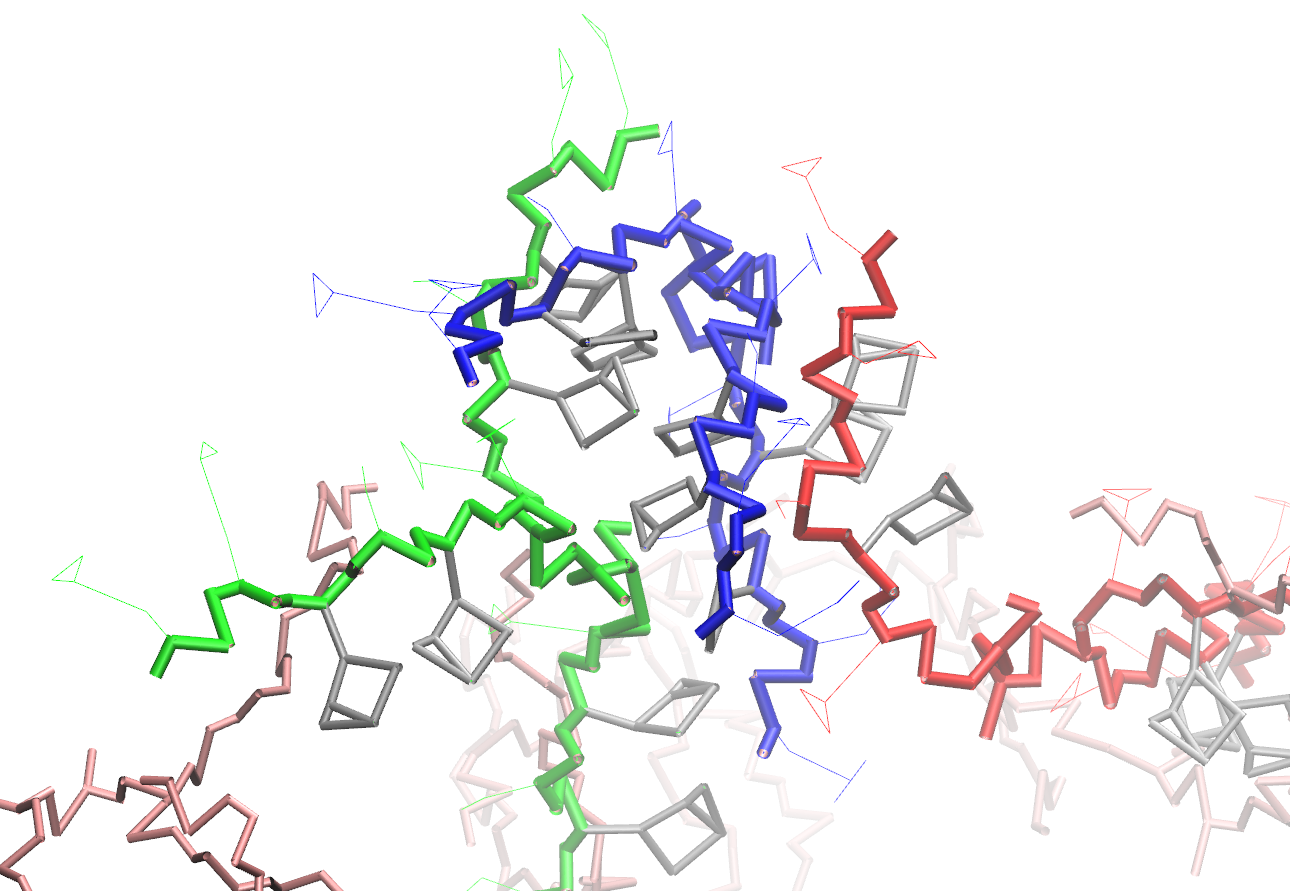
\includegraphics[width=0.48\linewidth]{3results_capsule/pics/sirah_mono_detail.png} \label{fig:sirah_mono_detail}} 
\caption[Snapshot of SIRAH monolayer simulation]{\textbf{[REDO]} (a) Final configuration of a SIRAH monolayer simulations (Replica 1), with highlighted a protruding puckered structure recurrently occurring several positions of the capsule. (b) Detail of the puckered structure. Representations: backbone of the full structure in pink bonds; backbone of highlighted triskelion molecules in green, blue and red bonds; side chains of selected molecules in green, blue and red lines, excluded Tryptophan, in silver bonds.}
\label{fig:sirah_mono_pic}
\end{figure}


\begin{figure}[p!]
\centering
\subbottom[]{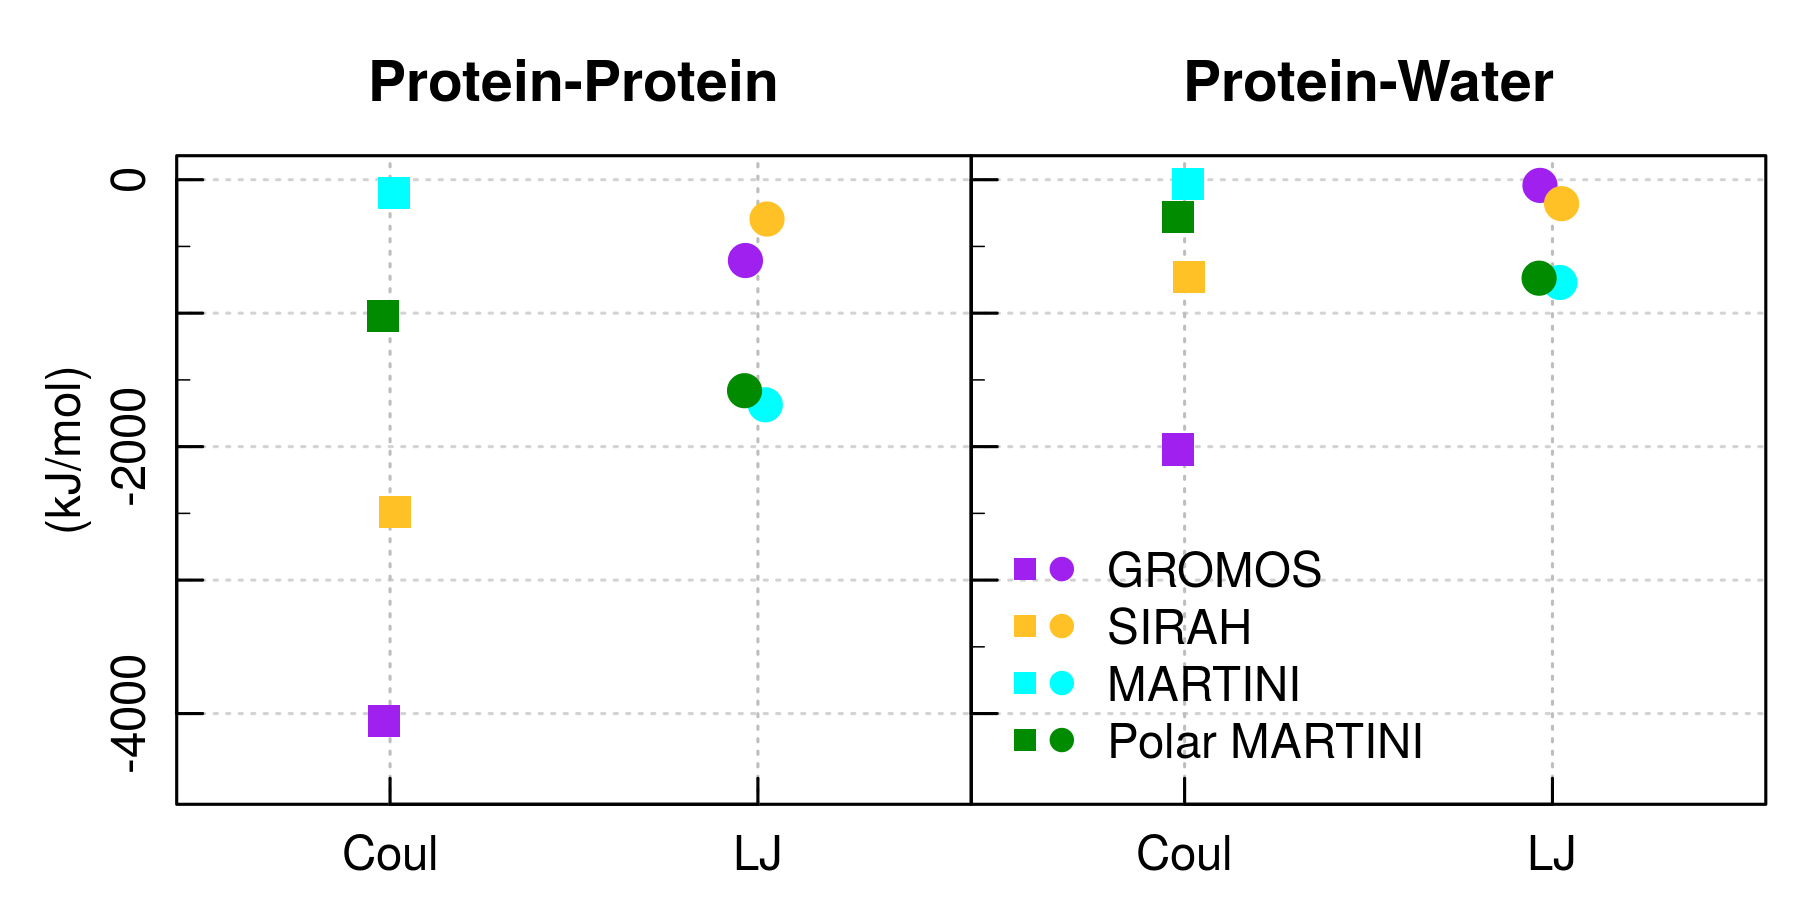
\includegraphics[width=0.8\linewidth]{3results_capsule/pics/many_energies_brief.png} \label{fig:value_eng_cg}} 
\caption[Non-bonded protein energy contribution to capsule structures]{(a) Protein-Protein and Protein-Water non-bonded interactions, normalised per molecule.}
\label{fig:eng_cg}
\end{figure}







\section{Rest}


\clearpage


%\begin{figure}[h]
%\centering
%%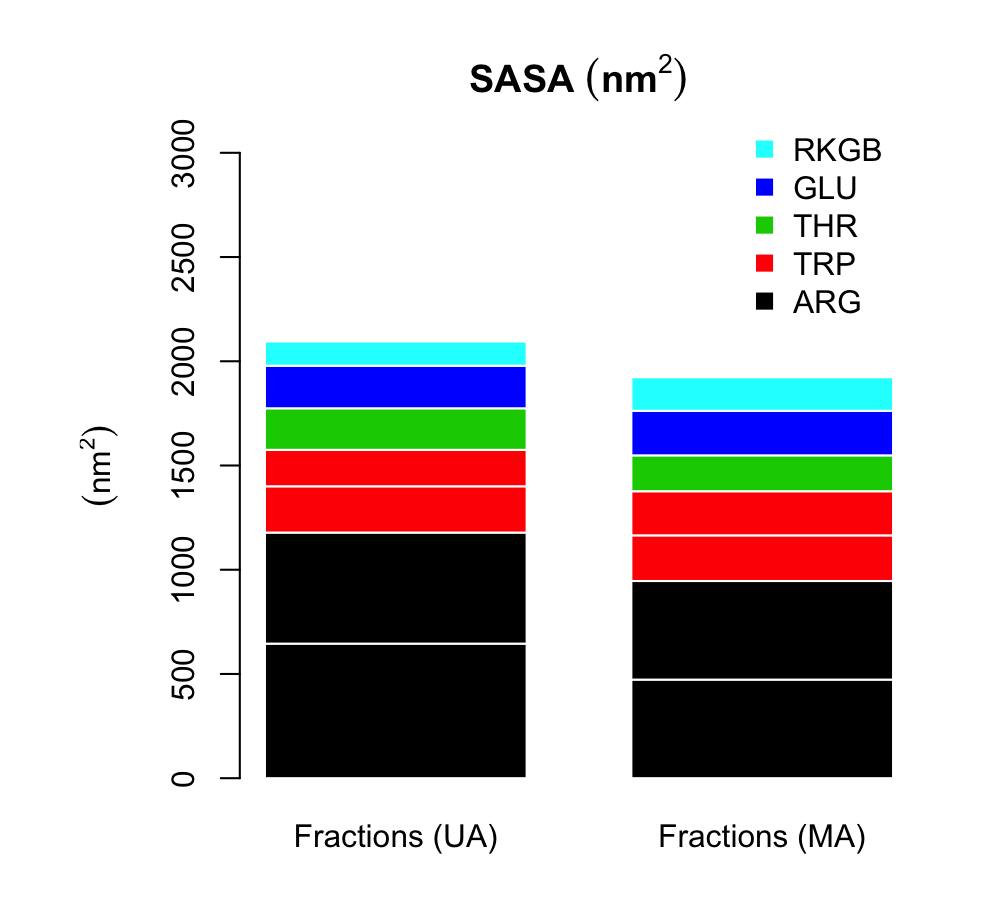
\includegraphics[width=0.5\textwidth]{pics/noSI_stAll_sasa_fractions.png}
%\caption{\textbf{[REDO BETTER AND PUT PANEL LETTER]} Break down of the total Solvent Accessible Surface Area (SASA) in the residue types of which the molecule is composed. }
%\label{fig:BTI_sasa_exposed}
%\end{figure}


%\paragraph{Backmapped simulations} Two of the coarse grain MARTINI final configurations are backmapped to atomistic resolution, and they are simulated for additional 200 ns. The structures expand and their sizes tend to the one obtained in direct atomistic simulations (SI Figure \ref{fig:backmap_Rg_SI} shows the evolution of the radius of gyration).
%%
%The pattern of contacts per residue from backmapping, computed on the last 100 ns of simulations, resemble the one found for the original atomistic simulations, except for the backbone ones, which are still influenced by their initial coarse grain configuration. This suggest that the interaction of the side chains is very strong and thus quickly restored after the backmapping, pointing out the role of charge-charge recognition for the cohesion of the system. 
%
%
%is similar to the one in direct atomistic simulations (SI Fig. \ref{fig:SI_BTI_contacts}, bottom), and some of the amino acid type patterns are recovered, like a larger role of Tryptophan in the interactions and less contacts for Threonine.
%
%
%\subsection{Simulation of the peptide on a membrane}
%
%%\paragraph{Effect of peptide on the membrane and electroporation experiments}
%The effect of multiple copies of the peptide on a model membrane is assessed simulating the pentameric 10 molecules assembly on a 512 lipids patch (of composition DLPC/DLPG, 3:1 ratio) for 500 ns and monitoring the Area per Lipid (ApL) and diffusion coefficient.
%%
%ApL is computed from the area of the simulation box in the xy plane (parallel to the membrane), divided by the member of lipids. This measure is accurate when the membrane does not present major curvature, which is the case for the systems in exam.
%%
%The lipids lateral diffusion coefficient (D) is computed as the slope the mean square displacement of their phosphate atom in function of time (fit restricted to the timescale where the behaviour is linear). For simulations in presence of the peptide this is averaged over the lipids on the peptide-free leaflet.
%
%For a system of 512 lipids size, the ApL in presence of the peptide is reduced by 9\% with respect to the value for the pure membrane simulation, and the diffusion coefficient D has a 6-fold reduction for each specie of lipid (Figure \ref{fig:lipids_ApL}, lines 1 to 4). A quantitatively similar effect is observed applying on the membrane an electric field of intensity 70 mV/nm or 130 mV/nm (Figure \ref{fig:lipids_ApL}, lines 2 and 3).
%%
%There are no experimental values for the ApL of the mixture simulated, however experimental values of D below 1 $\mu m^2$/s fall in the regime of gel-like behaviour [[Ref?]]. This is supported by the fact that ApL and D reach similar values for different fields and for the simulations with peptide: when the gel-like phase is reached, much higher perturbations are necessary to further shrink the membrane.
%
%\begin{figure}[t]
%\centering
%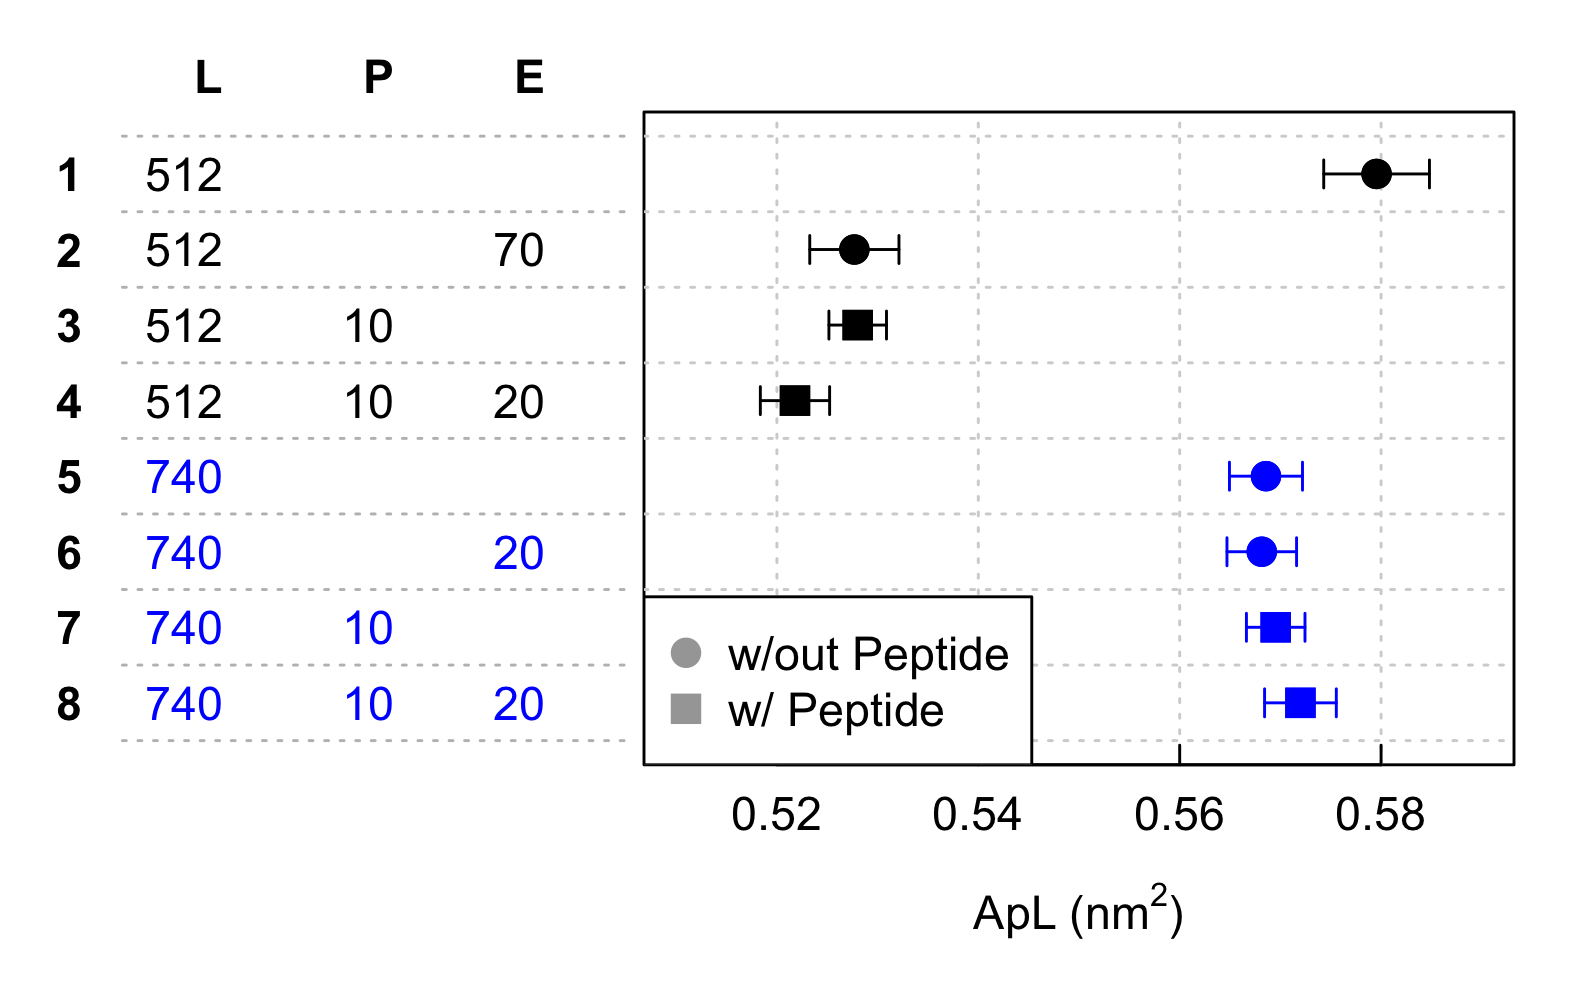
\includegraphics[height=60mm]{pics/apl.png}
%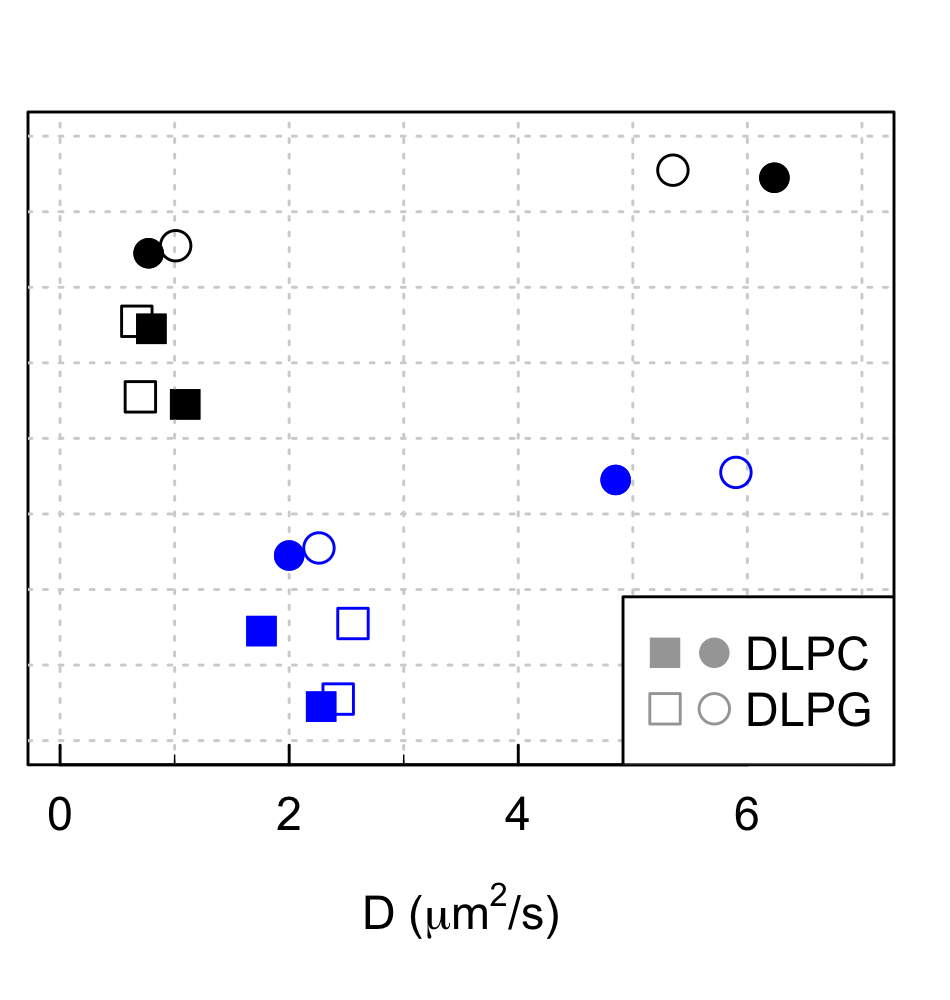
\includegraphics[height=60mm]{pics/diff.png}
%\caption{Area per lipid (ApL, panel a) and lateral lipid diffusion coefficient (D, panel b) from membrane patches simulated under different conditions. On the left a schematic of the system set up is showed (L number of lipids, P number of peptides, E electric field applied in the z direction, in mV/nm ). Black points refer to simulations on 512 lipids patches, blue ones on 740 lipids patches; squares denotes presence of peptide molecules; in panel b full symbol are for DLPC and hollow for DLPG. Bars denote the standard error; for the diffusion coefficient, these are smaller than the point size.}
%\label{fig:lipids_ApL}
%\end{figure}
%
%On the contrary, a different response to external perturbation is observed on a larger patch (Figure \ref{fig:lipids_ApL}, lines 6 to 9): likely larger systems can accommodate better the perturbation and thus no influence in the ApL is observed under the effect of a 70 mV/nm electric field or the peptide, while the diffusion coefficient was still significantly affected.
%
%These findings suggest that the peptide rigidifies a model bacterial membrane due to its high positive charge, which produce an electric field interacting strongly with the anionic lipid species. To investigate whether the peptide has a more specific action on the membrane and which residues are involved in it, we performed electroporation simulations.
%%
%Specifically, to observe the peptide-induced poration mechanism within the simulation time, an electric field of increasing intensity is applied in the negative z direction perpendicular to the membrane, with the peptide on the positive z side, to model the field generated by the transmembrane potential.
%%
%This will allow to accelerate the process, which can be compared with peptide-free electroporation.
%
%\begin{figure}[t]
%\centering
%\begin{minipage}[b]{0.26\linewidth}
%\centering
%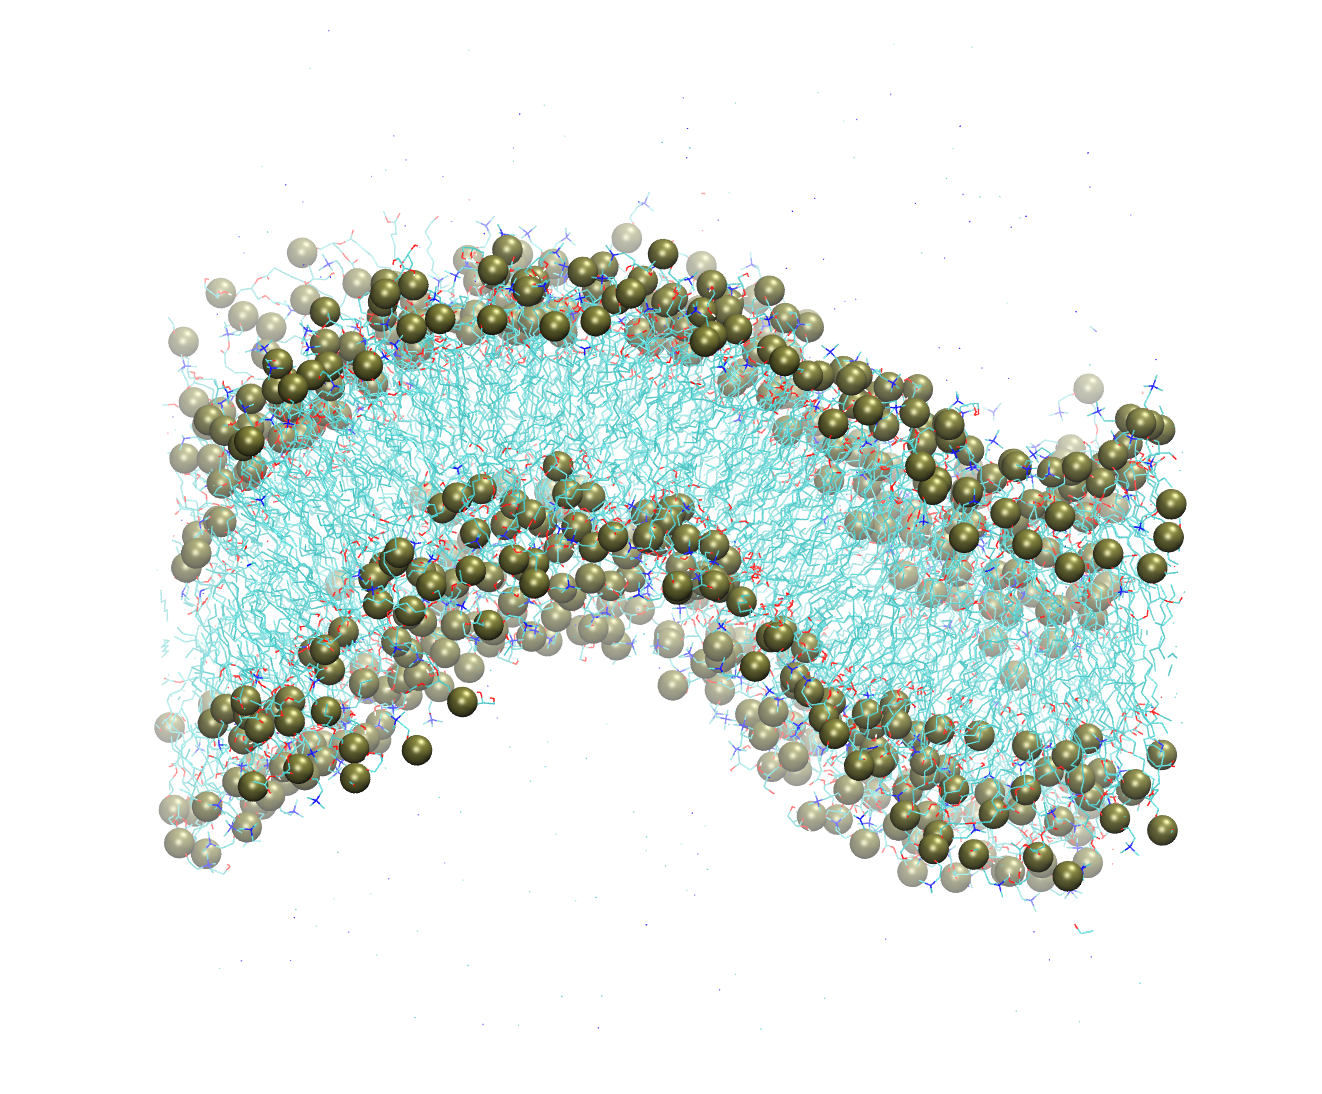
\includegraphics[width=45mm]{pics/cg-130_600ns.png}
%\caption{}\label{fig:pore_pics_1}
%\end{minipage}
%\begin{minipage}[b]{0.4\linewidth}
%\centering
%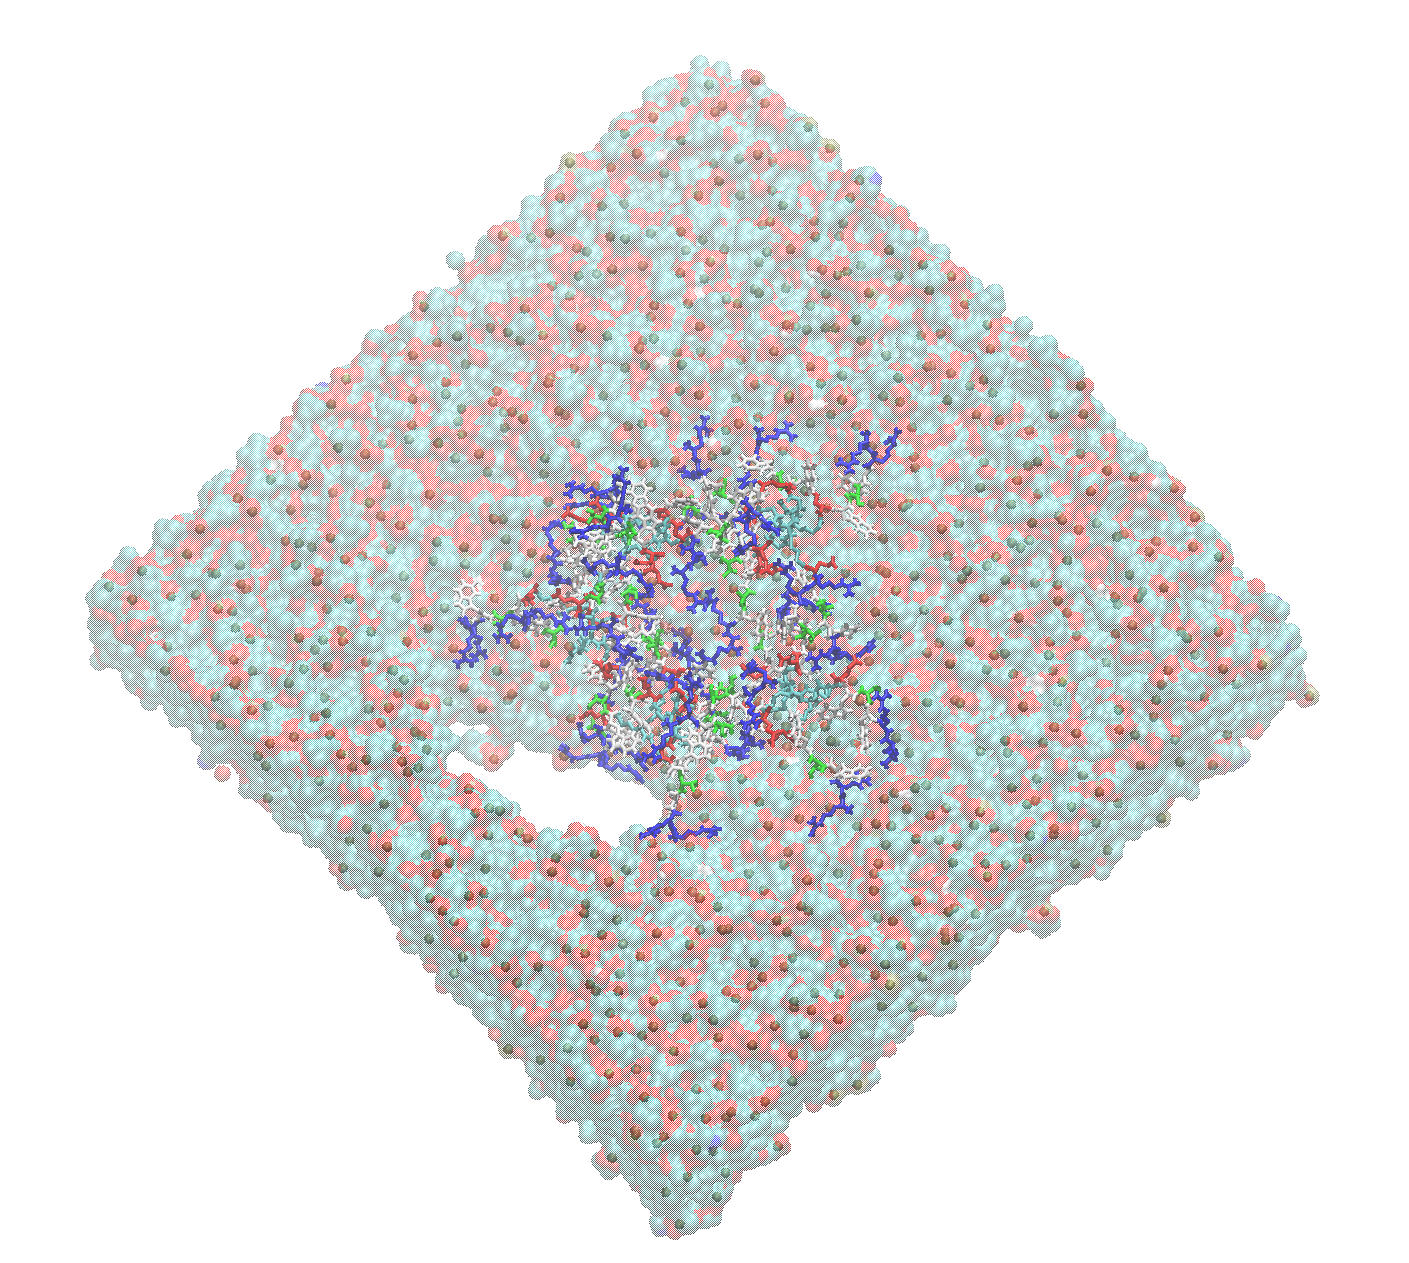
\includegraphics[width=60mm]{pics/pore_large_130.png}
%\caption{}\label{fig:pore_pics_2}
%\end{minipage}
%\begin{minipage}[b]{0.26\linewidth}
%\centering
%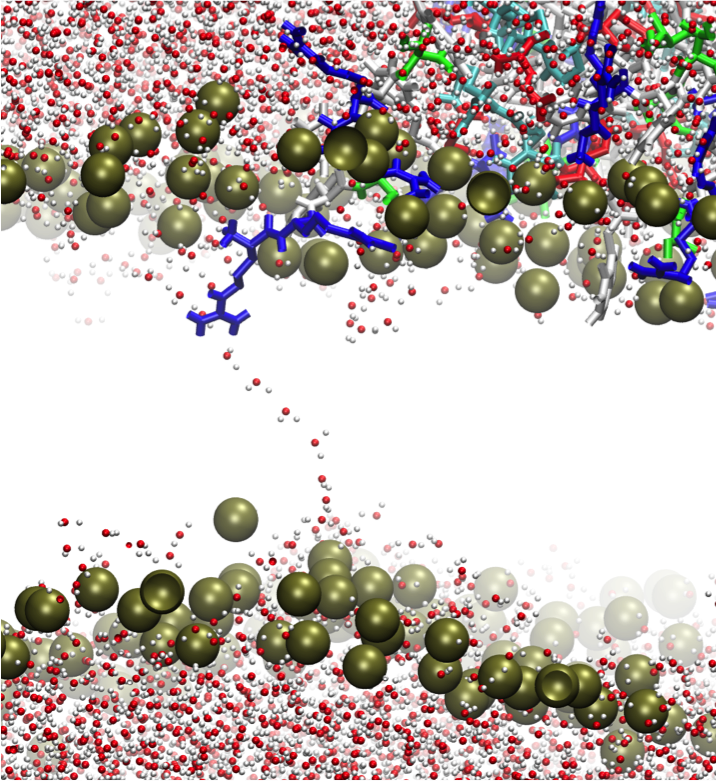
\includegraphics[width=40mm]{pics/pore_arg.png}
%\caption{}\label{fig:pore_pics_3}
%\end{minipage}
%\caption{Panel a: Membrane deformation due to an electric field applied to the membrane (512 lipids, E = -130 mV/nm). Panel b: pore formation due to the action of the peptide. Panel c: pore precursor due to Arginine insertion and water penetration.}
%\label{fig:pore_pics}
%\end{figure}
%
%A test run (on 512 lipids patch), where the absolute magnitude of the field is increased of 20 mV/nm every 200 ns (or 10 mV/nm when approaching the poration threshold), shows that the critical value of 130 mV/nm triggers poration in presence of the peptide. This is confirmed by three replicas run from the initial unperturbed membrane configuration with a 130 mV/nm field, all resulting in poration after 20 ns, 75 ns and 71 ns respectively (Figure \ref{fig:pore_pics_2}).
%%
%Similarly, for simulations with the same field on a larger patch (740 lipids) poration occurs at 60 ns, 50 ns and 70 ns respectively.
%%
%As a control, a membrane alone  (512 lipids patch) is simulated for 600 ns in three replicates with the same field: despite a reduced area per lipid and diffusion coefficient, no poration was observed. The electroporation threshold for the membrane alone is set at the higher value of 140 mV/nm: out of three simulations run with such value of the electric field, one resulted in disruption at 160 ns, while the other two presented a curved but still intact membrane after 200 ns (Figure \ref{fig:pore_pics_1}).
%
%These simulations also shows that the poration mechanism is different when caused by an electric field or by the peptide (in cooperation with a field).
%%
%In the electroporation case, the disruption is preceded by curvature of the membrane which in turn is caused by local deviations of the z-position of single lipids with respect to the membrane plane. As these bear local charge imbalance, they are enhanced by the electric field and when one of the leaflet is stretched water molecules are allowed to penetrate inside the hydrophobic core of the membrane and grow into a pore.
%
%When the peptide is present instead, the charged Arginine residues insert into the membrane core interacting with the negatively charged phosphate of the lipids, and promote the penetration of water molecule (Figure \ref{fig:pore_pics_3}).
%%
%In already curved regions, this causes pore formation even if the curvature is not sufficient for electroporation itself.
%%
%Additionally, the peptide enhances the invagination of the membrane and these two aspects together (stronger invagination and Arginine insertion) allow pore formation at a value of the electric field lower than the one necessary for electroporation.
%
%
%%\paragraph{Local perturbation to membrane structure}
%To understand the local effect of the peptide, we compute the diffusion coefficient for lipids based on their distance from the peptide: the ones whose phosphorus atom is within 1 nm from the protein, within 2 nm, 3 nm and finally the ones more distant than 3 nm, which include the majority of the bottom leaflet (Fig. \ref{fig:msd_increase}).
%%
%The value of D increases including more distant lipids, but they all diffuse less than in an unperturbed membrane (this is valid also for the ones in the leaflet opposite to the peptide).
%%
%Lipids nearby the peptide are partially restrained to the position of the latter though a network of electrostatic and hydrogen bond interactions. The majority of hydrogen bonds formed involve Arginines (long life bonds) and Tryptophans (short life ones).
%%
%In the simulation of a large patch and the ten molecules peptide, 62 hydrogen bonds are present for more than 40\% of the time, and more than half of them involve Arginines (38, of which 25 with DLPC molecules, and 13 with DLPG ones). Tryptophan residues instead interact through short life bonds (140 of them are present at each time point on average, but only 11 for more than 40\% of the time).
%%
%The fact that the peptide influence is long range and extends to lipids not directly in contact with itself is likely due to the ``viscous" character of the membrane: around the restrained lipids, the other molecules move slower and the unperturbed diffusion ratio is reached only at larger distances.
%
%This findings, together with the previous results, suggests that the rigidification process (measured by the reduction of the diffusion coefficient), regardless the membrane compactness (measured by the area per lipid), is a proxy for poration as it makes the lipids less able to accommodate perturbations and to seal a forming water channel.
%
%\begin{figure}[t]
%\centering
%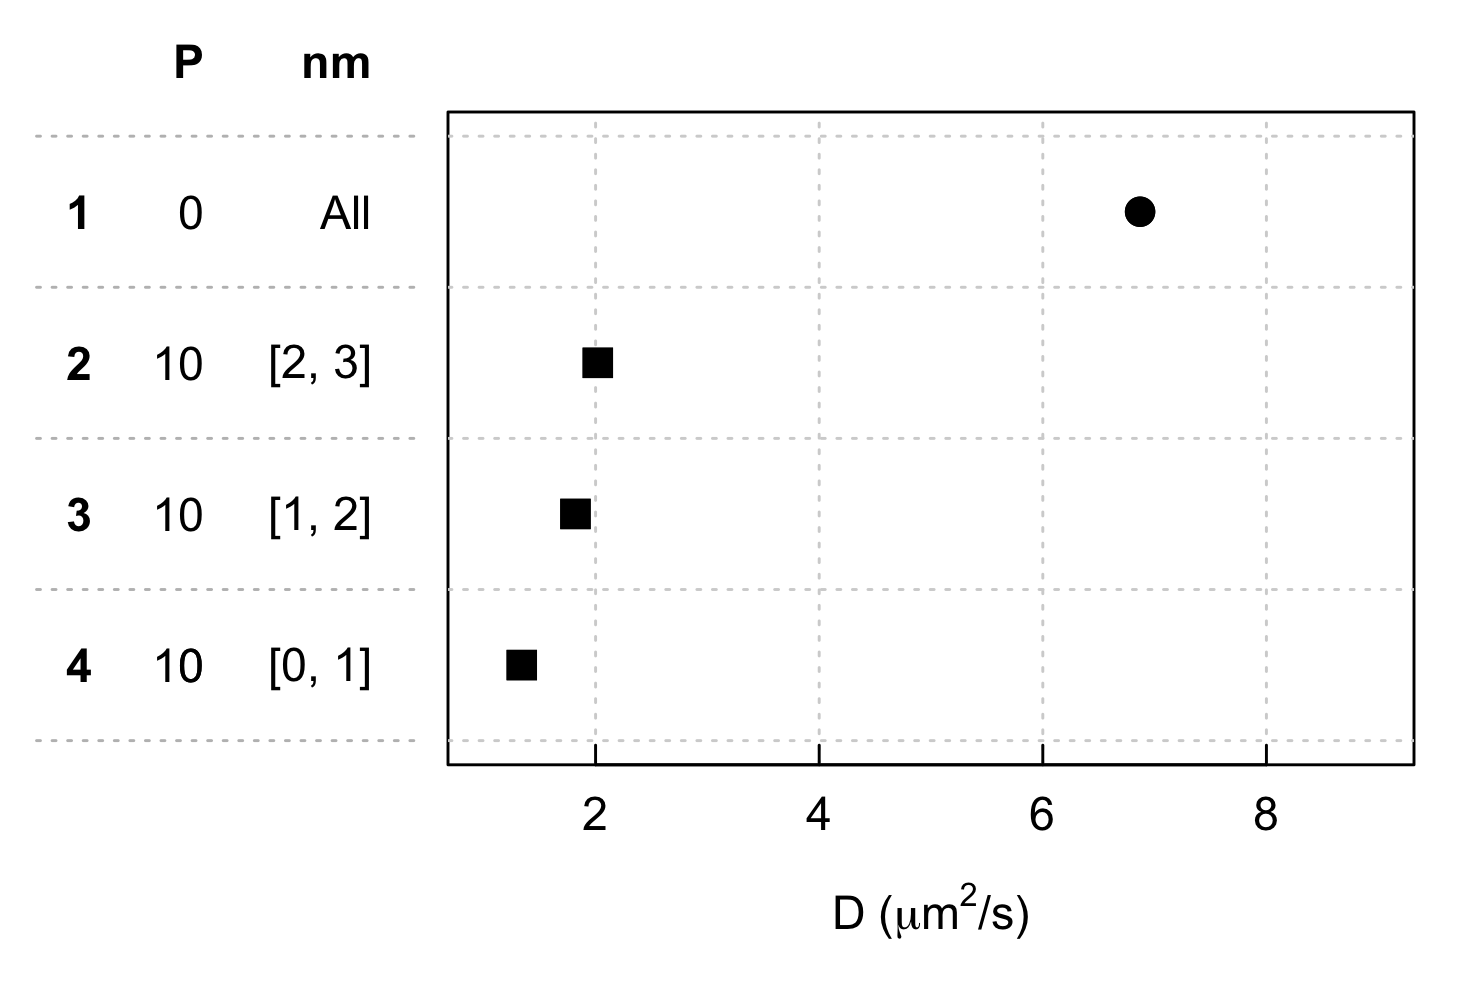
\includegraphics[width=0.7\textwidth]{pics/D_distance.png}
%\caption{Diffusion coefficient of the lipids within given distance from the protein. P: number of peptide on the membrane, nm: interval of distances between the peptide and the lipids selected for the computation. }
%\label{fig:msd_increase}
%\end{figure}
%
%%\paragraph{Membrane binding mechanism}
%A coarse grain simulation of the full buckyball on a DLPC:DLPG membrane (3:1 ratio) confirms the binding of the peptide on the latter, driven from charge-charge recognition: in both the replicas run, the peptide approaches the membrane after about 2 $\mu$s, remaining bound up to the 10 $\mu$s simulated (the binding happens on opposite leaflets of the membrane, proving that it is not biased by the initial configuration).
%%
%Post-binding, the capsule diffuses on the membrane and produces an increasingly high curvature on it, in a process which tends to maximize the contact area (see SI Movie --). No poration is observed, probably due to the force field characteristics which stabilise the structure of both the membrane and the peptide assembly or the short time scale simulated.
%%
%The lipids diffusion coefficient is decreased after the binding, by 9\% for DLPC and by 15\% for DLPG (see SI Table \ref{table:SI_martini_diff} and SI Figure \ref{fig:SI_martini_lipids_bound}).
%Moreover, as DLPG is negatively charged, it is recruited around the peptide and remain bound to it, diffusing much slower than the surrounding lipids.
%
%A control simulations with a pure DLPC membrane shows no binding of the peptide: the distance of the icosahedron from the membrane is on average 3 nm and never smaller than 1 nm. This does not exclude a binding on longer time scales, but hints at the fact that, not being driven by the opposite charge recognition, the peptide-membrane interaction is weaker and less likely to happen.
%
%
%\section{Conclusions}
%
%In the present work, we propose a model structure for the three dimensional arrangement of a novel antimicrobial peptide, testing the stability of the proposed model by means of Molecular Dynamic simulations. Furthermore, we investigated the details of its antimicrobial activity simulating its interaction with a model bacterial membrane.
%
%The simulations performed on the peptide assembly and on its subunits highlighted the preferred conformations: a staggered $\beta$-sheet favouring Tryptophan interactions and the stacking of $\beta$-sheets pairs to confer stability to the assembly by screening the hydrophobic residues and to grant rigidity.
%%
%The structure of the single molecule suggests an ordered geometry of the supra molecular assembly to optimise the number of interaction between peptides, however the simulations proved that the molecule is not rigid enough to form a virus-like cage, while a dynamical equilibrium is enforced in which the components have the freedom to fluctuate around the equilibrium position.
%
%These findings are important to direct future design of similar molecules, as the rigidity and mechanics of the capsule structure are crucial to tune its function as carrier and its interactions with the host cells.
%
%Regarding the interaction with a bacterial cell instead, simulations make clear that the peptide has a complex effect on the membrane, prior to its disruption: its presence enhance its rigidity, making it prone to disruption upon local triggers such as Arginine insertion. This support the necessity of a self-assembling antimicrobial peptide, as the higher the local concentration of antimicrobial molecules, the more the deviation from the base line membrane properties, which favours an early disruption.
%
%Overall, the work shows how Molecular Dynamics simulations give precious information on the atomistic-level mechanisms underlying mesoscopic processes: despite the limitations of the technique prevent sometimes a quantitative interpretation of the simulations result, MD proves the qualitative aspect of various processes and can be effectively used to compare different systems and identify the local characteristics which lead to diversified behaviours. This will suggest the design of new experiment to specifically tackle aspects based on emerged via simulations and thus finally prove the MD findings.
% 

%
%\clearpage
%\section{SI miscellaneous}
%
%\begin{figure}[h!]
%\centering
%\includegraphics[width=0.3\textwidth]{pics/capzip_formula.jpg}
%\caption{From \cite{Castelletto2016}. Chemical structure of the antimicrobial molecule capzip.}
%\label{fig:SI_capzip_formula}
%\end{figure}
%
%
%\begin{figure}[h!]
%\centering
%\includegraphics[width=0.6\textwidth]{pics/hb_beta_poster.png}
%\caption{Presence of hydrogen bonds between backbones of two facing RRWTWE facing chains forming an antiparallel $\beta$-sheets. Residue identified by type and number (1-6 first chain, 7-13 second one). Occupancy average over 16 simulations of 100 ns.}
%\label{fig:hb_beta_SI}
%\end{figure}
%
%
%\begin{figure}[h!]
%\centering
%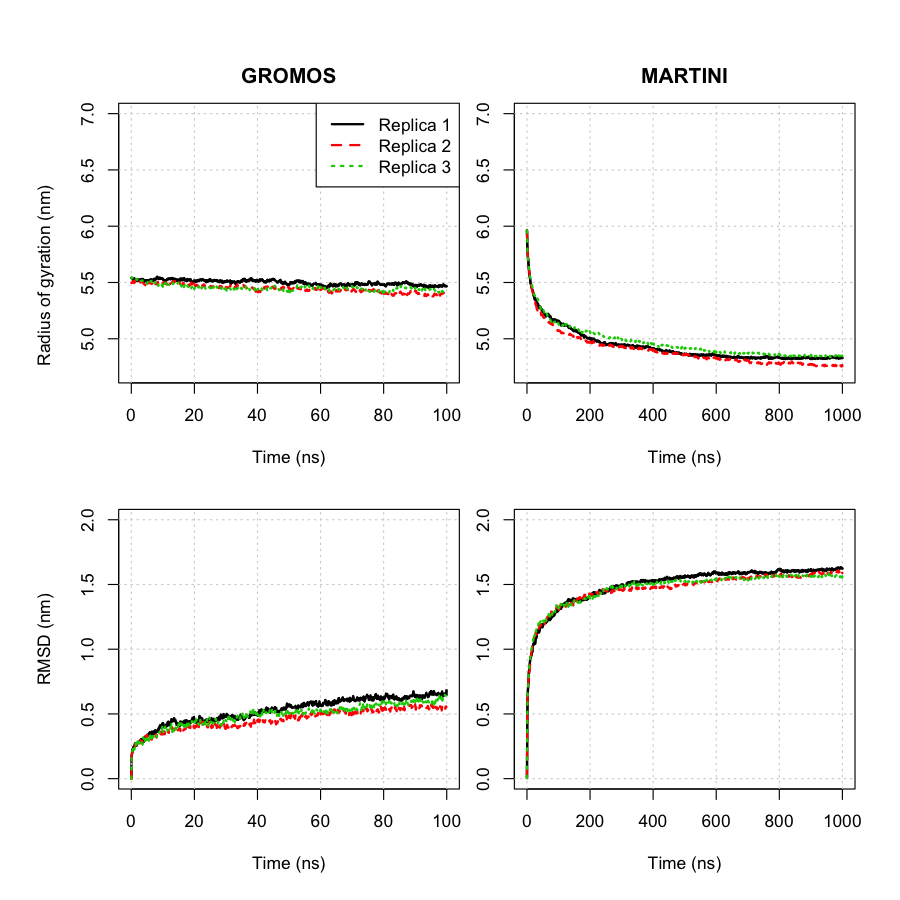
\includegraphics[width=0.8\textwidth]{pics/noSI_stAll_Rg_rmds.png}
%\caption{Radius of gyration and Root Mean Square Deviation (RMSD) for the buckyball in atomistic (GROMOS) and coarse grain (MARTINI) simulations, three replicas each.}
%\label{fig:rg_rmsd_SI}
%\end{figure}
%
%
%\begin{figure}[h!]
%\centering
%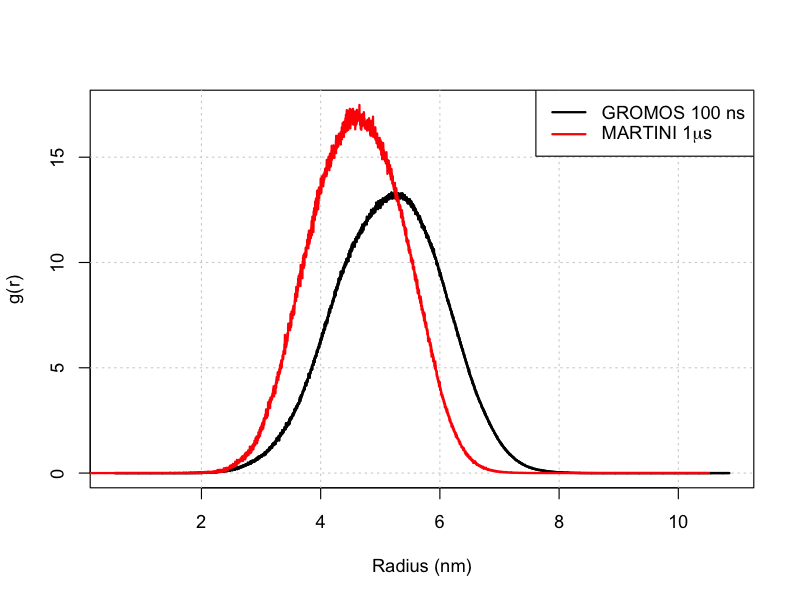
\includegraphics[width=0.6\textwidth]{pics/noSI_stAll_RDF.png}
%\caption{Radial distribution function of Protein masses around their center of mass.}
%\label{fig:rdf_SI}
%\end{figure}
%
%
%\begin{figure}[h]
%\centering
%\includegraphics[width=0.7\textwidth]{pics/HbMix_histo_by_restype.png}
%\caption{\textbf{[REDO BETTER]} Average number of hydrogen bonds between side chains and backbone per molecule occurring in 100 ns atomistic simulations of the buckyball structure.}
%\label{fig:BTI_hbonds_SI}
%\end{figure}
%
%
%\begin{figure}[h!]
%\centering
%\includegraphics[width=0.6\textwidth]{pics/stUA_BM.png}
%\caption{Radial distribution function of Protein masses around their center of mass.}
%\label{fig:backmap_Rg_SI}
%\end{figure}
%
%
%\begin{figure}[h]
%\centering
%\includegraphics[width=0.85\textwidth]{pics/rep1_sch_BM.png}
%\caption{\textbf{[BETTER QUALITY]} Contacts with persistence greater than 50\% during a backmapped atomistic, between C$_\alpha$s (left column), between side chains (middle column) and mixed C$_\alpha$-side chain (right column).}
%\label{fig:SI_BTI_contacts}
%\end{figure}
%
%
%\begin{figure}[h]
%\centering
%\includegraphics[width=0.85\textwidth]{pics/nr_lipids_bound_2nm.png}
%\caption{\textbf{[BETTER QUALITY]} Number of lipids within 2 nm distance from the buckyball in the coarse grain simulation of the buckyball on a model bacterial membrane (two lipid species, DLPC and DLPG, and two replicas run).}
%\label{fig:SI_martini_lipids_bound}
%\end{figure}
%
%
%
%
%\clearpage
%
%\paragraph{Correlation}
%Correlation is computed as the sum of the covariances in the three directions, normalised by the square root of the product of the variance (sum of the variances in the three directions) of the motion of the two atoms. Assuming the $x$-covariance between atom $i$ and $j$ is and the $x$-variance of atom $i$ are:
%\begin{eqnarray}
%\sigma(x_i, \, x_j) &=& \overline{x_i(t) \, x_j(t)} - \overline{x_i(t)} \overline{x_j(t)} \\
%\sigma(x_i) &=& \overline{x_i^2(t)} - \left( \overline{x_i(t)}\right)^2
%\end{eqnarray}
%where the $\overline{\cdot}$ denotes the time average of quantity $\cdot$; then the correlation between the motion of two molecules was estimated as:
%\begin{equation} \label{eq:corr}
%C(i,j) = \frac{\sigma(x_i, \, x_j) + \sigma(y_i, \, y_j) + \sigma(z_i, \, z_j)} {\sqrt{ \left( \sigma(x_i) + \sigma(y_i) + \sigma(z_i) \right) \left( \sigma(x_j) + \sigma(y_j) + \sigma(z_j) \right) }}
%\end{equation}
%
%\vspace{2cm}
%
%
%\begin{figure}[h]
%\centering
% \def\arraystretch{1.5}
%\begin{tabular}{l|r|rr|cc}
% \textbf{System} & \textbf{Nr lipids} & \textbf{E} (mV/nm) & \textbf{[NaCl]} (mM) & \textbf{Time (ns)} & \textbf{Replicas} \\
% \hline
% DLPC:DLPG 3:1 & 512 & 0 & 0 & 400 & 1 \\
% & 512 & 0 & 150 & 400 & 1 \\
% & 512 & -2 & 150 & 200 & 1 \\
% & 512 & -4 & 150 & 200 & 1 \\
% & 512 & -6 & 150 & 200 & 1 \\
% & 512 & -8 & 150 & 200 & 1 \\
% & 512 & -10 & 150 & 200 & 1 \\
% & 512 & -12 & 150 & 200 & 1 \\
% & 512 & -7 & 150 & 400 & 1 \\
% & 512 & -13 & 150 & 600, 600, 500 & 3 \\
% & 512 & -14 & 150 & 200, 200  & 3 \\
% &&&& 160 (Poration) & \\
% &&&&& \\
% &&&&& \\
% DLPC:DLPG 3:1 & 740  & 0 & 0 & 400 & 1 \\
% & 740  & -70 & 0 & 400 & 1 \\
% &&&&& \\
% DLPC & 128 & 0 & 0 & 200 & 1 \\
% & 128 & 0 & 150 & 200 & 1 \\
% &&&&& \\
% DLPG & 128 & 0 & 0 & 400 & 1 \\
% & 128 &  0 & 150 & 200 & 1 \\
%\end{tabular}
%\captionof{table}{Control simulations of lipid membranes (all united atoms representation).}
%\label{table:SI_sim_E}
%\end{figure}
%
%
%\begin{figure}[h]
%\centering
% \def\arraystretch{1.5}
%\begin{tabular}{l|rr}
% \multicolumn{3}{l}{\textbf{MARTINI simulations - capsule on bacterial membrane}} \\
% \hline
% & \textbf{DLPC} & \textbf{DLPG} \\
% \hline
% D pre-binding ($\mu \text{m}^2$/s) & 298.81(3) & 294.14(7) \\
% D post-binding ($\mu \text{m}^2$/s) & 273.11(3) & 249.57(6) \\
% N$_{<\,2\,nm} \ ^a$ & 167(12) & 131(7) \\
% N$_{bound} \ ^b$& 197 & 115 \\
%\end{tabular}
%\captionof{table}{Analysis of lipid diffusion in a coarse grain simulation of the buckyball binding to a model bacterial membrane (DLPC:DLPG 3:1). Data for Replica 1, binding time 2.14 $\mu$s. Protein lateral diffusion after binding to the membrane 16.50(2) $\mu$m$^2$/s. $^a \, $Number of lipids within 2 nm distance from the buckyball in the last 5 $\mu$s of simulations. $^b \, $In a simplistic model in which the dumping of lipid lateral diffusion coefficient is due to some lipids bound to the buckyball, and thus they diffuse at its pace, while the other are free to move as before, it is valid the following equation: $D_{post} = D_{pre} \cdot (N_{lipid} - N_{bound}) + D_{protein} \cdot N_{bound}$.}
%\label{table:SI_martini_diff}
%\end{figure}

